\documentclass{book}
\usepackage[a4paper,top=2.5cm,bottom=2.5cm,left=2.5cm,right=2.5cm]{geometry}
\usepackage{makeidx}
\usepackage{natbib}
\usepackage{graphicx}
\usepackage{multicol}
\usepackage{float}
\usepackage{listings}
\usepackage{color}
\usepackage{ifthen}
\usepackage[table]{xcolor}
\usepackage{textcomp}
\usepackage{alltt}
\usepackage{ifpdf}
\ifpdf
\usepackage[pdftex,
            pagebackref=true,
            colorlinks=true,
            linkcolor=blue,
            unicode
           ]{hyperref}
\else
\usepackage[ps2pdf,
            pagebackref=true,
            colorlinks=true,
            linkcolor=blue,
            unicode
           ]{hyperref}
\usepackage{pspicture}
\fi
\usepackage[utf8]{inputenc}
\usepackage{mathptmx}
\usepackage[scaled=.90]{helvet}
\usepackage{courier}
\usepackage{sectsty}
\usepackage{amssymb}
\usepackage[titles]{tocloft}
\usepackage{doxygen}
\lstset{language=C++,inputencoding=utf8,basicstyle=\footnotesize,breaklines=true,breakatwhitespace=true,tabsize=8,numbers=left }
\makeindex
\setcounter{tocdepth}{3}
\renewcommand{\footrulewidth}{0.4pt}
\renewcommand{\familydefault}{\sfdefault}
\hfuzz=15pt
\setlength{\emergencystretch}{15pt}
\hbadness=750
\tolerance=750
\begin{document}
\hypersetup{pageanchor=false,citecolor=blue}
\begin{titlepage}
\vspace*{7cm}
\begin{center}
{\Large Power\-Manager \\[1ex]\large 1.\-0 }\\
\vspace*{1cm}
{\large Generated by Doxygen 1.8.1.2}\\
\vspace*{0.5cm}
{\small Tue Jan 29 2013 11:17:03}\\
\end{center}
\end{titlepage}
\clearemptydoublepage
\pagenumbering{roman}
\tableofcontents
\clearemptydoublepage
\pagenumbering{arabic}
\hypersetup{pageanchor=true,citecolor=blue}
\chapter{Power\-Manager}
\label{index}\hypertarget{index}{}\hypertarget{index_Introduction}{}\section{Introduction}\label{index_Introduction}
Power\-Manager is a free software for optimization of energy dispaching, with particular regards to distributed generation.

Power\-Manager simulates the energy fluxes between the components of the plant and between the pant and, energy loads and eventually the electric grid. The optimal plant state is determined using dynamic programming, in order to minimize the total costs (or maximize the profits), including, fuel, maintenance, plant ignition, and eventual energy purchase costs, and energy selling revenues. Constraints on the minimum duration of the operation intervals of the plant are also considered. \hypertarget{index_Licence}{}\section{Licence}\label{index_Licence}
Power\-Manager is free software; you can redistribute it and/or modify it under the terms of the G\-N\-U General Public License as published by the Free Software Foundation; either version 2 of the License, or (at your option) any later version.

Power\-Manager is distributed in the hope that it will be useful, but W\-I\-T\-H\-O\-U\-T A\-N\-Y W\-A\-R\-R\-A\-N\-T\-Y; without even the implied warranty of M\-E\-R\-C\-H\-A\-N\-T\-A\-B\-I\-L\-I\-T\-Y or F\-I\-T\-N\-E\-S\-S F\-O\-R A P\-A\-R\-T\-I\-C\-U\-L\-A\-R P\-U\-R\-P\-O\-S\-E. See the G\-N\-U General Public License for more details.

You should have received a copy of the G\-N\-U General Public License along with Power\-Manager; if not, write to the Free Software Foundation, Inc., 51 Franklin St, Fifth Floor, Boston, M\-A 02110-\/1301 U\-S\-A 
\chapter{Documentation Page}
\label{A}
\hypertarget{A}{}
This is a documentation page\hypertarget{_a_sec}{}\section{First section}\label{_a_sec}
this is the first section 
\chapter{Data Type Index}
\section{Data Types List}
Here are the data types with brief descriptions\-:\begin{DoxyCompactList}
\item\contentsline{section}{\hyperlink{interfaceinterfaces_1_1abort_execution}{interfaces\-::abort\-Execution} }{\pageref{interfaceinterfaces_1_1abort_execution}}{}
\item\contentsline{section}{\hyperlink{interfacefiletools_1_1c_find_entry}{filetools\-::c\-Find\-Entry} }{\pageref{interfacefiletools_1_1c_find_entry}}{}
\item\contentsline{section}{\hyperlink{interfacefiletools_1_1c_matrix_read}{filetools\-::c\-Matrix\-Read} }{\pageref{interfacefiletools_1_1c_matrix_read}}{}
\item\contentsline{section}{\hyperlink{classcmdvar}{cmdvar} \\*Collects the variable read from command line }{\pageref{classcmdvar}}{}
\item\contentsline{section}{\hyperlink{classcmdvarwr}{cmdvarwr} \\*Collects the variable read from command line }{\pageref{classcmdvarwr}}{}
\item\contentsline{section}{\hyperlink{classcommand}{command} }{\pageref{classcommand}}{}
\item\contentsline{section}{\hyperlink{interfacegraphtools_1_1constraints}{graphtools\-::constraints} }{\pageref{interfacegraphtools_1_1constraints}}{}
\item\contentsline{section}{\hyperlink{interfaceeuristics_1_1constraints}{euristics\-::constraints} }{\pageref{interfaceeuristics_1_1constraints}}{}
\item\contentsline{section}{\hyperlink{interfacefiletools_1_1d_find_entry}{filetools\-::d\-Find\-Entry} }{\pageref{interfacefiletools_1_1d_find_entry}}{}
\item\contentsline{section}{\hyperlink{interfacefiletools_1_1d_matrix_read}{filetools\-::d\-Matrix\-Read} }{\pageref{interfacefiletools_1_1d_matrix_read}}{}
\item\contentsline{section}{\hyperlink{classeconomy}{economy} }{\pageref{classeconomy}}{}
\item\contentsline{section}{\hyperlink{classenergy}{energy} \\*Module for energy calculations }{\pageref{classenergy}}{}
\item\contentsline{section}{\hyperlink{classeuristics}{euristics} \\*Module that contains the function to apply an euristics to the graph }{\pageref{classeuristics}}{}
\item\contentsline{section}{\hyperlink{classfiletools}{filetools} \\*Interfaces of procedures to read from file }{\pageref{classfiletools}}{}
\item\contentsline{section}{\hyperlink{interfacefiletools_1_1find_entry}{filetools\-::find\-Entry} }{\pageref{interfacefiletools_1_1find_entry}}{}
\item\contentsline{section}{\hyperlink{classglobalresults}{globalresults} }{\pageref{classglobalresults}}{}
\item\contentsline{section}{\hyperlink{classgraphtools}{graphtools} }{\pageref{classgraphtools}}{}
\item\contentsline{section}{\hyperlink{interfacefiletools_1_1h_count}{filetools\-::h\-Count} }{\pageref{interfacefiletools_1_1h_count}}{}
\item\contentsline{section}{\hyperlink{interfacefiletools_1_1i_find_entry}{filetools\-::i\-Find\-Entry} }{\pageref{interfacefiletools_1_1i_find_entry}}{}
\item\contentsline{section}{\hyperlink{interfacefiletools_1_1i_matrix_read}{filetools\-::i\-Matrix\-Read} }{\pageref{interfacefiletools_1_1i_matrix_read}}{}
\item\contentsline{section}{\hyperlink{classinputvar}{inputvar} \\*Input variables collection }{\pageref{classinputvar}}{}
\item\contentsline{section}{\hyperlink{classinterfaces}{interfaces} }{\pageref{classinterfaces}}{}
\item\contentsline{section}{\hyperlink{interfacemathtools_1_1interpolation}{mathtools\-::interpolation} }{\pageref{interfacemathtools_1_1interpolation}}{}
\item\contentsline{section}{\hyperlink{classmathtools}{mathtools} \\*Collection of interfaces for basic mathematical tools }{\pageref{classmathtools}}{}
\item\contentsline{section}{\hyperlink{interfacefiletools_1_1matrix_read}{filetools\-::matrix\-Read} }{\pageref{interfacefiletools_1_1matrix_read}}{}
\item\contentsline{section}{\hyperlink{classmyarithmetic}{myarithmetic} \\*Creates and detects Na\-N }{\pageref{classmyarithmetic}}{}
\item\contentsline{section}{\hyperlink{interfacegraphtools_1_1obj_function}{graphtools\-::obj\-Function} }{\pageref{interfacegraphtools_1_1obj_function}}{}
\item\contentsline{section}{\hyperlink{interfaceinterfaces_1_1performances}{interfaces\-::performances} }{\pageref{interfaceinterfaces_1_1performances}}{}
\item\contentsline{section}{\hyperlink{classplantvar}{plantvar} \\*Collection of variables relative to the power plant structure }{\pageref{classplantvar}}{}
\item\contentsline{section}{\hyperlink{interfacefiletools_1_1read_keyword}{filetools\-::read\-Keyword} }{\pageref{interfacefiletools_1_1read_keyword}}{}
\item\contentsline{section}{\hyperlink{interfacefiletools_1_1rew_unit}{filetools\-::rew\-Unit} }{\pageref{interfacefiletools_1_1rew_unit}}{}
\item\contentsline{section}{\hyperlink{classshared}{shared} }{\pageref{classshared}}{}
\item\contentsline{section}{\hyperlink{interfacegraphtools_1_1time_constr}{graphtools\-::time\-Constr} }{\pageref{interfacegraphtools_1_1time_constr}}{}
\item\contentsline{section}{\hyperlink{interfacefiletools_1_1v_count}{filetools\-::v\-Count} }{\pageref{interfacefiletools_1_1v_count}}{}
\item\contentsline{section}{\hyperlink{interfaceinterfaces_1_1warning}{interfaces\-::warning} }{\pageref{interfaceinterfaces_1_1warning}}{}
\end{DoxyCompactList}

\chapter{File Index}
\section{File List}
Here is a list of all files with brief descriptions\-:\begin{DoxyCompactList}
\item\contentsline{section}{/home/andrea/\-Desktop/\-Fortran\-Code\-B\-W/src/\hyperlink{abort_execution_8f90}{abort\-Execution.\-f90} \\*Terminates the execution in case of error }{\pageref{abort_execution_8f90}}{}
\item\contentsline{section}{/home/andrea/\-Desktop/\-Fortran\-Code\-B\-W/src/\hyperlink{aiuto_8f90}{aiuto.\-f90} \\*Prints a very short help }{\pageref{aiuto_8f90}}{}
\item\contentsline{section}{/home/andrea/\-Desktop/\-Fortran\-Code\-B\-W/src/\hyperlink{allocate_var_8f90}{allocate\-Var.\-f90} \\*Variable allocation }{\pageref{allocate_var_8f90}}{}
\item\contentsline{section}{/home/andrea/\-Desktop/\-Fortran\-Code\-B\-W/src/\hyperlink{build_plant_8f90}{build\-Plant.\-f90} \\*Collects all the informations relative to the power plant }{\pageref{build_plant_8f90}}{}
\item\contentsline{section}{/home/andrea/\-Desktop/\-Fortran\-Code\-B\-W/src/\hyperlink{check_plant_8f90}{check\-Plant.\-f90} \\*Check the power plant coherence with the energy demand }{\pageref{check_plant_8f90}}{}
\item\contentsline{section}{/home/andrea/\-Desktop/\-Fortran\-Code\-B\-W/src/\hyperlink{cmd_var_8f90}{cmd\-Var.\-f90} \\*Collects the variable read from command line }{\pageref{cmd_var_8f90}}{}
\item\contentsline{section}{/home/andrea/\-Desktop/\-Fortran\-Code\-B\-W/src/\hyperlink{commandline_8f90}{commandline.\-f90} \\*Reads the commad line }{\pageref{commandline_8f90}}{}
\item\contentsline{section}{/home/andrea/\-Desktop/\-Fortran\-Code\-B\-W/src/\hyperlink{constraints_8f90}{constraints.\-f90} \\*Static constraints }{\pageref{constraints_8f90}}{}
\item\contentsline{section}{/home/andrea/\-Desktop/\-Fortran\-Code\-B\-W/src/\hyperlink{economy_8f90}{economy.\-f90} \\*Costs and revenues calulation prodedures }{\pageref{economy_8f90}}{}
\item\contentsline{section}{/home/andrea/\-Desktop/\-Fortran\-Code\-B\-W/src/\hyperlink{end_execution_8f90}{end\-Execution.\-f90} \\*Normal termination of the execution }{\pageref{end_execution_8f90}}{}
\item\contentsline{section}{/home/andrea/\-Desktop/\-Fortran\-Code\-B\-W/src/\hyperlink{energy_8f90}{energy.\-f90} \\*Collection of function for energy flow calculation }{\pageref{energy_8f90}}{}
\item\contentsline{section}{/home/andrea/\-Desktop/\-Fortran\-Code\-B\-W/src/\hyperlink{file_tools_8f90}{file\-Tools.\-f90} \\*Collection of proceture interfaces useful to read from files }{\pageref{file_tools_8f90}}{}
\item\contentsline{section}{/home/andrea/\-Desktop/\-Fortran\-Code\-B\-W/src/\hyperlink{find_entry2_8f90}{find\-Entry2.\-f90} \\*Collection of procetures to find a specific entry inside a file }{\pageref{find_entry2_8f90}}{}
\item\contentsline{section}{/home/andrea/\-Desktop/\-Fortran\-Code\-B\-W/src/\hyperlink{graph_tools_8f90}{graph\-Tools.\-f90} \\*Graph construction and minumum path }{\pageref{graph_tools_8f90}}{}
\item\contentsline{section}{/home/andrea/\-Desktop/\-Fortran\-Code\-B\-W/src/\hyperlink{h_count_8f90}{h\-Count.\-f90} \\*Count the number of elements of a vector in a text file }{\pageref{h_count_8f90}}{}
\item\contentsline{section}{/home/andrea/\-Desktop/\-Fortran\-Code\-B\-W/src/\hyperlink{input_var_8f90}{input\-Var.\-f90} \\*Input variables collection }{\pageref{input_var_8f90}}{}
\item\contentsline{section}{/home/andrea/\-Desktop/\-Fortran\-Code\-B\-W/src/\hyperlink{interfaces_8f90}{interfaces.\-f90} \\*Collection of general pourpose interfaces }{\pageref{interfaces_8f90}}{}
\item\contentsline{section}{/home/andrea/\-Desktop/\-Fortran\-Code\-B\-W/src/\hyperlink{interpolation_8f90}{interpolation.\-f90} \\*Remaps a discrete scalar field on a given 1d grid }{\pageref{interpolation_8f90}}{}
\item\contentsline{section}{/home/andrea/\-Desktop/\-Fortran\-Code\-B\-W/src/\hyperlink{main_8f90}{main.\-f90} \\*This is the main driver }{\pageref{main_8f90}}{}
\item\contentsline{section}{/home/andrea/\-Desktop/\-Fortran\-Code\-B\-W/src/\hyperlink{manual_8f90}{manual.\-f90} }{\pageref{manual_8f90}}{}
\item\contentsline{section}{/home/andrea/\-Desktop/\-Fortran\-Code\-B\-W/src/\hyperlink{math_tools_8f90}{math\-Tools.\-f90} \\*Collection of interfaces for basic mathematical tools }{\pageref{math_tools_8f90}}{}
\item\contentsline{section}{/home/andrea/\-Desktop/\-Fortran\-Code\-B\-W/src/\hyperlink{matrix_read2_8f90}{matrix\-Read2.\-f90} \\*Reads 2\-D array of values from a file }{\pageref{matrix_read2_8f90}}{}
\item\contentsline{section}{/home/andrea/\-Desktop/\-Fortran\-Code\-B\-W/src/\hyperlink{my_arithmetic_8f90}{my\-Arithmetic.\-f90} \\*Creates and detects Na\-N }{\pageref{my_arithmetic_8f90}}{}
\item\contentsline{section}{/home/andrea/\-Desktop/\-Fortran\-Code\-B\-W/src/\hyperlink{obj_function_8f90}{obj\-Function.\-f90} \\*Objective function }{\pageref{obj_function_8f90}}{}
\item\contentsline{section}{/home/andrea/\-Desktop/\-Fortran\-Code\-B\-W/src/\hyperlink{open_unit_8f90}{open\-Unit.\-f90} \\*Checks file presence and opens the unit }{\pageref{open_unit_8f90}}{}
\item\contentsline{section}{/home/andrea/\-Desktop/\-Fortran\-Code\-B\-W/src/\hyperlink{plant_var_8f90}{plant\-Var.\-f90} \\*Collection of variables relative to the power plant structure }{\pageref{plant_var_8f90}}{}
\item\contentsline{section}{/home/andrea/\-Desktop/\-Fortran\-Code\-B\-W/src/\hyperlink{prototipo_8f90}{prototipo.\-f90} \\*File prototype }{\pageref{prototipo_8f90}}{}
\item\contentsline{section}{/home/andrea/\-Desktop/\-Fortran\-Code\-B\-W/src/\hyperlink{read_boiler_8f90}{read\-Boiler.\-f90} \\*Reads Boiler.\-inp file }{\pageref{read_boiler_8f90}}{}
\item\contentsline{section}{/home/andrea/\-Desktop/\-Fortran\-Code\-B\-W/src/\hyperlink{read_chiller_8f90}{read\-Chiller.\-f90} \\*Reads Chiller.\-inp file }{\pageref{read_chiller_8f90}}{}
\item\contentsline{section}{/home/andrea/\-Desktop/\-Fortran\-Code\-B\-W/src/\hyperlink{read_general_8f90}{read\-General.\-f90} \\*Reads General.\-inp file }{\pageref{read_general_8f90}}{}
\item\contentsline{section}{/home/andrea/\-Desktop/\-Fortran\-Code\-B\-W/src/\hyperlink{read_keyword_8f90}{read\-Keyword.\-f90} \\*Reads a line of a text file }{\pageref{read_keyword_8f90}}{}
\item\contentsline{section}{/home/andrea/\-Desktop/\-Fortran\-Code\-B\-W/src/\hyperlink{read_load_8f90}{read\-Load.\-f90} \\*Reads Load.\-inp file }{\pageref{read_load_8f90}}{}
\item\contentsline{section}{/home/andrea/\-Desktop/\-Fortran\-Code\-B\-W/src/\hyperlink{read_trigen_8f90}{read\-Trigen.\-f90} \\*Reads Trigeneration.\-inp file }{\pageref{read_trigen_8f90}}{}
\item\contentsline{section}{/home/andrea/\-Desktop/\-Fortran\-Code\-B\-W/src/\hyperlink{rew_unit_8f90}{rew\-Unit.\-f90} \\*Rewind a unit }{\pageref{rew_unit_8f90}}{}
\item\contentsline{section}{/home/andrea/\-Desktop/\-Fortran\-Code\-B\-W/src/\hyperlink{v_count_8f90}{v\-Count.\-f90} \\*Counts the lines of a text matrix }{\pageref{v_count_8f90}}{}
\item\contentsline{section}{/home/andrea/\-Desktop/\-Fortran\-Code\-B\-W/src/\hyperlink{warning_8f90}{warning.\-f90} \\*Prints warnings to standard output }{\pageref{warning_8f90}}{}
\end{DoxyCompactList}

\chapter{Data Type Documentation}
\hypertarget{interfaceinterfaces_1_1abort_execution}{\section{interfaces\-:\-:abort\-Execution Interface Reference}
\label{interfaceinterfaces_1_1abort_execution}\index{interfaces\-::abort\-Execution@{interfaces\-::abort\-Execution}}
}


Collaboration diagram for interfaces\-:\-:abort\-Execution\-:\nopagebreak
\begin{figure}[H]
\begin{center}
\leavevmode
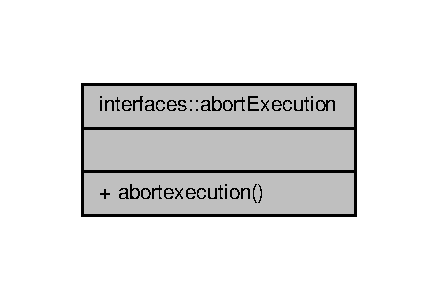
\includegraphics[width=210pt]{interfaceinterfaces_1_1abort_execution__coll__graph}
\end{center}
\end{figure}
\subsection*{Public Member Functions}
\begin{DoxyCompactItemize}
\item 
subroutine \hyperlink{interfaceinterfaces_1_1abort_execution_a80e28af83055359ee64f57fb1a7fa48b}{abortexecution} (i, j, line, word, r1, r2, i\-Vec)
\end{DoxyCompactItemize}


\subsection{Detailed Description}


Definition at line 38 of file interfaces.\-f90.



\subsection{Member Function/\-Subroutine Documentation}
\hypertarget{interfaceinterfaces_1_1abort_execution_a80e28af83055359ee64f57fb1a7fa48b}{\index{interfaces\-::abort\-Execution@{interfaces\-::abort\-Execution}!abortexecution@{abortexecution}}
\index{abortexecution@{abortexecution}!interfaces::abortExecution@{interfaces\-::abort\-Execution}}
\subsubsection[{abortexecution}]{\setlength{\rightskip}{0pt plus 5cm}subroutine interfaces\-::abort\-Execution\-::abortexecution (
\begin{DoxyParamCaption}
\item[{integer, intent(in), optional}]{i, }
\item[{integer, intent(in), optional}]{j, }
\item[{integer, intent(in), optional}]{line, }
\item[{character(len=$\ast$), intent(in), optional}]{word, }
\item[{real(kind = prec), intent(in), optional}]{r1, }
\item[{real(kind = prec), intent(in), optional}]{r2, }
\item[{real(kind = prec), dimension($\ast$), intent(in), optional}]{i\-Vec}
\end{DoxyParamCaption}
)}}\label{interfaceinterfaces_1_1abort_execution_a80e28af83055359ee64f57fb1a7fa48b}


Definition at line 38 of file interfaces.\-f90.



The documentation for this interface was generated from the following file\-:\begin{DoxyCompactItemize}
\item 
/home/\-Progetti/\-Siat/\-Ottimizzatore/src/\hyperlink{interfaces_8f90}{interfaces.\-f90}\end{DoxyCompactItemize}

\hypertarget{interfacefiletools_1_1c_find_entry}{\section{filetools\-:\-:c\-Find\-Entry Interface Reference}
\label{interfacefiletools_1_1c_find_entry}\index{filetools\-::c\-Find\-Entry@{filetools\-::c\-Find\-Entry}}
}


Collaboration diagram for filetools\-:\-:c\-Find\-Entry\-:\nopagebreak
\begin{figure}[H]
\begin{center}
\leavevmode
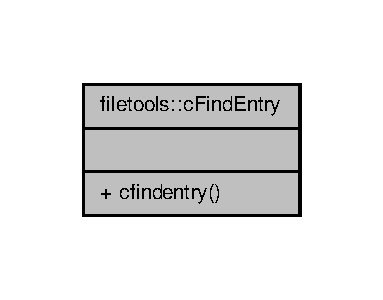
\includegraphics[width=184pt]{interfacefiletools_1_1c_find_entry__coll__graph}
\end{center}
\end{figure}
\subsection*{Public Member Functions}
\begin{DoxyCompactItemize}
\item 
subroutine \hyperlink{interfacefiletools_1_1c_find_entry_af8f083dc5d82069ac9c02e3ae98e30bf}{cfindentry} (entry, n, the\-Unit, rew, valore, is\-Present, n\-Row)
\end{DoxyCompactItemize}


\subsection{Detailed Description}


Definition at line 139 of file file\-Tools.\-f90.



\subsection{Member Function/\-Subroutine Documentation}
\hypertarget{interfacefiletools_1_1c_find_entry_af8f083dc5d82069ac9c02e3ae98e30bf}{\index{filetools\-::c\-Find\-Entry@{filetools\-::c\-Find\-Entry}!cfindentry@{cfindentry}}
\index{cfindentry@{cfindentry}!filetools::cFindEntry@{filetools\-::c\-Find\-Entry}}
\subsubsection[{cfindentry}]{\setlength{\rightskip}{0pt plus 5cm}subroutine filetools\-::c\-Find\-Entry\-::cfindentry (
\begin{DoxyParamCaption}
\item[{character(len=$\ast$), intent(in)}]{entry, }
\item[{integer, intent(in)}]{n, }
\item[{integer, intent(in)}]{the\-Unit, }
\item[{logical, intent(in), optional}]{rew, }
\item[{character(len=100), dimension(n), intent(out), optional}]{valore, }
\item[{logical, intent(out), optional}]{is\-Present, }
\item[{integer, intent(out), optional}]{n\-Row}
\end{DoxyParamCaption}
)}}\label{interfacefiletools_1_1c_find_entry_af8f083dc5d82069ac9c02e3ae98e30bf}


Definition at line 139 of file file\-Tools.\-f90.



The documentation for this interface was generated from the following file\-:\begin{DoxyCompactItemize}
\item 
/home/\-Progetti/\-Siat/\-Ottimizzatore/src/\hyperlink{file_tools_8f90}{file\-Tools.\-f90}\end{DoxyCompactItemize}

\hypertarget{interfacefiletools_1_1c_matrix_read}{\section{filetools\-:\-:c\-Matrix\-Read Interface Reference}
\label{interfacefiletools_1_1c_matrix_read}\index{filetools\-::c\-Matrix\-Read@{filetools\-::c\-Matrix\-Read}}
}


Collaboration diagram for filetools\-:\-:c\-Matrix\-Read\-:\nopagebreak
\begin{figure}[H]
\begin{center}
\leavevmode
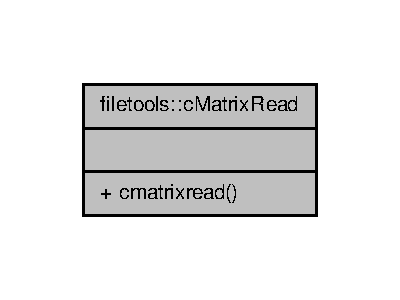
\includegraphics[width=192pt]{interfacefiletools_1_1c_matrix_read__coll__graph}
\end{center}
\end{figure}
\subsection*{Public Member Functions}
\begin{DoxyCompactItemize}
\item 
character(len=100) function, \\*
dimension(nline, ncol) \hyperlink{interfacefiletools_1_1c_matrix_read_ad46208c86143112574df85f78b52bc95}{cmatrixread} (the\-Unit, nline, ncol, first\-\_\-, last\-\_\-)
\end{DoxyCompactItemize}


\subsection{Detailed Description}


Definition at line 84 of file file\-Tools.\-f90.



\subsection{Member Function/\-Subroutine Documentation}
\hypertarget{interfacefiletools_1_1c_matrix_read_ad46208c86143112574df85f78b52bc95}{\index{filetools\-::c\-Matrix\-Read@{filetools\-::c\-Matrix\-Read}!cmatrixread@{cmatrixread}}
\index{cmatrixread@{cmatrixread}!filetools::cMatrixRead@{filetools\-::c\-Matrix\-Read}}
\subsubsection[{cmatrixread}]{\setlength{\rightskip}{0pt plus 5cm}character(len=100) function, dimension(nline,ncol) filetools\-::c\-Matrix\-Read\-::cmatrixread (
\begin{DoxyParamCaption}
\item[{integer, intent(in)}]{the\-Unit, }
\item[{integer, intent(in)}]{nline, }
\item[{integer, intent(in)}]{ncol, }
\item[{character(len=1), optional}]{first\-\_\-, }
\item[{character(len=1), optional}]{last\-\_\-}
\end{DoxyParamCaption}
)}}\label{interfacefiletools_1_1c_matrix_read_ad46208c86143112574df85f78b52bc95}


Definition at line 84 of file file\-Tools.\-f90.



The documentation for this interface was generated from the following file\-:\begin{DoxyCompactItemize}
\item 
/home/andrea/\-Desktop/\-Fortran\-Code\-B\-W/src/\hyperlink{file_tools_8f90}{file\-Tools.\-f90}\end{DoxyCompactItemize}

\hypertarget{classcmdvar}{\section{cmdvar Module Reference}
\label{classcmdvar}\index{cmdvar@{cmdvar}}
}


Collects the variable read from command line.  




Collaboration diagram for cmdvar\-:\nopagebreak
\begin{figure}[H]
\begin{center}
\leavevmode
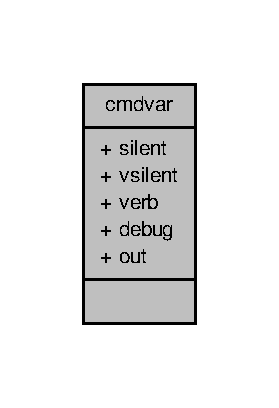
\includegraphics[width=134pt]{classcmdvar__coll__graph}
\end{center}
\end{figure}
\subsection*{Public Attributes}
\begin{DoxyCompactItemize}
\item 
logical \hyperlink{classcmdvar_a774f2caff8f9563a52b69cf5c205da28}{silent}
\begin{DoxyCompactList}\small\item\em Controls the input to the screen. \end{DoxyCompactList}\item 
logical \hyperlink{classcmdvar_a5d5ef4d5f7d8f3ec8c8e390e0f594ec1}{vsilent}
\item 
logical \hyperlink{classcmdvar_ab46a1faddb3f0a3fe76bfa461154ffcc}{verb}
\item 
logical \hyperlink{classcmdvar_a040fa7b1b07323379cfc623dbf43d7c0}{debug}
\item 
character(len=100) \hyperlink{classcmdvar_aa24632df9762e42214c48cd1f53bb6e3}{out}
\end{DoxyCompactItemize}


\subsection{Detailed Description}
Collects the variable read from command line. \begin{DoxyAuthor}{Author}
Andrea Facci 
\end{DoxyAuthor}


Definition at line 39 of file cmd\-Var.\-f90.



\subsection{Member Data Documentation}
\hypertarget{classcmdvar_a040fa7b1b07323379cfc623dbf43d7c0}{\index{cmdvar@{cmdvar}!debug@{debug}}
\index{debug@{debug}!cmdvar@{cmdvar}}
\subsubsection[{debug}]{\setlength{\rightskip}{0pt plus 5cm}logical cmdvar\-::debug}}\label{classcmdvar_a040fa7b1b07323379cfc623dbf43d7c0}


Definition at line 42 of file cmd\-Var.\-f90.

\hypertarget{classcmdvar_aa24632df9762e42214c48cd1f53bb6e3}{\index{cmdvar@{cmdvar}!out@{out}}
\index{out@{out}!cmdvar@{cmdvar}}
\subsubsection[{out}]{\setlength{\rightskip}{0pt plus 5cm}character(len=100) cmdvar\-::out}}\label{classcmdvar_aa24632df9762e42214c48cd1f53bb6e3}


Definition at line 43 of file cmd\-Var.\-f90.

\hypertarget{classcmdvar_a774f2caff8f9563a52b69cf5c205da28}{\index{cmdvar@{cmdvar}!silent@{silent}}
\index{silent@{silent}!cmdvar@{cmdvar}}
\subsubsection[{silent}]{\setlength{\rightskip}{0pt plus 5cm}logical cmdvar\-::silent}}\label{classcmdvar_a774f2caff8f9563a52b69cf5c205da28}


Definition at line 42 of file cmd\-Var.\-f90.

\hypertarget{classcmdvar_ab46a1faddb3f0a3fe76bfa461154ffcc}{\index{cmdvar@{cmdvar}!verb@{verb}}
\index{verb@{verb}!cmdvar@{cmdvar}}
\subsubsection[{verb}]{\setlength{\rightskip}{0pt plus 5cm}logical cmdvar\-::verb}}\label{classcmdvar_ab46a1faddb3f0a3fe76bfa461154ffcc}


Definition at line 42 of file cmd\-Var.\-f90.

\hypertarget{classcmdvar_a5d5ef4d5f7d8f3ec8c8e390e0f594ec1}{\index{cmdvar@{cmdvar}!vsilent@{vsilent}}
\index{vsilent@{vsilent}!cmdvar@{cmdvar}}
\subsubsection[{vsilent}]{\setlength{\rightskip}{0pt plus 5cm}logical cmdvar\-::vsilent}}\label{classcmdvar_a5d5ef4d5f7d8f3ec8c8e390e0f594ec1}


Definition at line 42 of file cmd\-Var.\-f90.



The documentation for this module was generated from the following file\-:\begin{DoxyCompactItemize}
\item 
/home/\-Codici/\-Blink/\-Power\-Manager/src/\hyperlink{cmd_var_8f90}{cmd\-Var.\-f90}\end{DoxyCompactItemize}

\hypertarget{interfacegraphtools_1_1constraints}{\section{graphtools\-:\-:constraints Interface Reference}
\label{interfacegraphtools_1_1constraints}\index{graphtools\-::constraints@{graphtools\-::constraints}}
}


Collaboration diagram for graphtools\-:\-:constraints\-:\nopagebreak
\begin{figure}[H]
\begin{center}
\leavevmode
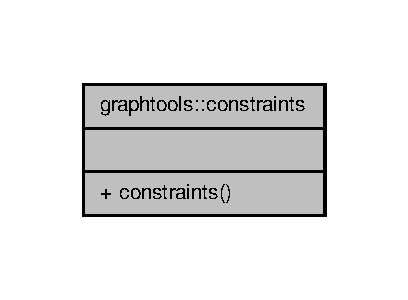
\includegraphics[width=196pt]{interfacegraphtools_1_1constraints__coll__graph}
\end{center}
\end{figure}
\subsection*{Public Member Functions}
\begin{DoxyCompactItemize}
\item 
logical function \hyperlink{interfacegraphtools_1_1constraints_ac9d0e4805d083cf1018e385898c7fe5f}{constraints} (c, t)
\end{DoxyCompactItemize}


\subsection{Detailed Description}


Definition at line 67 of file graph\-Tools.\-f90.



\subsection{Constructor \& Destructor Documentation}
\hypertarget{interfacegraphtools_1_1constraints_ac9d0e4805d083cf1018e385898c7fe5f}{\index{graphtools\-::constraints@{graphtools\-::constraints}!constraints@{constraints}}
\index{constraints@{constraints}!graphtools::constraints@{graphtools\-::constraints}}
\subsubsection[{constraints}]{\setlength{\rightskip}{0pt plus 5cm}logical function graphtools\-::constraints\-::constraints (
\begin{DoxyParamCaption}
\item[{integer, dimension(nm), intent(in)}]{c, }
\item[{integer, intent(in)}]{t}
\end{DoxyParamCaption}
)}}\label{interfacegraphtools_1_1constraints_ac9d0e4805d083cf1018e385898c7fe5f}


Definition at line 67 of file graph\-Tools.\-f90.



The documentation for this interface was generated from the following file\-:\begin{DoxyCompactItemize}
\item 
/home/andrea/\-Desktop/\-Fortran\-Code\-B\-W/src/\hyperlink{graph_tools_8f90}{graph\-Tools.\-f90}\end{DoxyCompactItemize}

\hypertarget{interfacefiletools_1_1d_find_entry}{\section{filetools\-:\-:d\-Find\-Entry Interface Reference}
\label{interfacefiletools_1_1d_find_entry}\index{filetools\-::d\-Find\-Entry@{filetools\-::d\-Find\-Entry}}
}


Collaboration diagram for filetools\-:\-:d\-Find\-Entry\-:\nopagebreak
\begin{figure}[H]
\begin{center}
\leavevmode
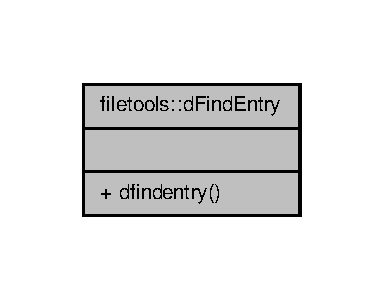
\includegraphics[width=184pt]{interfacefiletools_1_1d_find_entry__coll__graph}
\end{center}
\end{figure}
\subsection*{Public Member Functions}
\begin{DoxyCompactItemize}
\item 
subroutine \hyperlink{interfacefiletools_1_1d_find_entry_a5ec867262eca2566d523b83684eb69fa}{dfindentry} (entry, n, the\-Unit, rew, valore, is\-Present, n\-Row)
\end{DoxyCompactItemize}


\subsection{Detailed Description}


Definition at line 125 of file file\-Tools.\-f90.



\subsection{Member Function/\-Subroutine Documentation}
\hypertarget{interfacefiletools_1_1d_find_entry_a5ec867262eca2566d523b83684eb69fa}{\index{filetools\-::d\-Find\-Entry@{filetools\-::d\-Find\-Entry}!dfindentry@{dfindentry}}
\index{dfindentry@{dfindentry}!filetools::dFindEntry@{filetools\-::d\-Find\-Entry}}
\subsubsection[{dfindentry}]{\setlength{\rightskip}{0pt plus 5cm}subroutine filetools\-::d\-Find\-Entry\-::dfindentry (
\begin{DoxyParamCaption}
\item[{character(len=$\ast$), intent(in)}]{entry, }
\item[{integer, intent(in)}]{n, }
\item[{integer, intent(in)}]{the\-Unit, }
\item[{logical, intent(in), optional}]{rew, }
\item[{real(kind = prec), dimension(n), intent(out), optional}]{valore, }
\item[{logical, intent(out), optional}]{is\-Present, }
\item[{integer, intent(out), optional}]{n\-Row}
\end{DoxyParamCaption}
)}}\label{interfacefiletools_1_1d_find_entry_a5ec867262eca2566d523b83684eb69fa}


Definition at line 125 of file file\-Tools.\-f90.



The documentation for this interface was generated from the following file\-:\begin{DoxyCompactItemize}
\item 
/home/\-Codici/\-Blink/\-Power\-Manager/src/\hyperlink{file_tools_8f90}{file\-Tools.\-f90}\end{DoxyCompactItemize}

\hypertarget{interfacefiletools_1_1d_matrix_read}{\section{filetools\-:\-:d\-Matrix\-Read Interface Reference}
\label{interfacefiletools_1_1d_matrix_read}\index{filetools\-::d\-Matrix\-Read@{filetools\-::d\-Matrix\-Read}}
}


Collaboration diagram for filetools\-:\-:d\-Matrix\-Read\-:\nopagebreak
\begin{figure}[H]
\begin{center}
\leavevmode
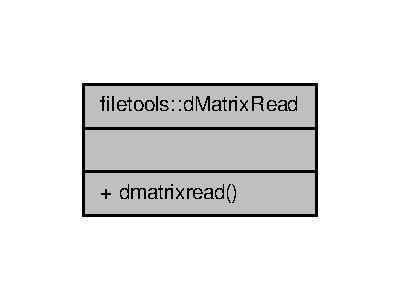
\includegraphics[width=192pt]{interfacefiletools_1_1d_matrix_read__coll__graph}
\end{center}
\end{figure}
\subsection*{Public Member Functions}
\begin{DoxyCompactItemize}
\item 
real(kind(1.d0)) function, \\*
dimension(nline, ncol) \hyperlink{interfacefiletools_1_1d_matrix_read_ade43d60737b02be7730f15a6cdf20b83}{dmatrixread} (the\-Unit, nline, ncol, first\-\_\-, last\-\_\-)
\end{DoxyCompactItemize}


\subsection{Detailed Description}


Definition at line 66 of file file\-Tools.\-f90.



\subsection{Member Function/\-Subroutine Documentation}
\hypertarget{interfacefiletools_1_1d_matrix_read_ade43d60737b02be7730f15a6cdf20b83}{\index{filetools\-::d\-Matrix\-Read@{filetools\-::d\-Matrix\-Read}!dmatrixread@{dmatrixread}}
\index{dmatrixread@{dmatrixread}!filetools::dMatrixRead@{filetools\-::d\-Matrix\-Read}}
\subsubsection[{dmatrixread}]{\setlength{\rightskip}{0pt plus 5cm}real(kind(1.d0)) function, dimension(nline,ncol) filetools\-::d\-Matrix\-Read\-::dmatrixread (
\begin{DoxyParamCaption}
\item[{integer, intent(in)}]{the\-Unit, }
\item[{integer, intent(in)}]{nline, }
\item[{integer, intent(in)}]{ncol, }
\item[{character(len=1), optional}]{first\-\_\-, }
\item[{character(len=1), optional}]{last\-\_\-}
\end{DoxyParamCaption}
)}}\label{interfacefiletools_1_1d_matrix_read_ade43d60737b02be7730f15a6cdf20b83}


Definition at line 66 of file file\-Tools.\-f90.



The documentation for this interface was generated from the following file\-:\begin{DoxyCompactItemize}
\item 
/home/andrea/\-Desktop/\-Fortran\-Code\-B\-W/src/\hyperlink{file_tools_8f90}{file\-Tools.\-f90}\end{DoxyCompactItemize}

\hypertarget{classeconomy}{\section{economy Module Reference}
\label{classeconomy}\index{economy@{economy}}
}


Collaboration diagram for economy\-:\nopagebreak
\begin{figure}[H]
\begin{center}
\leavevmode
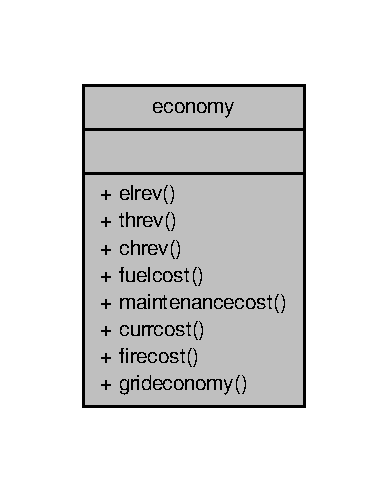
\includegraphics[width=186pt]{classeconomy__coll__graph}
\end{center}
\end{figure}
\subsection*{Public Member Functions}
\begin{DoxyCompactItemize}
\item 
real(kind=prec) function \hyperlink{classeconomy_a4ab4325ba4da5a36bfc71dad24b101c6}{elrev} (c, t)
\begin{DoxyCompactList}\small\item\em Electric energy revenues. \end{DoxyCompactList}\item 
real(kind=prec) function \hyperlink{classeconomy_a5f12114d9d3d02f2d9590df75c787003}{threv} (t)
\begin{DoxyCompactList}\small\item\em thermal energy revenues. \end{DoxyCompactList}\item 
real(kind=prec) function \hyperlink{classeconomy_af1f82a2c63a713af1676de7fb05aadc5}{chrev} (t)
\begin{DoxyCompactList}\small\item\em Chilling energy revenues. \end{DoxyCompactList}\item 
real(kind=prec) function \hyperlink{classeconomy_aa8f3af6fe0e525bc72f54bf369789443}{fuelcost} (c, t)
\begin{DoxyCompactList}\small\item\em Calculates the costs to buy the fuel. \end{DoxyCompactList}\item 
real(kind=prec) function \hyperlink{classeconomy_af6ed48a60d50c438efa98f16deed7520}{maintenancecost} (c, t)
\begin{DoxyCompactList}\small\item\em Calculates the mintenance costs. \end{DoxyCompactList}\item 
real(kind=prec) function \hyperlink{classeconomy_a542c71f53d112855d6a81bf21941c8a9}{currcost} (c, t)
\begin{DoxyCompactList}\small\item\em Calculates the profit during a time step. \end{DoxyCompactList}\item 
real(kind=prec) function \hyperlink{classeconomy_ace504d2735fcf5bab047994e760346a9}{firecost} (c\-New, c\-Old)
\begin{DoxyCompactList}\small\item\em Calculates the lighting cost. \end{DoxyCompactList}\item 
real(kind=prec) function, \\*
dimension(2) \hyperlink{classeconomy_a47cc446e4047749cb8b4ae10372ae3c4}{grideconomy} (c, t)
\end{DoxyCompactItemize}


\subsection{Detailed Description}
\begin{DoxyAuthor}{Author}

\end{DoxyAuthor}
This module contains the definition of all the procedures that perform economic calculations for a give set-\/point and time-\/step, that are, fuel costs, O\&M costs, and the revenues from thermal, electric, and chilling, energy selling. \begin{DoxyAuthor}{Author}

\end{DoxyAuthor}


Definition at line 44 of file economy.\-f90.



\subsection{Member Function/\-Subroutine Documentation}
\hypertarget{classeconomy_af1f82a2c63a713af1676de7fb05aadc5}{\index{economy@{economy}!chrev@{chrev}}
\index{chrev@{chrev}!economy@{economy}}
\subsubsection[{chrev}]{\setlength{\rightskip}{0pt plus 5cm}real(kind = prec) function economy\-::chrev (
\begin{DoxyParamCaption}
\item[{integer, intent(in)}]{t}
\end{DoxyParamCaption}
)}}\label{classeconomy_af1f82a2c63a713af1676de7fb05aadc5}
Calculates the revenues (in euro or any other currency according to the one used in the input) from chilling energy selling to the various clients. \[ R_{ch} = \sum_{clients} U_{ch}(i)c_{ch}(i)dt \] where $ U_{ch}(i)$ is the power demand (in k\-W) of the $i$'th client, $c_{ch}(i)$ is the price in euro/k\-J of electric energy for each client and $ dt$ is the time-\/step duration.\par
 
\begin{DoxyParams}[1]{Parameters}
\mbox{\tt in}  & {\em c} & index of the given set-\/point to be given as input. Defines the state of the plant $sp(i) = sp(c\_(i))$ \\
\hline
\mbox{\tt in}  & {\em t} & time step index. Note t=x meas the x'th time step from the simulation start. \\
\hline
\end{DoxyParams}
\begin{DoxyAuthor}{Author}
Andrea Facci 
\end{DoxyAuthor}


Definition at line 187 of file economy.\-f90.



Referenced by currcost(), and globalresults\-::globchrev().

\hypertarget{classeconomy_a542c71f53d112855d6a81bf21941c8a9}{\index{economy@{economy}!currcost@{currcost}}
\index{currcost@{currcost}!economy@{economy}}
\subsubsection[{currcost}]{\setlength{\rightskip}{0pt plus 5cm}real(kind = prec) function economy\-::currcost (
\begin{DoxyParamCaption}
\item[{integer, dimension(nm), intent(in)}]{c, }
\item[{integer, intent(in)}]{t}
\end{DoxyParamCaption}
)}}\label{classeconomy_a542c71f53d112855d6a81bf21941c8a9}
Calculates the profit of a time-\/step(in euro or any other currency according to the one used in the input) for a given set-\/point, all the costs, except for the costs associated to equipment ignition. \[ G = R_{el} + R_{th} + R_{ch} + C_{f} + C_{m} \] where \par

\begin{DoxyItemize}
\item $R_{el}$ are the electrical revenues;
\item $R_{th}$ are the thermal revenues;
\item $R_{ch}$ are the chilling revenues
\item $C_{f}$ are the fuel costs;
\item $C_{m}$ are the maintenance costs;
\item $ dt$ is the time-\/step duration.\par
 Having discarded lighting costs, this profit depends only on the state of the plant at a determined time-\/step and not on the state at pre previous or subsequent time-\/step and will be associated to a vertex of the graph. 
\begin{DoxyParams}[1]{Parameters}
\mbox{\tt in}  & {\em c} & index of the given set-\/point to be given as input. Defines the state of the plant $sp(i) = sp(c\_(i))$ \\
\hline
\mbox{\tt in}  & {\em t} & time step index. Note t=x meas the x'th time step from the simulation start. \\
\hline
\end{DoxyParams}
\begin{DoxyAuthor}{Author}
Andrea Facci 
\end{DoxyAuthor}

\end{DoxyItemize}

Definition at line 322 of file economy.\-f90.



References chrev(), elrev(), fuelcost(), maintenancecost(), and threv().



Referenced by objfunction().

\hypertarget{classeconomy_a4ab4325ba4da5a36bfc71dad24b101c6}{\index{economy@{economy}!elrev@{elrev}}
\index{elrev@{elrev}!economy@{economy}}
\subsubsection[{elrev}]{\setlength{\rightskip}{0pt plus 5cm}real(kind = prec) function economy\-::elrev (
\begin{DoxyParamCaption}
\item[{integer, dimension(nm), intent(in)}]{c, }
\item[{integer, intent(in)}]{t}
\end{DoxyParamCaption}
)}}\label{classeconomy_a4ab4325ba4da5a36bfc71dad24b101c6}
Calculates the revenues (in euro or any other currency according to the one used in the input) from electric energy selling to the various clients and to the grid. Electric energy revenues are calculated in a different way for each kind of grid connection. Specifically\-:\par

\begin{DoxyItemize}
\item Stand Alone\-: \[ R_{el} = \sum_{clients} U_{el}(i)c_{el}(i)dt \] where $ U_{el}(i)$ is the power demand (in k\-W) of the $i$'th client, $c_{el}(i)$ is the price in euro/k\-J of electric energy for each client and $ dt$ is the time-\/step duration.\par

\item Grid connected with net metering\-: \[ R_{el} = \sum_{clients} U_{el}(i)c_{el}(i)dt + P_{el}c_{s_{grid}} - U_{el}^{t}c_{b_{grid}} \] where $P_{el}$ is the total electric power produced by the power plant, $c_{s_{grid}}$ is the selling price to the grid, $U_{el}^{t} = \sum_{clients} U_{el}(i) + U_{el}^{self} $ is the total electric demand, including the power plant self-\/consumption $U_{el}^{self}$\par

\item Grid Connected without net metering\-: \[ R_{el} = \sum_{clients} U_{el}(i)c_{el}(i)dt + (P_{el} - U_{el}^{t}) c_{grid} \] where $ c_{grid} = c_{s_{grid}}$ if $P_{el} \ge U_{el}^{t}$ and $ c_{grid} = c_{b_{grid}}$ otherwise 
\begin{DoxyParams}[1]{Parameters}
\mbox{\tt in}  & {\em c} & index of the given set-\/point to be given as input. Defines the state of the plant $sp(i) = sp(c\_(i))$ \\
\hline
\mbox{\tt in}  & {\em t} & time step index. Note t=x meas the x'th time step from the simulation start. \\
\hline
\end{DoxyParams}
\begin{DoxyAuthor}{Author}
Andrea Facci 
\end{DoxyAuthor}

\end{DoxyItemize}

Definition at line 80 of file economy.\-f90.



References energy\-::elprod(), and energy\-::elselfcons().



Referenced by currcost(), and globalresults\-::globelrev().

\hypertarget{classeconomy_ace504d2735fcf5bab047994e760346a9}{\index{economy@{economy}!firecost@{firecost}}
\index{firecost@{firecost}!economy@{economy}}
\subsubsection[{firecost}]{\setlength{\rightskip}{0pt plus 5cm}real(kind = prec) function economy\-::firecost (
\begin{DoxyParamCaption}
\item[{integer, dimension(nm), intent(in)}]{c\-New, }
\item[{integer, dimension(nm), intent(in)}]{c\-Old}
\end{DoxyParamCaption}
)}}\label{classeconomy_ace504d2735fcf5bab047994e760346a9}
Calculates the cost associated to each lighting of a machinery. \[ C_{l} > 0 \qquad \mbox{if} \qquad sp(t,i) > 0 \;\mbox{and}\; sp(t-1,i) = 0 \] this cost will be added to the operative profit to for the arc profit/cost. 
\begin{DoxyParams}[1]{Parameters}
\mbox{\tt in}  & {\em c} & index of the given set-\/point to be given as input. Defines the state of the plant $sp(i) = sp(c\_(i))$ \\
\hline
\mbox{\tt in}  & {\em t} & time step index. Note t=x meas the x'th time step from the simulation start. \\
\hline
\end{DoxyParams}
\begin{DoxyAuthor}{Author}
Andrea Facci 
\end{DoxyAuthor}


Definition at line 355 of file economy.\-f90.



Referenced by globalresults\-::globfirecost(), graphtools\-::grapharcs(), and output().

\hypertarget{classeconomy_aa8f3af6fe0e525bc72f54bf369789443}{\index{economy@{economy}!fuelcost@{fuelcost}}
\index{fuelcost@{fuelcost}!economy@{economy}}
\subsubsection[{fuelcost}]{\setlength{\rightskip}{0pt plus 5cm}real(kind = prec) function economy\-::fuelcost (
\begin{DoxyParamCaption}
\item[{integer, dimension(nm), intent(in)}]{c, }
\item[{integer, intent(in)}]{t}
\end{DoxyParamCaption}
)}}\label{classeconomy_aa8f3af6fe0e525bc72f54bf369789443}
Calculates the costs to buy the fuel (in euro or any other currency according to the one used in the input) \[ C_{f} = \sum_{Trig+Boi} \frac{E_{in}(i)c_{f}(i)}{H_i(i)}dt \] where $c_{f}(i)$ is the specific cost (per unit mass or volume) of the fuel for the $i$'th machine, $H_i(i)$ is the fuel L\-H\-V (k\-J per unit mass or volume), $E_{in}(i)$ is the primary energy input. $c_{ch}(i)$ is the price in euro/k\-J of electric energy for each client and $ dt$ is the time-\/step duration.\par
 Note that even though international units are strongly suggested, any units of mass and/or volume is valid for $c_{f}$ and $H_i$ provided that coherence between the units of these two variables is respected. Moreover prices and L\-V\-Ss may may be expressend in different units for differend machines. 
\begin{DoxyParams}[1]{Parameters}
\mbox{\tt in}  & {\em c} & index of the given set-\/point to be given as input. Defines the state of the plant $sp(i) = sp(c\_(i))$ \\
\hline
\mbox{\tt in}  & {\em t} & time step index. Note t=x meas the x'th time step from the simulation start. \\
\hline
\end{DoxyParams}
\begin{DoxyAuthor}{Author}
Andrea Facci 
\end{DoxyAuthor}


Definition at line 233 of file economy.\-f90.



References energy\-::fuelcons().



Referenced by currcost(), globalresults\-::globfuelcost(), and output().

\hypertarget{classeconomy_a47cc446e4047749cb8b4ae10372ae3c4}{\index{economy@{economy}!grideconomy@{grideconomy}}
\index{grideconomy@{grideconomy}!economy@{economy}}
\subsubsection[{grideconomy}]{\setlength{\rightskip}{0pt plus 5cm}real(kind = prec) function, dimension(2) economy\-::grideconomy (
\begin{DoxyParamCaption}
\item[{integer, dimension(nm), intent(in)}]{c, }
\item[{integer, intent(in)}]{t}
\end{DoxyParamCaption}
)}}\label{classeconomy_a47cc446e4047749cb8b4ae10372ae3c4}


Definition at line 380 of file economy.\-f90.



References energy\-::elprod(), and energy\-::elselfcons().



Referenced by output().

\hypertarget{classeconomy_af6ed48a60d50c438efa98f16deed7520}{\index{economy@{economy}!maintenancecost@{maintenancecost}}
\index{maintenancecost@{maintenancecost}!economy@{economy}}
\subsubsection[{maintenancecost}]{\setlength{\rightskip}{0pt plus 5cm}real(kind = prec) function economy\-::maintenancecost (
\begin{DoxyParamCaption}
\item[{integer, dimension(nm), intent(in)}]{c, }
\item[{integer, intent(in)}]{t}
\end{DoxyParamCaption}
)}}\label{classeconomy_af6ed48a60d50c438efa98f16deed7520}
Calculates the maintenance costs (in euro or any other currency according to the one used in the input) \[ C_{m} = \sum c_{m}(i)dt \qquad \mbox{if}\qquad sp(i) > 0 \] where $c_{m}(i)$ is the maintenance cost per unit time and $ dt$ is the time-\/step duration.\par
 
\begin{DoxyParams}[1]{Parameters}
\mbox{\tt in}  & {\em c} & index of the given set-\/point to be given as input. Defines the state of the plant $sp(i) = sp(c\_(i))$ \\
\hline
\mbox{\tt in}  & {\em t} & time step index. Note t=x meas the x'th time step from the simulation start. \\
\hline
\end{DoxyParams}
\begin{DoxyAuthor}{Author}
Andrea Facci 
\end{DoxyAuthor}


Definition at line 276 of file economy.\-f90.



Referenced by currcost(), globalresults\-::globmaintcost(), and output().

\hypertarget{classeconomy_a5f12114d9d3d02f2d9590df75c787003}{\index{economy@{economy}!threv@{threv}}
\index{threv@{threv}!economy@{economy}}
\subsubsection[{threv}]{\setlength{\rightskip}{0pt plus 5cm}real(kind = prec) function economy\-::threv (
\begin{DoxyParamCaption}
\item[{integer, intent(in)}]{t}
\end{DoxyParamCaption}
)}}\label{classeconomy_a5f12114d9d3d02f2d9590df75c787003}
Calculates the revenues (in euro or any other currency according to the one used in the input) from thermal energy selling to the various clients. \[ R_{th} = \sum_{clients} U_{th}(i)c_{th}(i)dt \] where $ U_{th}(i)$ is the power demand (in k\-W) of the $i$'th client, $c_{th}(i)$ is the price in euro/k\-J of electric energy for each client and $ dt$ is the time-\/step duration.\par
 
\begin{DoxyParams}[1]{Parameters}
\mbox{\tt in}  & {\em c} & index of the given set-\/point to be given as input. Defines the state of the plant $sp(i) = sp(c\_(i))$ \\
\hline
\mbox{\tt in}  & {\em t} & time step index. Note t=x meas the x'th time step from the simulation start. \\
\hline
\end{DoxyParams}
\begin{DoxyAuthor}{Author}
Andrea Facci 
\end{DoxyAuthor}


Definition at line 147 of file economy.\-f90.



Referenced by currcost(), and globalresults\-::globthrev().



The documentation for this module was generated from the following file\-:\begin{DoxyCompactItemize}
\item 
/home/\-Codici/\-Blink/\-Power\-Manager/src/\hyperlink{economy_8f90}{economy.\-f90}\end{DoxyCompactItemize}

\hypertarget{classenergy}{\section{energy Module Reference}
\label{classenergy}\index{energy@{energy}}
}


module for energy calculations.  




Collaboration diagram for energy\-:\nopagebreak
\begin{figure}[H]
\begin{center}
\leavevmode
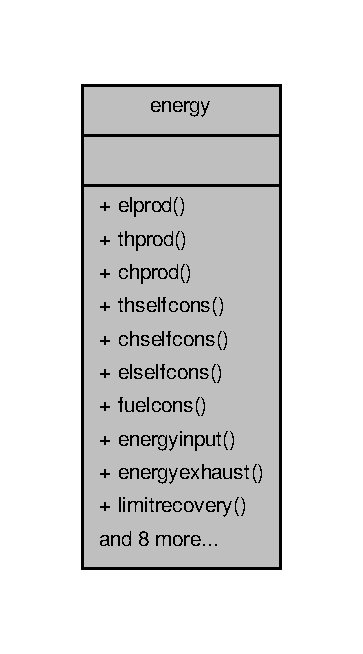
\includegraphics[width=174pt]{classenergy__coll__graph}
\end{center}
\end{figure}
\subsection*{Public Member Functions}
\begin{DoxyCompactItemize}
\item 
real(kind=prec) function \hyperlink{classenergy_a5ce8ae58805b4f7abe840bedaea30a00}{elprod} (c\-\_\-, t)
\begin{DoxyCompactList}\small\item\em Electrical production. \end{DoxyCompactList}\item 
real(kind=prec) function \hyperlink{classenergy_a40ddda3c07be743826be8c2e982b9b98}{thprod} (c\-\_\-, t)
\begin{DoxyCompactList}\small\item\em Thermal production. \end{DoxyCompactList}\item 
real(kind=prec) function \hyperlink{classenergy_a78e3e5b7396e41d13b3c9aa8f4edca48}{chprod} (c\-\_\-, t)
\begin{DoxyCompactList}\small\item\em Chilling production. \end{DoxyCompactList}\item 
real(kind=prec) function \hyperlink{classenergy_af385040819d802e1a3c9e0c9a692ff0a}{thselfcons} (c\-\_\-, t)
\begin{DoxyCompactList}\small\item\em Internal thermal consumption of the power plant. \end{DoxyCompactList}\item 
real(kind=prec) function \hyperlink{classenergy_af5299e75015a3803765a6b49efa22049}{elselfcons} (c\-\_\-, t)
\begin{DoxyCompactList}\small\item\em Internal electrical consumption of the power plant. \end{DoxyCompactList}\item 
real(kind=prec) function, \\*
dimension(nboi+ntrig) \hyperlink{classenergy_a07a977e68ea1d19da65ba06a4e4007a2}{fuelcons} (c\-\_\-, t)
\begin{DoxyCompactList}\small\item\em Primary energy input. \end{DoxyCompactList}\item 
real(kind=prec) function, \\*
dimension(nm) \hyperlink{classenergy_aebd116fdbb931db63a6450c7ba3197df}{energyinput} (c\-\_\-, t)
\begin{DoxyCompactList}\small\item\em Primary energy input. \end{DoxyCompactList}\item 
real(kind=prec) function, \\*
dimension(ntrig+nboi) \hyperlink{classenergy_aa9595768898cb233d53596e9ce19744f}{energyexhaust} (c\-\_\-, t)
\begin{DoxyCompactList}\small\item\em Energy exhausted by combustions equipment. \end{DoxyCompactList}\item 
real(kind=prec) function \hyperlink{classenergy_adee2b0ef7e3ae6a8da4a2357ffa14a28}{limitrecovery} (i, valore, t)
\begin{DoxyCompactList}\small\item\em Limit the power of an H\-R\-S\-G. \end{DoxyCompactList}\item 
real(kind=prec) function \hyperlink{classenergy_a6060381a3418f406c8ca108f9c5a7fd5}{cogthprod} (c\-\_\-, t)
\begin{DoxyCompactList}\small\item\em Cogenerative Thermal production. \end{DoxyCompactList}\item 
real(kind=prec) function \hyperlink{classenergy_a082e1efb7fb9b51f62cfe800fefe1585}{pec} (c, t)
\begin{DoxyCompactList}\small\item\em Primary Energy Consumption. \end{DoxyCompactList}\item 
real(kind=prec) function \hyperlink{classenergy_a85b1719a96ad6c8ccc87e720cb6b0397}{pecpenalty} (c\-New, c\-Old, t)
\begin{DoxyCompactList}\small\item\em Primary Energy Consumption Penalty at startup. \end{DoxyCompactList}\item 
real(kind=prec) function \hyperlink{classenergy_a59e350e8898c5358a92c3475d3cedb18}{thstoragelevelupdate} (old\-Level, c, t)
\begin{DoxyCompactList}\small\item\em Updates the level of thermal storage. \end{DoxyCompactList}\item 
real(kind=prec) function \hyperlink{classenergy_aeb92167cd5f2d93d35807c14dbac62d3}{elstoragelevelupdate} (old\-Level, c, t)
\begin{DoxyCompactList}\small\item\em Updates the level of electrical storage. \end{DoxyCompactList}\item 
real(kind=prec) function \hyperlink{classenergy_a3ffd38c81737a9ab7ac3aafc772ee08d}{tespower} (c, t)
\begin{DoxyCompactList}\small\item\em Calculates the power from or to the thermal storage. \end{DoxyCompactList}\end{DoxyCompactItemize}


\subsection{Detailed Description}
This module contains all procedures tu calculate the enrgy fluxes inside the power plant and bertween the power plant and the clients. \begin{DoxyAuthor}{Author}
Andrea Facci 
\end{DoxyAuthor}


Definition at line 38 of file energy.\-f90.



\subsection{Member Function/\-Subroutine Documentation}
\hypertarget{classenergy_a78e3e5b7396e41d13b3c9aa8f4edca48}{\index{energy@{energy}!chprod@{chprod}}
\index{chprod@{chprod}!energy@{energy}}
\subsubsection[{chprod}]{\setlength{\rightskip}{0pt plus 5cm}real(kind = prec) function energy\-::chprod (
\begin{DoxyParamCaption}
\item[{integer, dimension(nm), intent(in)}]{c\-\_\-, }
\item[{integer, intent(in)}]{t}
\end{DoxyParamCaption}
)}}\label{classenergy_a78e3e5b7396e41d13b3c9aa8f4edca48}
Calculates the chilling production in k\-W of the whole power plant, for a given set-\/point Note that only trigeneration machines and Chillers produce chilling power so far. Thus chilling power is\-: \[ P_{ch} = \sum_{Trig} \frac{sp(i)\cdot P_{max}(i)\cdot k_{env}}{\eta_{el}(i,sp(i))\cdot\alpha_{env}}\eta_{ch}(i,sp(i))\cdot\beta_{env} + \sum_{Chi} sp(i)\cdot P_{max}(i)\cdot\vartheta_{env} \] where $sp(i)$ is the set point of the $i$'th machine, $\eta_{ch}$ and $\eta_{el}$ are the chilling and electrical efficiencies, respectively, and $P_{max}(i)$ is its rated power; f\$ k\-\_\-\{env\} $, $ \{env\} $, $ \{env\} $, and $ \{env\} $ are the environmental corrections for electrical power and efficiency, chilling efficiency, and chilling power, respectively. \param[in] c_ index of the given set-point to be given as input. Defines the state of the plant $(i) = sp(c\-\_\-(i)) 

Definition at line 189 of file energy.\-f90.



Referenced by constr\-::constraints(), and output().

\hypertarget{classenergy_a6060381a3418f406c8ca108f9c5a7fd5}{\index{energy@{energy}!cogthprod@{cogthprod}}
\index{cogthprod@{cogthprod}!energy@{energy}}
\subsubsection[{cogthprod}]{\setlength{\rightskip}{0pt plus 5cm}real(kind = prec) function energy\-::cogthprod (
\begin{DoxyParamCaption}
\item[{integer, dimension(nm), intent(in)}]{c\-\_\-, }
\item[{integer, intent(in)}]{t}
\end{DoxyParamCaption}
)}}\label{classenergy_a6060381a3418f406c8ca108f9c5a7fd5}
Calculates the cogenerative Thermal production in k\-W of the whole power plant, for a given set-\/point Note that only trigeneration machines and Boilers produce thermal power so far. Thus Thermal power is\-: \[ P_{th} = \sum_{Trig} \frac{sp(i)\cdot P_{max}(i)}{\eta_{el}(i,sp(i))}\eta_{th}(i,sp(i)) + \sum_{HRSG} sp(i)\cdot P_{max}(i) \] where $sp(i)$ is the set point of the $i$'th machine, $\eta_{th}$ and $\eta_{el}$ are the thermal and electrical efficiencies, respectively, and $P_{max}(i)$ is its rated power. 
\begin{DoxyParams}[1]{Parameters}
\mbox{\tt in}  & {\em c\-\_\-} & index of the given set-\/point to be given as input. Defines the state of the plant $sp(i) = sp(c\_(i))$ \\
\hline
\mbox{\tt in}  & {\em t} & time index \\
\hline
\end{DoxyParams}
\begin{DoxyAuthor}{Author}
Andrea Facci 
\end{DoxyAuthor}


Definition at line 592 of file energy.\-f90.



References limitrecovery().



Referenced by strategies\-::electricaltracking(), strategies\-::fullload(), strategies\-::thermaltracking(), and euristics\-::thredundant().

\hypertarget{classenergy_a5ce8ae58805b4f7abe840bedaea30a00}{\index{energy@{energy}!elprod@{elprod}}
\index{elprod@{elprod}!energy@{energy}}
\subsubsection[{elprod}]{\setlength{\rightskip}{0pt plus 5cm}real(kind = prec) function energy\-::elprod (
\begin{DoxyParamCaption}
\item[{integer, dimension(nm), intent(in)}]{c\-\_\-, }
\item[{integer, intent(in)}]{t}
\end{DoxyParamCaption}
)}}\label{classenergy_a5ce8ae58805b4f7abe840bedaea30a00}
Calculates the electrical production in k\-W of the whole power plant, for a given set-\/point Note that only trigeneration machines produce electrical power so far. Thus electrical power is\-: \[ P_{el} = \sum_{Trig} sp(i)\cdot P_{max}(i)\cdot k_{env} \] where $sp(i)$ is the set point of the $i$'th trigenerative machine and $P_{max}(i)$ is its rated power. $ k_{env} = k_a\cdot k_T \cdot k_p $ is the environmental power correction; and $ k_a$, $ k_t$, and $ k_p$ are the altitude, temperature, and pressure corrections respectively. 
\begin{DoxyParams}[1]{Parameters}
\mbox{\tt in}  & {\em c\-\_\-} & index of the given set-\/point to be given as input. Defines the state of the plant $sp(i) = sp(c\_(i))$ \\
\hline
\mbox{\tt in}  & {\em t} & time index \\
\hline
\end{DoxyParams}
\begin{DoxyAuthor}{Author}
Andrea Facci 
\end{DoxyAuthor}


Definition at line 59 of file energy.\-f90.



Referenced by economy\-::elrev(), economy\-::grideconomy(), output(), and pec().

\hypertarget{classenergy_af5299e75015a3803765a6b49efa22049}{\index{energy@{energy}!elselfcons@{elselfcons}}
\index{elselfcons@{elselfcons}!energy@{energy}}
\subsubsection[{elselfcons}]{\setlength{\rightskip}{0pt plus 5cm}real(kind = prec) function energy\-::elselfcons (
\begin{DoxyParamCaption}
\item[{integer, dimension(nm), intent(in)}]{c\-\_\-, }
\item[{integer}]{t}
\end{DoxyParamCaption}
)}}\label{classenergy_af5299e75015a3803765a6b49efa22049}
Calculates the electrical self-\/consumption of the trigeneration plant, that is, the electrical power needed by the mechanical chillers, for a given set-\/point \[ U_{el}^{self} = \sum_{MecChi} \frac{sp(i)\cdot P_{max}(i)\cdot \vartheta_{env}}{\eta_{ch}(i,sp(i))\cdot \beta_{env}} \] where $sp(i)$ is the set point of the $i$'th machine, $\eta_{ch}$ is the chilling efficiency, and $P_{max}(i)$ is its rated power; $\beta_{env}$ and $\vartheta_{env}$ are the environmental corrections for chilling efficiency, and chilling power, respectively. The summation is extended over the nmber of mechanical chillers. 
\begin{DoxyParams}[1]{Parameters}
\mbox{\tt in}  & {\em c\-\_\-} & index of the given set-\/point to be given as input. Defines the state of the plant $sp(i) = sp(c\_(i))$ \\
\hline
\mbox{\tt in}  & {\em t} & time index \\
\hline
\end{DoxyParams}
\begin{DoxyAuthor}{Author}
Andrea Facci 
\end{DoxyAuthor}


Definition at line 300 of file energy.\-f90.



Referenced by strategies\-::electricaltracking(), economy\-::elrev(), strategies\-::fullload(), economy\-::grideconomy(), pec(), and strategies\-::thermaltracking().

\hypertarget{classenergy_aeb92167cd5f2d93d35807c14dbac62d3}{\index{energy@{energy}!elstoragelevelupdate@{elstoragelevelupdate}}
\index{elstoragelevelupdate@{elstoragelevelupdate}!energy@{energy}}
\subsubsection[{elstoragelevelupdate}]{\setlength{\rightskip}{0pt plus 5cm}real(kind=prec) function energy\-::elstoragelevelupdate (
\begin{DoxyParamCaption}
\item[{real(kind=prec), intent(in)}]{old\-Level, }
\item[{integer, dimension(nm), intent(in)}]{c, }
\item[{integer, intent(in)}]{t}
\end{DoxyParamCaption}
)}}\label{classenergy_aeb92167cd5f2d93d35807c14dbac62d3}
Updates the state of charge of vthe thermal storage according to old state of charge and present set point. \[ SOC_{th}(t) = SOC_{th}(t-1) sp_{th}\cdot P_{max}\eta \] where $sp(i)$ is the set point of the thermal storage $P_{max}(i)$ is its rated power and $\eta = \eta_{in}$ if $sp \le 0$ and $\eta = \eta_{out}$ if $sp \ge 0$ 
\begin{DoxyParams}[1]{Parameters}
\mbox{\tt in}  & {\em c\-\_\-} & index of the given set-\/point to be given as input. Defines the state of the plant $sp(i) = sp(c\_(i))$ \\
\hline
\mbox{\tt in}  & {\em t} & time index \\
\hline
\end{DoxyParams}
\begin{DoxyAuthor}{Author}
Andrea Facci 
\end{DoxyAuthor}


Definition at line 793 of file energy.\-f90.



Referenced by constr\-::elstorageconstr(), output(), and graphtools\-::uptimecalc().

\hypertarget{classenergy_aa9595768898cb233d53596e9ce19744f}{\index{energy@{energy}!energyexhaust@{energyexhaust}}
\index{energyexhaust@{energyexhaust}!energy@{energy}}
\subsubsection[{energyexhaust}]{\setlength{\rightskip}{0pt plus 5cm}real(kind = prec) function, dimension(ntrig+nboi) energy\-::energyexhaust (
\begin{DoxyParamCaption}
\item[{integer, dimension(ntrig+nboi), intent(in)}]{c\-\_\-, }
\item[{integer, intent(in)}]{t}
\end{DoxyParamCaption}
)}}\label{classenergy_aa9595768898cb233d53596e9ce19744f}
Calculates the energy exhausted by trigenerative equipment and fuel boilers. \[ E_{exh}(i) = sp(i)\cdot P_{max}(i)\cdot k_{env} \left[\frac{1}{\eta(i,sp(i))\cdot \alpha_{env}} - 1 \right] \] where $sp(i)$ is the set point of the $i$'th machine, $\eta(i,sp(i)) = \eta_{el}(i,sp(i))$ for trigenerative equipment and $\eta(i,sp(i))=\eta_{th}(i,sp(i))$ for boilers and, and $P_{max}(i)$ is their rated power. $k_{env}$ and $\alpha_{env}$ represent the environmental corrections 
\begin{DoxyParams}[1]{Parameters}
\mbox{\tt in}  & {\em c\-\_\-} & index of the given set-\/point to be given as input. Defines the state of the plant $sp(i) = sp(c\_(i))$ \\
\hline
\mbox{\tt in}  & {\em t} & time index \\
\hline
\end{DoxyParams}
\begin{DoxyAuthor}{Author}
Andrea Facci 
\end{DoxyAuthor}


Definition at line 482 of file energy.\-f90.

\hypertarget{classenergy_aebd116fdbb931db63a6450c7ba3197df}{\index{energy@{energy}!energyinput@{energyinput}}
\index{energyinput@{energyinput}!energy@{energy}}
\subsubsection[{energyinput}]{\setlength{\rightskip}{0pt plus 5cm}real(kind = prec) function, dimension(nm) energy\-::energyinput (
\begin{DoxyParamCaption}
\item[{integer, dimension(nm), intent(in)}]{c\-\_\-, }
\item[{integer, intent(in)}]{t}
\end{DoxyParamCaption}
)}}\label{classenergy_aebd116fdbb931db63a6450c7ba3197df}
Calculates the primary energy input of the trigeneration plant, for a given set-\/point \[ E_{in}(i) = \frac{sp(i)\cdot P_{max}(i)\cdot k_{env} }{\eta(i,sp(i))\cdot \alpha_{env}} \] where $sp(i)$ is the set point of the $i$'th machine, $\eta(i,sp(i)) = \eta_{el}(i,sp(i))$ for trigenerative equipment and $\eta(i,sp(i))=\eta_{th}(i,sp(i))$ for boilers and, and $P_{max}(i)$ is their rated power. $k_{env}$ and $\alpha_{env}$ represent the environmental corrections 
\begin{DoxyParams}[1]{Parameters}
\mbox{\tt in}  & {\em c\-\_\-} & index of the given set-\/point to be given as input. Defines the state of the plant $sp(i) = sp(c\_(i))$ \\
\hline
\mbox{\tt in}  & {\em t} & time index \\
\hline
\end{DoxyParams}
\begin{DoxyAuthor}{Author}
Andrea Facci 
\end{DoxyAuthor}


Definition at line 417 of file energy.\-f90.



Referenced by output(), pec(), and pecpenalty().

\hypertarget{classenergy_a07a977e68ea1d19da65ba06a4e4007a2}{\index{energy@{energy}!fuelcons@{fuelcons}}
\index{fuelcons@{fuelcons}!energy@{energy}}
\subsubsection[{fuelcons}]{\setlength{\rightskip}{0pt plus 5cm}real(kind = prec) function, dimension(nboi+ntrig) energy\-::fuelcons (
\begin{DoxyParamCaption}
\item[{integer, dimension(nm), intent(in)}]{c\-\_\-, }
\item[{integer, intent(in)}]{t}
\end{DoxyParamCaption}
)}}\label{classenergy_a07a977e68ea1d19da65ba06a4e4007a2}
Calculates the eprimary energy input of the trigeneration plant, for a given set-\/point \[ E_{in}(i) = \frac{sp(i)\cdot P_{max}(i)\cdot k_{env}}{\eta(i,sp(i))\cdot \alpha_{env}} \] where $sp(i)$ is the set point of the $i$'th machine, $\eta(i,sp(i)) = \eta_{el}(i,sp(i))$ for trigenerative equipment and $\eta(i,sp(i))=\eta_{th}(i,sp(i))$ for boilers and, and $P_{max}(i)$ is their rated power. $k_{env}$ and $\alpha_{env}$ represent the environmental corrections for power and efficiency respectively. 
\begin{DoxyParams}[1]{Parameters}
\mbox{\tt in}  & {\em c\-\_\-} & index of the given set-\/point to be given as input. Defines the state of the plant $sp(i) = sp(c\_(i))$ \\
\hline
\mbox{\tt in}  & {\em t} & time index \\
\hline
\end{DoxyParams}
\begin{DoxyAuthor}{Author}
Andrea Facci 
\end{DoxyAuthor}


Definition at line 359 of file energy.\-f90.



Referenced by economy\-::fuelcost(), and output().

\hypertarget{classenergy_adee2b0ef7e3ae6a8da4a2357ffa14a28}{\index{energy@{energy}!limitrecovery@{limitrecovery}}
\index{limitrecovery@{limitrecovery}!energy@{energy}}
\subsubsection[{limitrecovery}]{\setlength{\rightskip}{0pt plus 5cm}real(kind = prec) function energy\-::limitrecovery (
\begin{DoxyParamCaption}
\item[{integer, intent(in)}]{i, }
\item[{real(kind = prec), intent(in)}]{valore, }
\item[{integer, intent(in)}]{t}
\end{DoxyParamCaption}
)}}\label{classenergy_adee2b0ef7e3ae6a8da4a2357ffa14a28}
Limit the power of an H\-R\-S\-G according to the maximum input power coming from the topping plant. 
\begin{DoxyParams}[1]{Parameters}
\mbox{\tt in}  & {\em i} & index of the H\-R\-S\-G being considered \\
\hline
\mbox{\tt in}  & {\em t} & time index \\
\hline
\mbox{\tt in}  & {\em valore} & maximum value of the input energy. \\
\hline
\end{DoxyParams}
\begin{DoxyAuthor}{Author}
Andrea Facci 
\end{DoxyAuthor}


Definition at line 533 of file energy.\-f90.



Referenced by cogthprod(), and thprod().

\hypertarget{classenergy_a082e1efb7fb9b51f62cfe800fefe1585}{\index{energy@{energy}!pec@{pec}}
\index{pec@{pec}!energy@{energy}}
\subsubsection[{pec}]{\setlength{\rightskip}{0pt plus 5cm}real(kind=prec) function energy\-::pec (
\begin{DoxyParamCaption}
\item[{integer, dimension(nm), intent(in)}]{c, }
\item[{integer, intent(in)}]{t}
\end{DoxyParamCaption}
)}}\label{classenergy_a082e1efb7fb9b51f62cfe800fefe1585}
This function calculates the primary energy consumption of the power plant according to the relation\-: \[ PEC = dt(t)\sum_{Trig+Boi} \frac{sp(i)dd\cdot P_{max}(i)}{\eta(i,sp(i))}pef_{fuel}(i)) + P_{grid}pef_{grid}dt(t) \] where $sp(i)$ is the set point of the $i$'th machine, $\eta = \eta_{th}$ for boilers and $\eta = \eta_{el}$ for trigenerative equipments; pef\-\_\-\{fuel\}(i) is the primary energy factor relative to the fuels used by the i'th machine. P\-\_\-\{grid\} is the electrical power exchanged with the grid and pef\-\_\-\{grid\} is its primary energy factor. 
\begin{DoxyParams}[1]{Parameters}
\mbox{\tt in}  & {\em c\-\_\-} & index of the given set-\/point to be given as input. Defines the state of the plant $sp(i) = sp(c\_(i))$ \\
\hline
\mbox{\tt in}  & {\em t} & time index \\
\hline
\end{DoxyParams}
\begin{DoxyAuthor}{Author}
Andrea Facci 
\end{DoxyAuthor}


Definition at line 656 of file energy.\-f90.



References elprod(), elselfcons(), and energyinput().



Referenced by globalresults\-::globpec(), objfunction(), and output().

\hypertarget{classenergy_a85b1719a96ad6c8ccc87e720cb6b0397}{\index{energy@{energy}!pecpenalty@{pecpenalty}}
\index{pecpenalty@{pecpenalty}!energy@{energy}}
\subsubsection[{pecpenalty}]{\setlength{\rightskip}{0pt plus 5cm}real(kind=prec) function energy\-::pecpenalty (
\begin{DoxyParamCaption}
\item[{integer, dimension(nm), intent(in)}]{c\-New, }
\item[{integer, dimension(nm), intent(in)}]{c\-Old, }
\item[{integer, intent(in)}]{t}
\end{DoxyParamCaption}
)}}\label{classenergy_a85b1719a96ad6c8ccc87e720cb6b0397}
This function calculates the primary energy consumption penalty at 
\begin{DoxyParams}[1]{Parameters}
\mbox{\tt in}  & {\em c\-\_\-} & index of the given set-\/point to be given as input. Defines the state of the plant $sp(i) = sp(c\_(i))$ \\
\hline
\mbox{\tt in}  & {\em t} & time index \\
\hline
\end{DoxyParams}
\begin{DoxyAuthor}{Author}
Andrea Facci 
\end{DoxyAuthor}


Definition at line 697 of file energy.\-f90.



References energyinput().



Referenced by globalresults\-::globpec(), graphtools\-::grapharcs(), and output().

\hypertarget{classenergy_a3ffd38c81737a9ab7ac3aafc772ee08d}{\index{energy@{energy}!tespower@{tespower}}
\index{tespower@{tespower}!energy@{energy}}
\subsubsection[{tespower}]{\setlength{\rightskip}{0pt plus 5cm}real(kind=prec) function energy\-::tespower (
\begin{DoxyParamCaption}
\item[{integer, dimension(nm), intent(in)}]{c, }
\item[{integer, intent(in)}]{t}
\end{DoxyParamCaption}
)}}\label{classenergy_a3ffd38c81737a9ab7ac3aafc772ee08d}
This function calculates the power from and to the thermal storage system, given the plant set-\/point vector and the time-\/step state of charge and present set point. \[ P_{tes}(t) = sp_{tes}\cdot P_{max}\eta_{in}\qquad \mbox{ if } \qquad sp_{tes} \le 0 \] \[ P_{tes}(t) = sp_{tes}\cdot P_{max}eta_{out} \qquad\mbox{ if } \qquad sp_{tes} > 0 \] where $sp_{tes}$ is the set point of the thermal storage $P_{max}$ is its rated power and $\eta_{in}$ and $\eta_{out}$ are the input and output efficiencies, respectively. 
\begin{DoxyParams}[1]{Parameters}
\mbox{\tt in}  & {\em c\-\_\-} & index of the given set-\/point to be given as input. Defines the state of the plant $sp(i) = sp(c\_(i))$ \\
\hline
\mbox{\tt in}  & {\em t} & time index \\
\hline
\end{DoxyParams}
\begin{DoxyAuthor}{Author}
Andrea Facci 
\end{DoxyAuthor}


Definition at line 838 of file energy.\-f90.



Referenced by strategies\-::fullload().

\hypertarget{classenergy_a40ddda3c07be743826be8c2e982b9b98}{\index{energy@{energy}!thprod@{thprod}}
\index{thprod@{thprod}!energy@{energy}}
\subsubsection[{thprod}]{\setlength{\rightskip}{0pt plus 5cm}real(kind = prec) function energy\-::thprod (
\begin{DoxyParamCaption}
\item[{integer, dimension(nm), intent(in)}]{c\-\_\-, }
\item[{integer, intent(in)}]{t}
\end{DoxyParamCaption}
)}}\label{classenergy_a40ddda3c07be743826be8c2e982b9b98}
Calculates the Thermal production in k\-W of the whole power plant, for a given set-\/point Note that only trigeneration machines and Boilers produce thermal power so far. Thus Thermal power is\-: \[ P_{th} = \sum_{Trig} \frac{sp(i)\cdot P_{max}(i)\cdot k_{env}}{\eta_{el}(i,sp(i))\cdot \alpha_{env}}\eta_{th}(i,sp(i))\cdot\gamma_{env}+ \sum_{Boi} sp(i)\cdot P_{max}(i)\cdot \lambda_{env} \] where $sp(i)$ is the set point of the $i$'th machine, $\eta_{th}$ and $\eta_{el}$ are the thermal and electrical efficiencies, respectively, and $P_{max}(i)$ is its rated power; $ k_{env} $, $ \alpha_{env} $, $ \gamma_{env} $, and $ \lambda_{env} $ are the environmental corrections for electrical power and efficiency, thermal efficiency, and thermal power, respectively. 
\begin{DoxyParams}[1]{Parameters}
\mbox{\tt in}  & {\em c\-\_\-} & index of the given set-\/point to be given as input. Defines the state of the plant $sp(i) = sp(c\_(i))$ \\
\hline
\mbox{\tt in}  & {\em t} & time index \\
\hline
\end{DoxyParams}
\begin{DoxyAuthor}{Author}
Andrea Facci 
\end{DoxyAuthor}


Definition at line 112 of file energy.\-f90.



References limitrecovery().



Referenced by constr\-::constraints(), strategies\-::electricaltracking(), output(), and strategies\-::thermaltracking().

\hypertarget{classenergy_af385040819d802e1a3c9e0c9a692ff0a}{\index{energy@{energy}!thselfcons@{thselfcons}}
\index{thselfcons@{thselfcons}!energy@{energy}}
\subsubsection[{thselfcons}]{\setlength{\rightskip}{0pt plus 5cm}real(kind = prec) function energy\-::thselfcons (
\begin{DoxyParamCaption}
\item[{integer, dimension(nm), intent(in)}]{c\-\_\-, }
\item[{integer, intent(in)}]{t}
\end{DoxyParamCaption}
)}}\label{classenergy_af385040819d802e1a3c9e0c9a692ff0a}
Calculates the thermal self-\/consumption of the trigeneration plant, that is, hte thermal power needed by the absorbtion chillers. \[ U_{th}^{self} = \sum_{AbsChi} \frac{sp(i)\cdot P_{max}(i)\cdot \vartheta_{env}}{\eta_{ch}(i,sp(i))\cdot \beta_{env}} \] where $sp(i)$ is the set point of the $i$'th machine, $\eta_{ch}$ is the chilling efficiency, and $P_{max}(i)$ is its rated power; $\beta_{env}$ and $\vartheta_{env}$ are the environmental corrections for chilling efficiency, and chilling power, respectively. 
\begin{DoxyParams}[1]{Parameters}
\mbox{\tt in}  & {\em c\-\_\-} & index of the given set-\/point to be given as input. Defines the state of the plant $sp(i) = sp(c\_(i))$ \\
\hline
\mbox{\tt in}  & {\em t} & time index \\
\hline
\end{DoxyParams}
\begin{DoxyAuthor}{Author}
Andrea Facci 
\end{DoxyAuthor}


Definition at line 242 of file energy.\-f90.



Referenced by constr\-::constraints(), strategies\-::electricaltracking(), strategies\-::fullload(), strategies\-::thermaltracking(), and euristics\-::thredundant().

\hypertarget{classenergy_a59e350e8898c5358a92c3475d3cedb18}{\index{energy@{energy}!thstoragelevelupdate@{thstoragelevelupdate}}
\index{thstoragelevelupdate@{thstoragelevelupdate}!energy@{energy}}
\subsubsection[{thstoragelevelupdate}]{\setlength{\rightskip}{0pt plus 5cm}real(kind=prec) function energy\-::thstoragelevelupdate (
\begin{DoxyParamCaption}
\item[{real(kind=prec), intent(in)}]{old\-Level, }
\item[{integer, dimension(nm), intent(in)}]{c, }
\item[{integer, intent(in)}]{t}
\end{DoxyParamCaption}
)}}\label{classenergy_a59e350e8898c5358a92c3475d3cedb18}
Updates the state of charge of the thermal storage according to old state of charge and present set point. \[ SOC_{th}(t) = SOC_{th}(t-1) sp_{th}\cdot P_{max}\eta \] where $sp(i)$ is the set point of the thermal storage $P_{max}(i)$ is its rated power and $\eta = \eta_{in}$ if $sp \le 0$ and $\eta = \eta_{out}$ if $sp \ge 0$ 
\begin{DoxyParams}[1]{Parameters}
\mbox{\tt in}  & {\em c\-\_\-} & index of the given set-\/point to be given as input. Defines the state of the plant $sp(i) = sp(c\_(i))$ \\
\hline
\mbox{\tt in}  & {\em t} & time index \\
\hline
\end{DoxyParams}
\begin{DoxyAuthor}{Author}
Andrea Facci 
\end{DoxyAuthor}


Definition at line 749 of file energy.\-f90.



Referenced by strategies\-::fullload(), output(), constr\-::thstorageconstr(), and graphtools\-::uptimecalc().



The documentation for this module was generated from the following file\-:\begin{DoxyCompactItemize}
\item 
/home/\-Codici/\-Blink/\-Power\-Manager/src/\hyperlink{energy_8f90}{energy.\-f90}\end{DoxyCompactItemize}

\hypertarget{classfiletools}{\section{filetools Module Reference}
\label{classfiletools}\index{filetools@{filetools}}
}


Interfaces of procedures to read from file.  




Collaboration diagram for filetools\-:\nopagebreak
\begin{figure}[H]
\begin{center}
\leavevmode
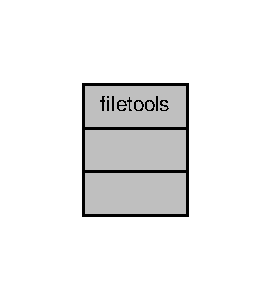
\includegraphics[width=130pt]{classfiletools__coll__graph}
\end{center}
\end{figure}
\subsection*{Data Types}
\begin{DoxyCompactItemize}
\item 
interface \hyperlink{interfacefiletools_1_1c_find_entry}{c\-Find\-Entry}
\item 
interface \hyperlink{interfacefiletools_1_1c_matrix_read}{c\-Matrix\-Read}
\item 
interface \hyperlink{interfacefiletools_1_1d_find_entry}{d\-Find\-Entry}
\item 
interface \hyperlink{interfacefiletools_1_1d_matrix_read}{d\-Matrix\-Read}
\item 
interface \hyperlink{interfacefiletools_1_1find_entry}{find\-Entry}
\item 
interface \hyperlink{interfacefiletools_1_1h_count}{h\-Count}
\item 
interface \hyperlink{interfacefiletools_1_1i_find_entry}{i\-Find\-Entry}
\item 
interface \hyperlink{interfacefiletools_1_1i_matrix_read}{i\-Matrix\-Read}
\item 
interface \hyperlink{interfacefiletools_1_1matrix_read}{matrix\-Read}
\item 
interface \hyperlink{interfacefiletools_1_1read_keyword}{read\-Keyword}
\item 
interface \hyperlink{interfacefiletools_1_1rew_unit}{rew\-Unit}
\item 
interface \hyperlink{interfacefiletools_1_1v_count}{v\-Count}
\end{DoxyCompactItemize}


\subsection{Detailed Description}
This module collects all the interfaces of the procedures useful to read data from files. \begin{DoxyAuthor}{Author}
Andrea Facci. 
\end{DoxyAuthor}


Definition at line 39 of file file\-Tools.\-f90.



The documentation for this module was generated from the following file\-:\begin{DoxyCompactItemize}
\item 
/home/\-Progetti/\-Siat/\-Ottimizzatore/src/\hyperlink{file_tools_8f90}{file\-Tools.\-f90}\end{DoxyCompactItemize}

\hypertarget{interfacefiletools_1_1find_entry}{\section{filetools\-:\-:find\-Entry Interface Reference}
\label{interfacefiletools_1_1find_entry}\index{filetools\-::find\-Entry@{filetools\-::find\-Entry}}
}


Collaboration diagram for filetools\-:\-:find\-Entry\-:\nopagebreak
\begin{figure}[H]
\begin{center}
\leavevmode
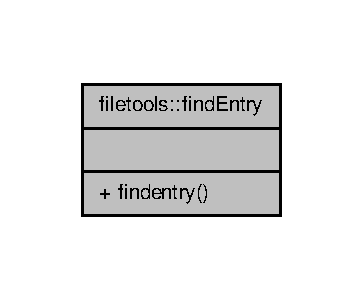
\includegraphics[width=174pt]{interfacefiletools_1_1find_entry__coll__graph}
\end{center}
\end{figure}
\subsection*{Public Member Functions}
\begin{DoxyCompactItemize}
\item 
subroutine \hyperlink{interfacefiletools_1_1find_entry_a850f330e19410327017ded432bedab00}{findentry} (entry, the\-Unit, rew, valore, is\-Present, n\-Row)
\end{DoxyCompactItemize}


\subsection{Detailed Description}


Definition at line 153 of file file\-Tools.\-f90.



\subsection{Member Function/\-Subroutine Documentation}
\hypertarget{interfacefiletools_1_1find_entry_a850f330e19410327017ded432bedab00}{\index{filetools\-::find\-Entry@{filetools\-::find\-Entry}!findentry@{findentry}}
\index{findentry@{findentry}!filetools::findEntry@{filetools\-::find\-Entry}}
\subsubsection[{findentry}]{\setlength{\rightskip}{0pt plus 5cm}subroutine filetools\-::find\-Entry\-::findentry (
\begin{DoxyParamCaption}
\item[{character(len=$\ast$), intent(in)}]{entry, }
\item[{integer, intent(in)}]{the\-Unit, }
\item[{logical, intent(in), optional}]{rew, }
\item[{character(len=100), intent(out), optional}]{valore, }
\item[{logical, intent(out), optional}]{is\-Present, }
\item[{integer, intent(out), optional}]{n\-Row}
\end{DoxyParamCaption}
)}}\label{interfacefiletools_1_1find_entry_a850f330e19410327017ded432bedab00}


Definition at line 153 of file file\-Tools.\-f90.



The documentation for this interface was generated from the following file\-:\begin{DoxyCompactItemize}
\item 
/home/\-Progetti/\-Siat/\-Ottimizzatore/src/\hyperlink{file_tools_8f90}{file\-Tools.\-f90}\end{DoxyCompactItemize}

\hypertarget{classgraphtools}{\section{graphtools Module Reference}
\label{classgraphtools}\index{graphtools@{graphtools}}
}


Collaboration diagram for graphtools\-:
\nopagebreak
\begin{figure}[H]
\begin{center}
\leavevmode
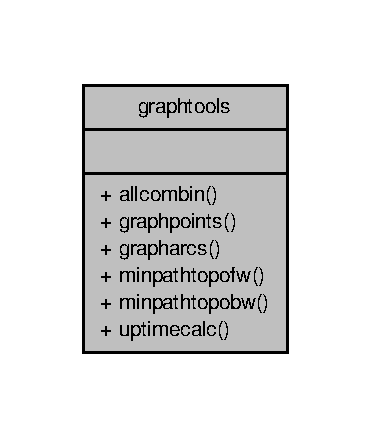
\includegraphics[width=178pt]{classgraphtools__coll__graph}
\end{center}
\end{figure}
\subsection*{Data Types}
\begin{DoxyCompactItemize}
\item 
interface \hyperlink{interfacegraphtools_1_1constraints}{constraints}
\item 
interface \hyperlink{interfacegraphtools_1_1obj_function}{obj\-Function}
\item 
interface \hyperlink{interfacegraphtools_1_1time_constr}{time\-Constr}
\end{DoxyCompactItemize}
\subsection*{Public Member Functions}
\begin{DoxyCompactItemize}
\item 
subroutine \hyperlink{classgraphtools_a4607d975b5dd57d2ca7fcdbab2b1ef56}{allcombin} (icm, dcm, imax, m, targ)
\begin{DoxyCompactList}\small\item\em Generates all the combinations of the set points, staring from the set-\/point vectors that are stored in the columns of \char`\"{}cm\char`\"{}. \end{DoxyCompactList}\item 
subroutine \hyperlink{classgraphtools_a94b8e6e5a3d3cc0c3bedbe00d57fc2f9}{graphpoints}
\begin{DoxyCompactList}\small\item\em Generates the graph veteces, starting from the array of the set-\/point combinations. \end{DoxyCompactList}\item 
subroutine \hyperlink{classgraphtools_a47c76f30f7f4917536f94c642ffca865}{grapharcs}
\begin{DoxyCompactList}\small\item\em Generates the grapsh arcs. \end{DoxyCompactList}\item 
subroutine \hyperlink{classgraphtools_ade3577b19aec190e8e056f041bc8afdf}{minpathtopofw} (ott\-Load, min\-Cost)
\begin{DoxyCompactList}\small\item\em Miniumum path detemination. \end{DoxyCompactList}\item 
subroutine \hyperlink{classgraphtools_abef4e47145f628bc6d3001d4f6bd9601}{minpathtopobw} (ott\-Load, min\-Cost, up\-Time, min\-Path)
\begin{DoxyCompactList}\small\item\em Miniumum path detemination. \end{DoxyCompactList}\item 
real(kind(1.d0)) function, \\*
dimension(2 $\ast$nm) \hyperlink{classgraphtools_ac61c9cdfdbeb51411798714a7ba88c3e}{uptimecalc} (up\-T, c, t)
\end{DoxyCompactItemize}


\subsection{Detailed Description}


Definition at line 34 of file graph\-Tools.\-f90.



\subsection{Member Function/\-Subroutine Documentation}
\hypertarget{classgraphtools_a4607d975b5dd57d2ca7fcdbab2b1ef56}{\index{graphtools@{graphtools}!allcombin@{allcombin}}
\index{allcombin@{allcombin}!graphtools@{graphtools}}
\subsubsection[{allcombin}]{\setlength{\rightskip}{0pt plus 5cm}subroutine graphtools\-::allcombin (
\begin{DoxyParamCaption}
\item[{integer, dimension(maxval(imax),m), intent(in), optional}]{icm, }
\item[{real(kind(1.d0)), dimension(maxval(imax),m), intent(in), optional}]{dcm, }
\item[{integer, dimension(m), intent(in)}]{imax, }
\item[{integer, intent(in)}]{m, }
\item[{character(len=100), intent(in), optional}]{targ}
\end{DoxyParamCaption}
)}}\label{classgraphtools_a4607d975b5dd57d2ca7fcdbab2b1ef56}
Generates all the combinations of the set points, staring from the set-\/point vectors that are stored in the columns of \char`\"{}cm\char`\"{}. Each row of the array \char`\"{}comb\char`\"{} represents a set-\/point of the plant. The total number of states of the plant is also returned in the variable \char`\"{}n\-Comb\char`\"{} \begin{DoxyAuthor}{Author}
Andrea Facci 
\end{DoxyAuthor}


Definition at line 97 of file graph\-Tools.\-f90.



References abortexecution().



Referenced by main().

\hypertarget{classgraphtools_a47c76f30f7f4917536f94c642ffca865}{\index{graphtools@{graphtools}!grapharcs@{grapharcs}}
\index{grapharcs@{grapharcs}!graphtools@{graphtools}}
\subsubsection[{grapharcs}]{\setlength{\rightskip}{0pt plus 5cm}subroutine graphtools\-::grapharcs (
\begin{DoxyParamCaption}
{}
\end{DoxyParamCaption}
)}}\label{classgraphtools_a47c76f30f7f4917536f94c642ffca865}
Generates the grapsh arcs. Note that only vertex relative to consecutive time-\/steps are connected and that arcs are oriented in the direction of increasing time. Arcs are stored in the form of a predecessor list \char`\"{}pred\-List\char`\"{}, that associates to each node all its predecessors. A weight is assiciated to each element of the predecessor list, equal to the weight of the predecessor vertex plus a cost connected to the variation of state between the actual and predecessor state. \[ arcCost(i,j) = pointCost(c(i)) + fireCost(i,j) \] The number of predecessors for each vertex is asle stored in the \char`\"{}n\-Pre(i)\char`\"{} array. 

Definition at line 290 of file graph\-Tools.\-f90.



References economy\-::firecost(), and myarithmetic\-::rnan().



Referenced by main().

\hypertarget{classgraphtools_a94b8e6e5a3d3cc0c3bedbe00d57fc2f9}{\index{graphtools@{graphtools}!graphpoints@{graphpoints}}
\index{graphpoints@{graphpoints}!graphtools@{graphtools}}
\subsubsection[{graphpoints}]{\setlength{\rightskip}{0pt plus 5cm}subroutine graphtools\-::graphpoints (
\begin{DoxyParamCaption}
{}
\end{DoxyParamCaption}
)}}\label{classgraphtools_a94b8e6e5a3d3cc0c3bedbe00d57fc2f9}
Generates the graph veteces, starting from the array of the set-\/point combinations. For each time-\/step determines which plant state respects the energy (staitc) constraints, and associates them to a graph vertex. A weight, that accounts for the costs/revenues of operating the power plant from time-\/step t to t+1 at the vertex state, is also calculated for each vertex. The time-\/step relative to each vertex and the number of verteces for each time step are associated to \char`\"{}point\-Time\char`\"{} and \char`\"{}nt\char`\"{} vectors respectively. Vertex 0 will be the starting point of the graph and vertex n\-Point + 1 the arriving point \begin{DoxyAuthor}{Author}
Andrea Facci. 
\end{DoxyAuthor}


Definition at line 199 of file graph\-Tools.\-f90.



References abortexecution(), mathtools\-::locaterow(), and objfunction().



Referenced by main().

\hypertarget{classgraphtools_abef4e47145f628bc6d3001d4f6bd9601}{\index{graphtools@{graphtools}!minpathtopobw@{minpathtopobw}}
\index{minpathtopobw@{minpathtopobw}!graphtools@{graphtools}}
\subsubsection[{minpathtopobw}]{\setlength{\rightskip}{0pt plus 5cm}subroutine graphtools\-::minpathtopobw (
\begin{DoxyParamCaption}
\item[{integer, dimension(0\-:ntime+1,nm), intent(out)}]{ott\-Load, }
\item[{real(kind(1.d0)), intent(out)}]{min\-Cost, }
\item[{real(kind(1.d0)), dimension(0\-:ntime+1,2$\ast$nm), intent(out)}]{up\-Time, }
\item[{integer, dimension(0\-:ntime+1)}]{min\-Path}
\end{DoxyParamCaption}
)}}\label{classgraphtools_abef4e47145f628bc6d3001d4f6bd9601}
This function determies the minumum path that connects the start point (0) to the arrival point of the graph (n\-Point + 1), using dynamic programming. Specifically the oprimizazion the algorithm is tailored to sort acyclic graphs with topolgical ordering. \begin{DoxyAuthor}{Author}
Andrea Facci. 
\end{DoxyAuthor}


Definition at line 452 of file graph\-Tools.\-f90.



References mathtools\-::locaterow(), timeconstr(), and uptimecalc().



Referenced by main().

\hypertarget{classgraphtools_ade3577b19aec190e8e056f041bc8afdf}{\index{graphtools@{graphtools}!minpathtopofw@{minpathtopofw}}
\index{minpathtopofw@{minpathtopofw}!graphtools@{graphtools}}
\subsubsection[{minpathtopofw}]{\setlength{\rightskip}{0pt plus 5cm}subroutine graphtools\-::minpathtopofw (
\begin{DoxyParamCaption}
\item[{integer, dimension(0\-:ntime+1,nm), intent(out)}]{ott\-Load, }
\item[{real(kind(1.d0)), intent(out)}]{min\-Cost}
\end{DoxyParamCaption}
)}}\label{classgraphtools_ade3577b19aec190e8e056f041bc8afdf}
This function determies the minumum path that connects the start point (0) to the arrival point of the graph (n\-Point + 1), using dynamic programming. Specifically the oprimizazion the algorithm is tailored to sort acyclic graphs with topolgical ordering. \begin{DoxyAuthor}{Author}
Andrea Facci. 
\end{DoxyAuthor}


Definition at line 394 of file graph\-Tools.\-f90.



Referenced by main().

\hypertarget{classgraphtools_ac61c9cdfdbeb51411798714a7ba88c3e}{\index{graphtools@{graphtools}!uptimecalc@{uptimecalc}}
\index{uptimecalc@{uptimecalc}!graphtools@{graphtools}}
\subsubsection[{uptimecalc}]{\setlength{\rightskip}{0pt plus 5cm}real(kind(1.d0)) function, dimension(2$\ast$nm) graphtools\-::uptimecalc (
\begin{DoxyParamCaption}
\item[{real(kind(1.d0)), dimension(2$\ast$nm)}]{up\-T, }
\item[{integer, dimension(nm), intent(in)}]{c, }
\item[{integer, intent(in)}]{t}
\end{DoxyParamCaption}
)}}\label{classgraphtools_ac61c9cdfdbeb51411798714a7ba88c3e}


Definition at line 529 of file graph\-Tools.\-f90.



Referenced by minpathtopobw().



The documentation for this module was generated from the following file\-:\begin{DoxyCompactItemize}
\item 
/home/andrea/\-Desktop/\-Fortran\-Code\-B\-W/src/\hyperlink{graph_tools_8f90}{graph\-Tools.\-f90}\end{DoxyCompactItemize}

\hypertarget{interfacefiletools_1_1h_count}{\section{filetools\-:\-:h\-Count Interface Reference}
\label{interfacefiletools_1_1h_count}\index{filetools\-::h\-Count@{filetools\-::h\-Count}}
}


Collaboration diagram for filetools\-:\-:h\-Count\-:\nopagebreak
\begin{figure}[H]
\begin{center}
\leavevmode
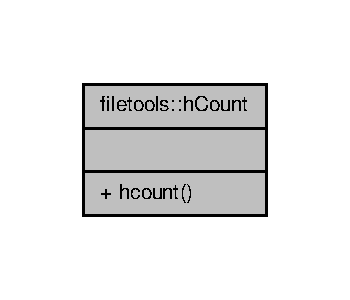
\includegraphics[width=168pt]{interfacefiletools_1_1h_count__coll__graph}
\end{center}
\end{figure}
\subsection*{Public Member Functions}
\begin{DoxyCompactItemize}
\item 
integer function \hyperlink{interfacefiletools_1_1h_count_afb6ca416dfce200b6ce23667f215771c}{hcount} (value\-\_\-, first\-\_\-, last\-\_\-)
\end{DoxyCompactItemize}


\subsection{Detailed Description}


Definition at line 58 of file file\-Tools.\-f90.



\subsection{Member Function/\-Subroutine Documentation}
\hypertarget{interfacefiletools_1_1h_count_afb6ca416dfce200b6ce23667f215771c}{\index{filetools\-::h\-Count@{filetools\-::h\-Count}!hcount@{hcount}}
\index{hcount@{hcount}!filetools::hCount@{filetools\-::h\-Count}}
\subsubsection[{hcount}]{\setlength{\rightskip}{0pt plus 5cm}integer function filetools\-::h\-Count\-::hcount (
\begin{DoxyParamCaption}
\item[{character(len=100), intent(in)}]{value\-\_\-, }
\item[{character(len=1), optional}]{first\-\_\-, }
\item[{character(len=1), optional}]{last\-\_\-}
\end{DoxyParamCaption}
)}}\label{interfacefiletools_1_1h_count_afb6ca416dfce200b6ce23667f215771c}


Definition at line 58 of file file\-Tools.\-f90.



The documentation for this interface was generated from the following file\-:\begin{DoxyCompactItemize}
\item 
/home/andrea/\-Desktop/\-Fortran\-Code\-B\-W/src/\hyperlink{file_tools_8f90}{file\-Tools.\-f90}\end{DoxyCompactItemize}

\hypertarget{interfacefiletools_1_1i_find_entry}{\section{filetools\-:\-:i\-Find\-Entry Interface Reference}
\label{interfacefiletools_1_1i_find_entry}\index{filetools\-::i\-Find\-Entry@{filetools\-::i\-Find\-Entry}}
}


Collaboration diagram for filetools\-:\-:i\-Find\-Entry\-:\nopagebreak
\begin{figure}[H]
\begin{center}
\leavevmode
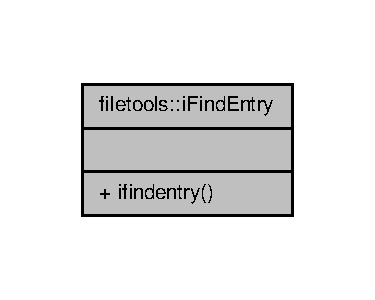
\includegraphics[width=180pt]{interfacefiletools_1_1i_find_entry__coll__graph}
\end{center}
\end{figure}
\subsection*{Public Member Functions}
\begin{DoxyCompactItemize}
\item 
subroutine \hyperlink{interfacefiletools_1_1i_find_entry_acc5d0e736fc0e81737c4ae294410f3c8}{ifindentry} (entry, n, the\-Unit, rew, valore, is\-Present, n\-Row)
\end{DoxyCompactItemize}


\subsection{Detailed Description}


Definition at line 102 of file file\-Tools.\-f90.



\subsection{Member Function/\-Subroutine Documentation}
\hypertarget{interfacefiletools_1_1i_find_entry_acc5d0e736fc0e81737c4ae294410f3c8}{\index{filetools\-::i\-Find\-Entry@{filetools\-::i\-Find\-Entry}!ifindentry@{ifindentry}}
\index{ifindentry@{ifindentry}!filetools::iFindEntry@{filetools\-::i\-Find\-Entry}}
\subsubsection[{ifindentry}]{\setlength{\rightskip}{0pt plus 5cm}subroutine filetools\-::i\-Find\-Entry\-::ifindentry (
\begin{DoxyParamCaption}
\item[{character(len=100), intent(in)}]{entry, }
\item[{integer, intent(in)}]{n, }
\item[{integer, intent(in)}]{the\-Unit, }
\item[{logical, intent(in), optional}]{rew, }
\item[{integer, dimension(n), intent(out), optional}]{valore, }
\item[{logical, intent(out), optional}]{is\-Present, }
\item[{integer, intent(out), optional}]{n\-Row}
\end{DoxyParamCaption}
)}}\label{interfacefiletools_1_1i_find_entry_acc5d0e736fc0e81737c4ae294410f3c8}


Definition at line 102 of file file\-Tools.\-f90.



The documentation for this interface was generated from the following file\-:\begin{DoxyCompactItemize}
\item 
/home/andrea/\-Desktop/\-Fortran\-Code\-B\-W/src/\hyperlink{file_tools_8f90}{file\-Tools.\-f90}\end{DoxyCompactItemize}

\hypertarget{interfacefiletools_1_1i_matrix_read}{\section{filetools\-:\-:i\-Matrix\-Read Interface Reference}
\label{interfacefiletools_1_1i_matrix_read}\index{filetools\-::i\-Matrix\-Read@{filetools\-::i\-Matrix\-Read}}
}


Collaboration diagram for filetools\-:\-:i\-Matrix\-Read\-:\nopagebreak
\begin{figure}[H]
\begin{center}
\leavevmode
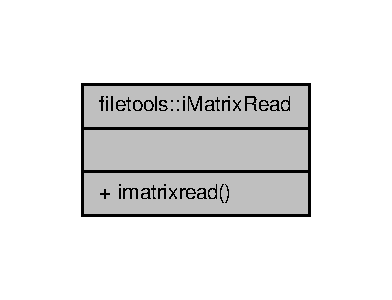
\includegraphics[width=188pt]{interfacefiletools_1_1i_matrix_read__coll__graph}
\end{center}
\end{figure}
\subsection*{Public Member Functions}
\begin{DoxyCompactItemize}
\item 
real(kind=prec) function, \\*
dimension(nline, ncol) \hyperlink{interfacefiletools_1_1i_matrix_read_afa8b378d4dfdc6516ef2c90a9d9d89ca}{imatrixread} (the\-Unit, nline, ncol, first\-\_\-, last\-\_\-)
\end{DoxyCompactItemize}


\subsection{Detailed Description}


Definition at line 81 of file file\-Tools.\-f90.



\subsection{Member Function/\-Subroutine Documentation}
\hypertarget{interfacefiletools_1_1i_matrix_read_afa8b378d4dfdc6516ef2c90a9d9d89ca}{\index{filetools\-::i\-Matrix\-Read@{filetools\-::i\-Matrix\-Read}!imatrixread@{imatrixread}}
\index{imatrixread@{imatrixread}!filetools::iMatrixRead@{filetools\-::i\-Matrix\-Read}}
\subsubsection[{imatrixread}]{\setlength{\rightskip}{0pt plus 5cm}real(kind = prec) function, dimension(nline,ncol) filetools\-::i\-Matrix\-Read\-::imatrixread (
\begin{DoxyParamCaption}
\item[{integer, intent(in)}]{the\-Unit, }
\item[{integer, intent(in)}]{nline, }
\item[{integer, intent(in)}]{ncol, }
\item[{character(len=1), optional}]{first\-\_\-, }
\item[{character(len=1), optional}]{last\-\_\-}
\end{DoxyParamCaption}
)}}\label{interfacefiletools_1_1i_matrix_read_afa8b378d4dfdc6516ef2c90a9d9d89ca}


Definition at line 81 of file file\-Tools.\-f90.



The documentation for this interface was generated from the following file\-:\begin{DoxyCompactItemize}
\item 
/home/\-Progetti/\-Siat/\-Ottimizzatore/src/\hyperlink{file_tools_8f90}{file\-Tools.\-f90}\end{DoxyCompactItemize}

\hypertarget{classinputvar}{\section{inputvar Module Reference}
\label{classinputvar}\index{inputvar@{inputvar}}
}


Input variables collection.  




Collaboration diagram for inputvar\-:\nopagebreak
\begin{figure}[H]
\begin{center}
\leavevmode
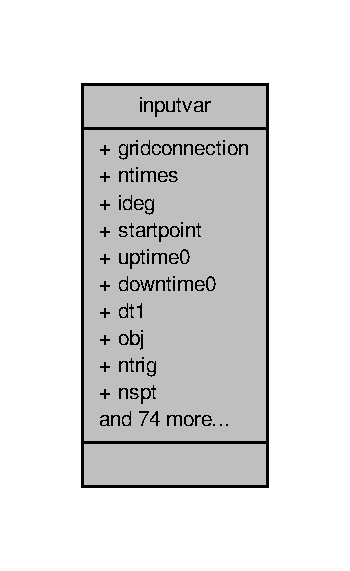
\includegraphics[width=168pt]{classinputvar__coll__graph}
\end{center}
\end{figure}
\subsection*{Public Attributes}
\begin{DoxyCompactItemize}
\item 
logical, dimension(3) \hyperlink{classinputvar_a4bacf572842e302cf317a3cc5e95a9b9}{iprio} = .false.
\item 
character(len=20) \hyperlink{classinputvar_a8488f705094b7c59cf8cb06939fe9a7a}{gridconnection}
\item 
integer \hyperlink{classinputvar_a98d384e0347fb055110c18572dbdb522}{ntimes}
\item 
logical \hyperlink{classinputvar_a62235e6c8b16a98c1aea10ac01e11ac9}{ideg}
\item 
real(kind=prec), dimension(\-:), \\*
allocatable \hyperlink{classinputvar_a3b9acf8a358a0bad89d622cbbbab638f}{startpoint}
\item 
real(kind=prec), dimension(\-:), \\*
allocatable \hyperlink{classinputvar_a3938be0ea72158eee837e2a8c08f29e0}{uptime0}
\item 
real(kind=prec), dimension(\-:), \\*
allocatable \hyperlink{classinputvar_aaab84ab253f188eacce25a200a4ab300}{downtime0}
\item 
real(kind=prec) \hyperlink{classinputvar_a62c9f9492040ef5e03091380533f2c0f}{dt1}
\item 
real(kind=prec) \hyperlink{classinputvar_ad02af5c5e2d12134398545c12e832b9b}{k\-\_\-tr}
\item 
real(kind=prec) \hyperlink{classinputvar_a021273f9a287d8d4c9fcd0651bf17d8e}{k\-\_\-el}
\item 
real(kind=prec) \hyperlink{classinputvar_a52f3b90c5f4c7bb282ebc24e762032a2}{c\-\_\-tr}
\item 
real(kind=prec) \hyperlink{classinputvar_afe1c70c120d3938f07fa818f015ad52d}{c\-\_\-st}
\item 
real(kind=prec) \hyperlink{classinputvar_aeb238280e9c8d1526ff6c11142a32cda}{pefgrid}
\item 
real(kind=prec) \hyperlink{classinputvar_a5f5ab91e72a9ea0ec51d7f621d01108b}{isocth}
\item 
real(kind=prec) \hyperlink{classinputvar_a144453fc737cf5fa64bf329abb73d1c6}{esocth}
\item 
real(kind=prec) \hyperlink{classinputvar_a398c551573b9e71aaae3ba84991c6b81}{isocel}
\item 
real(kind=prec) \hyperlink{classinputvar_a761214782c22ee31b6da74c0984cb9e2}{esocel}
\item 
character(len=100) \hyperlink{classinputvar_ab5d2f467a214e31204c18a24582b81bb}{obj}
\item 
character(len=100) \hyperlink{classinputvar_ad9c1a09ed4bd46ad673997ee302451a4}{method}
\item 
character(len=100) \hyperlink{classinputvar_a6e328846c755855ac2ac87d5a63d402a}{strategy}
\item 
logical \hyperlink{classinputvar_ae3e0dfd2907bb36d0f62715b24f63536}{writepower} = .false.
\item 
logical \hyperlink{classinputvar_ae3e52c17a47fe8dd3e860abff881cfb0}{writeenergy} = .false.
\item 
logical \hyperlink{classinputvar_a7d67f2fa2027e1d60264f442eef9759c}{writeefficiency} = .false.
\item 
logical \hyperlink{classinputvar_afd3b4bc26c396eaba06cecc08717acf1}{writeelectricrev} = .false.
\item 
logical \hyperlink{classinputvar_ae7817d3a1abb7e02fdd1d3f40b45a4e8}{writethermalrev} = .false.
\item 
logical \hyperlink{classinputvar_a2d475a99a1a0efcca534104cf8e2efb5}{writechillingrev} = .false.
\item 
logical \hyperlink{classinputvar_ad6cafaf46b6d0f5bfaeb1ca26ccd0c68}{writedemand} = .false.
\item 
logical \hyperlink{classinputvar_a97c8b194b0db24c1c790d57bcc7b0f70}{writeinput} = .false.
\item 
logical \hyperlink{classinputvar_a5fa854d48ca73d10b807273f373076b2}{writecosts} = .false.
\item 
logical \hyperlink{classinputvar_a676701049b4d18d378d94894b1fcae7b}{writetrig} = .false.
\item 
logical \hyperlink{classinputvar_adfc2c014d1631c831bd700d9ff13dcff}{writeboi} = .false.
\item 
logical \hyperlink{classinputvar_a6e34f329672526cc9e682125013ce5e7}{writechi} = .false.
\item 
logical \hyperlink{classinputvar_a81f46f9ef3ef3bdb78c79994791f3472}{writepec} = .false.
\item 
logical \hyperlink{classinputvar_aaea9119ed7c4fbad274831007b696f46}{writeren} = .false.
\item 
logical \hyperlink{classinputvar_aa558f36057a5ae647fb16b9659b90d04}{global} = .false.
\item 
logical \hyperlink{classinputvar_a04f11d38b133803024202cc546abddc3}{useeuristics} = .false.
\item 
logical, dimension(5) \hyperlink{classinputvar_a17bd2d4ef6c3b43e7b2d447f1fab021e}{kpec} = .false.
\item 
logical \hyperlink{classinputvar_af90e08308cf6a7de1480cfde429187d3}{ipec} = .false.
\item 
integer \hyperlink{classinputvar_ae4403f5c5b16bf2cbd2b607a87e5ee9a}{ntrig}
\item 
integer, dimension(\-:), allocatable \hyperlink{classinputvar_a0c86e9a7915872ee547e5bd8802611e7}{nspt}
\item 
integer, dimension(\-:), allocatable \hyperlink{classinputvar_a2bfcb389a7fba156b8c1146150a71f51}{netaelt}
\item 
integer, dimension(\-:), allocatable \hyperlink{classinputvar_acebcf3d64f116183dd364e920288729f}{netatht}
\item 
integer, dimension(\-:), allocatable \hyperlink{classinputvar_a7f82eda09f512dfe2f28f82efc5187ad}{netacht}
\item 
integer, dimension(\-:), allocatable \hyperlink{classinputvar_ad5c9bbca95851da9fa84642ea414e6be}{ntct}
\item 
integer, dimension(\-:), allocatable \hyperlink{classinputvar_a0f5eeaa6713564c7a3aa547b8ce8bae9}{npct}
\item 
integer, dimension(\-:), allocatable \hyperlink{classinputvar_aecb7a7ef500aee2174166b23b5c72e2a}{nact}
\item 
integer, dimension(\-:), allocatable \hyperlink{classinputvar_aa06cb5d284b385bcfed4e6f34efa534f}{trigpriority}
\item 
real(kind=prec), dimension(\-:), \\*
allocatable \hyperlink{classinputvar_a0a9434332c855a12ef886b675af68d35}{pmaxt}
\item 
real(kind=prec), dimension(\-:), \\*
allocatable \hyperlink{classinputvar_a85ccff6d868e650d2255bb9faa7c31be}{fuelcostt}
\item 
real(kind=prec), dimension(\-:), \\*
allocatable \hyperlink{classinputvar_afe467edd87c4c589d3ad9d5b14825f94}{fuellhvt}
\item 
real(kind=prec), dimension(\-:), \\*
allocatable \hyperlink{classinputvar_a04abed47801bdfcda1ecba21b90ab85b}{lifet}
\item 
real(kind=prec), dimension(\-:), \\*
allocatable \hyperlink{classinputvar_ab6d8921a6209783f0f51673c842f94b5}{peft}
\item 
real(kind=prec), dimension(\-:), \\*
allocatable \hyperlink{classinputvar_a1f575248c5370894cd5abbad18ace926}{pecont}
\item 
real(kind=prec), dimension(\-:), \\*
allocatable \hyperlink{classinputvar_a57526f25accbe0af7902997bd9cde614}{firecostt}
\item 
real(kind=prec), dimension(\-:), \\*
allocatable \hyperlink{classinputvar_abeac95d7e558ca06d4456187b380fdbc}{maintcostt}
\item 
real(kind=prec), dimension(\-:), \\*
allocatable \hyperlink{classinputvar_a90d0b599ed6468fc322cf2fbd6b4ec95}{minuptimet}
\item 
real(kind=prec), dimension(\-:), \\*
allocatable \hyperlink{classinputvar_aca351a4427897a65d991d46243fadc34}{mindowntimet}
\item 
real(kind=prec), dimension(\-:,\-:), \\*
allocatable \hyperlink{classinputvar_aa1da1474767137ee483ef4253b7cef85}{spt}
\item 
real(kind=prec), dimension(\-:,\-:,\-:), \\*
allocatable \hyperlink{classinputvar_af7479b2afabbd7d596d91bb1319b0a8e}{etaelt}
\item 
real(kind=prec), dimension(\-:,\-:,\-:), \\*
allocatable \hyperlink{classinputvar_a93c858e92300ce7dfc06627cbc72d681}{etatht}
\item 
real(kind=prec), dimension(\-:,\-:,\-:), \\*
allocatable \hyperlink{classinputvar_a7cd43a0a5d5ddb8d50af96d4c4f81bea}{etacht}
\item 
real(kind=prec), dimension(\-:,\-:,\-:), \\*
allocatable \hyperlink{classinputvar_a918356589b5f04f76333e6a65de35fb8}{tempcorrt}
\item 
real(kind=prec), dimension(\-:,\-:,\-:), \\*
allocatable \hyperlink{classinputvar_a4dc6d715b00d35dbff920be5c37c1d89}{prescorrt}
\item 
real(kind=prec), dimension(\-:,\-:,\-:), \\*
allocatable \hyperlink{classinputvar_a1405821026cba8a541725451f5a6f8dd}{altcorrt}
\item 
character(len=50), dimension(\-:), \\*
allocatable \hyperlink{classinputvar_afb7d5163d753c7bbd2c1505e8ee68197}{tect}
\item 
integer \hyperlink{classinputvar_a168bc1dcb73e68b3620991b6494f3797}{nboi}
\item 
integer, dimension(\-:), allocatable \hyperlink{classinputvar_aa1e78ecd4b3cbb3f08b770cf604a5d3d}{nspb}
\item 
integer, dimension(\-:), allocatable \hyperlink{classinputvar_af109996c7b379bac5d6c3d89c5b6df1d}{netab}
\item 
integer, dimension(\-:), allocatable \hyperlink{classinputvar_a41aaaf97cb1f1e815c73bcfa5f975be3}{ntcb}
\item 
integer, dimension(\-:), allocatable \hyperlink{classinputvar_a4f83c89634ccb8f94fca08a023648791}{npcb}
\item 
integer, dimension(\-:), allocatable \hyperlink{classinputvar_ae517f545e388b4352b7941203efa8449}{nacb}
\item 
integer, dimension(\-:), allocatable \hyperlink{classinputvar_a87efe639d66848f1a52e1c265e175e2c}{boipriority}
\item 
real(kind=prec), dimension(\-:), \\*
allocatable \hyperlink{classinputvar_a29e37a8460969d1438ed9aeb5d37d798}{pmaxb}
\item 
real(kind=prec), dimension(\-:), \\*
allocatable \hyperlink{classinputvar_a7ba5eba73efe4e693920d6af7782e58e}{fuelcostb}
\item 
real(kind=prec), dimension(\-:), \\*
allocatable \hyperlink{classinputvar_a3cd62c9288fded8bd8de8066cbb3ca20}{fuellhvb}
\item 
real(kind=prec), dimension(\-:), \\*
allocatable \hyperlink{classinputvar_a3484e64c94e8f61527a9843039243703}{pefb}
\item 
real(kind=prec), dimension(\-:), \\*
allocatable \hyperlink{classinputvar_adfc7efd23b85b75ea9411b9da5e8ccbd}{peconb}
\item 
real(kind=prec), dimension(\-:), \\*
allocatable \hyperlink{classinputvar_a74dcd10e62524e2f5145df13548eae82}{lifeb}
\item 
real(kind=prec), dimension(\-:), \\*
allocatable \hyperlink{classinputvar_a1560f8312d0c0606566ee8f7e21c1e49}{firecostb}
\item 
real(kind=prec), dimension(\-:), \\*
allocatable \hyperlink{classinputvar_ac52f743f02f10e96c455d94c3cdc0fe8}{maintcostb}
\item 
real(kind=prec), dimension(\-:), \\*
allocatable \hyperlink{classinputvar_a699644b9b98282661cd55dc10d96dbcb}{minuptimeb}
\item 
real(kind=prec), dimension(\-:), \\*
allocatable \hyperlink{classinputvar_ae93da8603e9899963da53596705b1d98}{mindowntimeb}
\item 
real(kind=prec), dimension(\-:,\-:), \\*
allocatable \hyperlink{classinputvar_acd5ae0efcfc5e54e9c73d085132bcf5a}{spb}
\item 
real(kind=prec), dimension(\-:,\-:,\-:), \\*
allocatable \hyperlink{classinputvar_adba062c6d3ce600124e2cd8943f7c6e6}{etab}
\item 
real(kind=prec), dimension(\-:,\-:,\-:), \\*
allocatable \hyperlink{classinputvar_a4270f23d875d4a85d7bd5d6699205d03}{tempcorrb}
\item 
real(kind=prec), dimension(\-:,\-:,\-:), \\*
allocatable \hyperlink{classinputvar_a4de979203fa5e65fe0cbfd77c60654ae}{prescorrb}
\item 
real(kind=prec), dimension(\-:,\-:,\-:), \\*
allocatable \hyperlink{classinputvar_a3fb49f59a3c5a2a19350be6bea0d69c2}{altcorrb}
\item 
character(len=50), dimension(\-:), \\*
allocatable \hyperlink{classinputvar_ab2486a625a1ff1aaf70cb9e38d8c07db}{tecb}
\item 
integer \hyperlink{classinputvar_ac34eff504af528e971c7174dfcb39028}{nchi}
\item 
integer, dimension(\-:), allocatable \hyperlink{classinputvar_aad6ce13b0378ba79e193cb3738e2d938}{nspc}
\item 
integer, dimension(\-:), allocatable \hyperlink{classinputvar_af28da5ec88564638bee476f2a37f5308}{nsizec}
\item 
integer, dimension(\-:), allocatable \hyperlink{classinputvar_ad9998f4f97f100bf6294fb8fa083bfe7}{netac}
\item 
integer, dimension(\-:), allocatable \hyperlink{classinputvar_aaf3cc67ce289abacf61f20f5fdcfc3f6}{ntcc}
\item 
integer, dimension(\-:), allocatable \hyperlink{classinputvar_a78f4d80d45d564c96dd9101258656f66}{npcc}
\item 
integer, dimension(\-:), allocatable \hyperlink{classinputvar_a8e4bb497a3825e6f554e3268dd2bbd63}{nacc}
\item 
integer, dimension(\-:), allocatable \hyperlink{classinputvar_a2cb9252c074d0ed99a8ec738dfc04ee2}{chipriority}
\item 
real(kind=prec), dimension(\-:), \\*
allocatable \hyperlink{classinputvar_a93b555571bee30038d48c86de7ab5c14}{pmaxc}
\item 
real(kind=prec), dimension(\-:), \\*
allocatable \hyperlink{classinputvar_afa2d0c05087f3cda5d3e984037a2a354}{firecostc}
\item 
real(kind=prec), dimension(\-:), \\*
allocatable \hyperlink{classinputvar_a4371de15edf20ae9883b07b3b843655d}{maintcostc}
\item 
real(kind=prec), dimension(\-:), \\*
allocatable \hyperlink{classinputvar_a1c2a4cc32567b94cb7a884d3731bb5f4}{minuptimec}
\item 
real(kind=prec), dimension(\-:), \\*
allocatable \hyperlink{classinputvar_a9bb1424e04e5c89d561d2316045f98d4}{mindowntimec}
\item 
real(kind=prec), dimension(\-:,\-:), \\*
allocatable \hyperlink{classinputvar_a7a6b03a57941065017f0fe71a9d641f1}{spc}
\item 
real(kind=prec), dimension(\-:,\-:,\-:), \\*
allocatable \hyperlink{classinputvar_a3c6d7517ec3f9097a8d4264b50e61b48}{etac}
\item 
real(kind=prec), dimension(\-:,\-:,\-:), \\*
allocatable \hyperlink{classinputvar_a378a362979a22545cd843bbf687ca511}{tempcorrc}
\item 
real(kind=prec), dimension(\-:,\-:,\-:), \\*
allocatable \hyperlink{classinputvar_a4ad15e4562f67332a82dd70d6cfcb2fc}{prescorrc}
\item 
real(kind=prec), dimension(\-:,\-:,\-:), \\*
allocatable \hyperlink{classinputvar_a9fe000c19d0cd93b0e53d5d6b2cbc13f}{altcorrc}
\item 
character(len=50), dimension(\-:), \\*
allocatable \hyperlink{classinputvar_a2eb1c20cfae159c006e0fdc4b9ef0ef0}{tecc}
\item 
integer \hyperlink{classinputvar_a30d8dd7bcf1952df019939f8ad23b6e2}{ntime}
\item 
integer \hyperlink{classinputvar_ac924c0b7af6a3dbae99f1a60dc9242ab}{nload}
\item 
integer \hyperlink{classinputvar_a06f760a3ae10a8b9834a7e0d270d1d59}{itime}
\item 
integer \hyperlink{classinputvar_a6f9a3a8beea8f6e1aa8140bab654a48f}{iel}
\item 
integer \hyperlink{classinputvar_a4bba5fd8a8c399940c4b81e4da0cc9ce}{ith}
\item 
integer \hyperlink{classinputvar_a69cdcc78492d1a96e3f02ee2915f207d}{ich}
\item 
integer \hyperlink{classinputvar_a0190bc42c3dad91d811c585952ff55f4}{ielp}
\item 
integer \hyperlink{classinputvar_abb9734f3e3ee40c97881bd03881065c5}{ithp}
\item 
integer \hyperlink{classinputvar_af57151a30c510558682b98e1b72d844b}{ichp}
\item 
real(kind=prec), dimension(\-:,\-:), \\*
allocatable \hyperlink{classinputvar_a8540cf286b75c5a77a2c3f8e2623617a}{uel}
\item 
real(kind=prec), dimension(\-:,\-:), \\*
allocatable \hyperlink{classinputvar_abd9a09032c8d997c45cd49020fb78609}{uth}
\item 
real(kind=prec), dimension(\-:,\-:), \\*
allocatable \hyperlink{classinputvar_a53339aa6533c8e2333ec3eaa4a54796b}{uch}
\item 
real(kind=prec), dimension(\-:,\-:), \\*
allocatable \hyperlink{classinputvar_aae07469e8800dce385d02a73306d320c}{cel}
\item 
real(kind=prec), dimension(\-:,\-:), \\*
allocatable \hyperlink{classinputvar_adcb3f28e49daee36d91bc87941f486c9}{cth}
\item 
real(kind=prec), dimension(\-:,\-:), \\*
allocatable \hyperlink{classinputvar_a88bb670dc0bca944104c292071818a36}{cch}
\item 
real(kind=prec), dimension(\-:), \\*
allocatable \hyperlink{classinputvar_a7d20a57b0a7dfe6c386e831f25636546}{time}
\item 
real(kind=prec), dimension(\-:), \\*
allocatable \hyperlink{classinputvar_a10f5c69ad85799dd2ae3a39500ba3005}{gridbuycost}
\item 
real(kind=prec), dimension(\-:), \\*
allocatable \hyperlink{classinputvar_a2f72c3ce64312b528c0679cbd950fb8f}{gridsellcost}
\item 
integer, dimension(\-:), allocatable \hyperlink{classinputvar_a8c5a23a5a519fb86c67fc1465aef0e33}{nld}
\item 
integer, dimension(\-:), allocatable \hyperlink{classinputvar_a3f2f71983b35bd63596385392671f89d}{nlp}
\item 
real(kind=prec), dimension(\-:), \\*
allocatable \hyperlink{classinputvar_a241f8b7a07fdc252022c2ef56cfded42}{pamb}
\item 
real(kind=prec), dimension(\-:), \\*
allocatable \hyperlink{classinputvar_a1cdc501a6b8cb511ab141219362b9aaa}{tamb}
\item 
real(kind=prec), dimension(1) \hyperlink{classinputvar_a3f078edd3f3cfd59802ac6321ad3b837}{altitude}
\item 
real(kind=prec) \hyperlink{classinputvar_a6301e249eea800b1c3052280fce007b2}{pmaxts}
\item 
real(kind=prec) \hyperlink{classinputvar_aa1efd68463d126d8971abdafa06d3a33}{capacityts}
\item 
integer \hyperlink{classinputvar_aaefd22e32dc26863fb189c2a0305ac3b}{nspts}
\item 
integer \hyperlink{classinputvar_accdc85c467baf46e33e1237e719ad174}{netatsin}
\item 
integer \hyperlink{classinputvar_ac0b8841a56f7e91ebd3c2878d4499c2b}{netatsout}
\item 
real(kind=prec) \hyperlink{classinputvar_a1855fdf34565c8a9555f350ae7958ecd}{etatsout}
\item 
real(kind=prec) \hyperlink{classinputvar_ad3f2c5423c51b51ac0cc6460154eab83}{etatsin}
\item 
real(kind=prec) \hyperlink{classinputvar_a96c41574bce3d9f6f6493a87e1a5147e}{surfpv}
\item 
real(kind=prec) \hyperlink{classinputvar_abd526b84db5033c573303c7859b28963}{etapv}
\item 
real(kind=prec) \hyperlink{classinputvar_a14912f73e74d3dedf580804ab63fd57f}{slopepv}
\item 
real(kind=prec) \hyperlink{classinputvar_ae36a6ce527f47c090cf19f733d28b6d7}{azimutpv}
\item 
real(kind=prec) \hyperlink{classinputvar_ab8f560a60d07ea2ec86b99b42e799877}{cutoffpv}
\item 
real(kind=prec) \hyperlink{classinputvar_aa7a4772c1f679371a4578409bd0e48c5}{latitude}
\item 
real(kind=prec) \hyperlink{classinputvar_a20445ed085b01d2d9787297ac8390cd8}{clouds}
\item 
real(kind=prec) \hyperlink{classinputvar_a912165017f8566044a451c888ab58c60}{rhopv}
\item 
real(kind=prec) \hyperlink{classinputvar_aeb72fc2d7eca7ba95a0fd6dbb0238cf0}{etaauxpv}
\item 
real(kind=prec), dimension(24) \hyperlink{classinputvar_a32edbf52e3022964fd59a2a4d76a6b6d}{beamrad}
\item 
real(kind=prec), dimension(24) \hyperlink{classinputvar_a29749af38c4932d37115166f23b769a3}{diffrad}
\item 
real(kind=prec), dimension(\-:,\-:), \\*
allocatable \hyperlink{classinputvar_aaa751e7b478966be1287687d4899ca3f}{pvcorr}
\item 
integer \hyperlink{classinputvar_af0f2faabf3f021accc56491cdcf43db5}{day}
\item 
logical \hyperlink{classinputvar_aec499a973401b90a01f106d089b0e982}{summertime}
\item 
character(len=100) \hyperlink{classinputvar_a45e665d3fff6479724af6fcb9819f779}{radmod}
\item 
integer \hyperlink{classinputvar_a7aec6c8c1bc131db50a1a7e65f8b0977}{ntpv}
\item 
real(kind=prec) \hyperlink{classinputvar_a8a591d3ec84f2b1c645a06110935e7cd}{surfsc}
\item 
real(kind=prec) \hyperlink{classinputvar_a38a21450f63b87e2e09c5c4eedd3e6ef}{slopesc}
\item 
real(kind=prec) \hyperlink{classinputvar_a55e23291eb7d5495b50199caabe3e529}{azimutsc}
\item 
real(kind=prec) \hyperlink{classinputvar_aac32027dc5d095e6dcb9088dec220274}{rhosc}
\item 
real(kind=prec) \hyperlink{classinputvar_a3c4fd3f3b8a4ef86969e1e9eec3338c8}{tinsc}
\item 
real(kind=prec), dimension(\-:,\-:), \\*
allocatable \hyperlink{classinputvar_abf4e2424b8bd9e57417fa35d19c20a2d}{etasc}
\item 
character(len=100) \hyperlink{classinputvar_a1690adffbcaeb3cbd73051d411d2a376}{sckind}
\item 
integer \hyperlink{classinputvar_a803bd9bf1eb3b3aaa4e498bbad5c89c9}{netasc}
\item 
integer \hyperlink{classinputvar_a1da1d97ed067b07a4a7717bffd2552ee}{nwf}
\item 
integer \hyperlink{classinputvar_a02de598dd9d979229fdb815b3fbfcd04}{nwind}
\item 
integer, dimension(\-:), allocatable \hyperlink{classinputvar_a33759b5d3ac0ed8e83e2a56028668bc5}{nwt}
\item 
integer, dimension(\-:), allocatable \hyperlink{classinputvar_a58640e3824c5fa77d6d108cf97b7a0bc}{ncpw}
\item 
real(kind=prec), dimension(\-:), \\*
allocatable \hyperlink{classinputvar_a14476d610b1d64d08f3681482a8e82b8}{wsurf}
\item 
real(kind=prec), dimension(\-:), \\*
allocatable \hyperlink{classinputvar_abb9cb8ca38b7592b52f30836a6755584}{minwind}
\item 
real(kind=prec), dimension(\-:), \\*
allocatable \hyperlink{classinputvar_a42a243861fa635356cdd79a587633909}{maxwind}
\item 
real(kind=prec), dimension(\-:), \\*
allocatable \hyperlink{classinputvar_a1a0e84530e6db6a46aabfcea51b086bf}{hpale}
\item 
real(kind=prec), dimension(\-:,\-:), \\*
allocatable \hyperlink{classinputvar_a984abc6260080087c3c555784481627d}{wind}
\item 
real(kind=prec), dimension(\-:,\-:,\-:), \\*
allocatable \hyperlink{classinputvar_aa5889e6180140933c4866b2e05765458}{cpw}
\item 
real(kind=prec) \hyperlink{classinputvar_aef589b7d9f863ca157c6d7921781fe58}{hwind}
\item 
real(kind=prec) \hyperlink{classinputvar_ad9ba538cb5982defe216a14bc80bf73e}{hellman}
\item 
real(kind=prec) \hyperlink{classinputvar_a4160798c67ffa5c237c6a3febf2eb38f}{capacityes}
\item 
real(kind=prec) \hyperlink{classinputvar_aa9cd3592e06c1cfdc7fee2caf5b13d1f}{swcost}
\item 
real(kind=prec) \hyperlink{classinputvar_a424224e3c5687c72c624fa212df200b4}{pmaxes}
\item 
integer \hyperlink{classinputvar_a253d7296c6c1f21cd53ed05721bcbbc3}{nspes}
\item 
integer \hyperlink{classinputvar_a5ded7ede4ce21d0a98a8055d9af0d827}{netaesin}
\item 
integer \hyperlink{classinputvar_ae8e6041b9d65c592b4ac141f652ca7e0}{netaesout}
\item 
real(kind=prec) \hyperlink{classinputvar_a3b0799d84e3b3f626084c324e6b2a699}{etaesout}
\item 
real(kind=prec) \hyperlink{classinputvar_abd4dda94e6c1b4279f7b987b00a1944b}{etaesin}
\end{DoxyCompactItemize}


\subsection{Detailed Description}
This module collects all the variables read from input files. Include this module To use these variable anywhere in the code. \begin{DoxyAuthor}{Author}
Andrea Facci. 
\end{DoxyAuthor}


Definition at line 39 of file input\-Var.\-f90.



\subsection{Member Data Documentation}
\hypertarget{classinputvar_a3fb49f59a3c5a2a19350be6bea0d69c2}{\index{inputvar@{inputvar}!altcorrb@{altcorrb}}
\index{altcorrb@{altcorrb}!inputvar@{inputvar}}
\subsubsection[{altcorrb}]{\setlength{\rightskip}{0pt plus 5cm}real(kind= prec), dimension(\-:,\-:,\-:), allocatable inputvar\-::altcorrb}}\label{classinputvar_a3fb49f59a3c5a2a19350be6bea0d69c2}


Definition at line 87 of file input\-Var.\-f90.

\hypertarget{classinputvar_a9fe000c19d0cd93b0e53d5d6b2cbc13f}{\index{inputvar@{inputvar}!altcorrc@{altcorrc}}
\index{altcorrc@{altcorrc}!inputvar@{inputvar}}
\subsubsection[{altcorrc}]{\setlength{\rightskip}{0pt plus 5cm}real(kind= prec), dimension(\-:,\-:,\-:), allocatable inputvar\-::altcorrc}}\label{classinputvar_a9fe000c19d0cd93b0e53d5d6b2cbc13f}


Definition at line 95 of file input\-Var.\-f90.

\hypertarget{classinputvar_a1405821026cba8a541725451f5a6f8dd}{\index{inputvar@{inputvar}!altcorrt@{altcorrt}}
\index{altcorrt@{altcorrt}!inputvar@{inputvar}}
\subsubsection[{altcorrt}]{\setlength{\rightskip}{0pt plus 5cm}real(kind= prec), dimension(\-:,\-:,\-:), allocatable inputvar\-::altcorrt}}\label{classinputvar_a1405821026cba8a541725451f5a6f8dd}


Definition at line 78 of file input\-Var.\-f90.

\hypertarget{classinputvar_a3f078edd3f3cfd59802ac6321ad3b837}{\index{inputvar@{inputvar}!altitude@{altitude}}
\index{altitude@{altitude}!inputvar@{inputvar}}
\subsubsection[{altitude}]{\setlength{\rightskip}{0pt plus 5cm}real(kind= prec), dimension(1) inputvar\-::altitude}}\label{classinputvar_a3f078edd3f3cfd59802ac6321ad3b837}


Definition at line 106 of file input\-Var.\-f90.

\hypertarget{classinputvar_ae36a6ce527f47c090cf19f733d28b6d7}{\index{inputvar@{inputvar}!azimutpv@{azimutpv}}
\index{azimutpv@{azimutpv}!inputvar@{inputvar}}
\subsubsection[{azimutpv}]{\setlength{\rightskip}{0pt plus 5cm}real(kind=prec) inputvar\-::azimutpv}}\label{classinputvar_ae36a6ce527f47c090cf19f733d28b6d7}


Definition at line 117 of file input\-Var.\-f90.

\hypertarget{classinputvar_a55e23291eb7d5495b50199caabe3e529}{\index{inputvar@{inputvar}!azimutsc@{azimutsc}}
\index{azimutsc@{azimutsc}!inputvar@{inputvar}}
\subsubsection[{azimutsc}]{\setlength{\rightskip}{0pt plus 5cm}real(kind=prec) inputvar\-::azimutsc}}\label{classinputvar_a55e23291eb7d5495b50199caabe3e529}


Definition at line 128 of file input\-Var.\-f90.

\hypertarget{classinputvar_a32edbf52e3022964fd59a2a4d76a6b6d}{\index{inputvar@{inputvar}!beamrad@{beamrad}}
\index{beamrad@{beamrad}!inputvar@{inputvar}}
\subsubsection[{beamrad}]{\setlength{\rightskip}{0pt plus 5cm}real(kind=prec), dimension(24) inputvar\-::beamrad}}\label{classinputvar_a32edbf52e3022964fd59a2a4d76a6b6d}


Definition at line 119 of file input\-Var.\-f90.

\hypertarget{classinputvar_a87efe639d66848f1a52e1c265e175e2c}{\index{inputvar@{inputvar}!boipriority@{boipriority}}
\index{boipriority@{boipriority}!inputvar@{inputvar}}
\subsubsection[{boipriority}]{\setlength{\rightskip}{0pt plus 5cm}integer, dimension(\-:), allocatable inputvar\-::boipriority}}\label{classinputvar_a87efe639d66848f1a52e1c265e175e2c}


Definition at line 83 of file input\-Var.\-f90.

\hypertarget{classinputvar_afe1c70c120d3938f07fa818f015ad52d}{\index{inputvar@{inputvar}!c\-\_\-st@{c\-\_\-st}}
\index{c\-\_\-st@{c\-\_\-st}!inputvar@{inputvar}}
\subsubsection[{c\-\_\-st}]{\setlength{\rightskip}{0pt plus 5cm}real(kind = prec) inputvar\-::c\-\_\-st}}\label{classinputvar_afe1c70c120d3938f07fa818f015ad52d}


Definition at line 50 of file input\-Var.\-f90.

\hypertarget{classinputvar_a52f3b90c5f4c7bb282ebc24e762032a2}{\index{inputvar@{inputvar}!c\-\_\-tr@{c\-\_\-tr}}
\index{c\-\_\-tr@{c\-\_\-tr}!inputvar@{inputvar}}
\subsubsection[{c\-\_\-tr}]{\setlength{\rightskip}{0pt plus 5cm}real(kind = prec) inputvar\-::c\-\_\-tr}}\label{classinputvar_a52f3b90c5f4c7bb282ebc24e762032a2}


Definition at line 50 of file input\-Var.\-f90.

\hypertarget{classinputvar_a4160798c67ffa5c237c6a3febf2eb38f}{\index{inputvar@{inputvar}!capacityes@{capacityes}}
\index{capacityes@{capacityes}!inputvar@{inputvar}}
\subsubsection[{capacityes}]{\setlength{\rightskip}{0pt plus 5cm}real(kind=prec) inputvar\-::capacityes}}\label{classinputvar_a4160798c67ffa5c237c6a3febf2eb38f}


Definition at line 144 of file input\-Var.\-f90.

\hypertarget{classinputvar_aa1efd68463d126d8971abdafa06d3a33}{\index{inputvar@{inputvar}!capacityts@{capacityts}}
\index{capacityts@{capacityts}!inputvar@{inputvar}}
\subsubsection[{capacityts}]{\setlength{\rightskip}{0pt plus 5cm}real(kind=prec) inputvar\-::capacityts}}\label{classinputvar_aa1efd68463d126d8971abdafa06d3a33}


Definition at line 110 of file input\-Var.\-f90.

\hypertarget{classinputvar_a88bb670dc0bca944104c292071818a36}{\index{inputvar@{inputvar}!cch@{cch}}
\index{cch@{cch}!inputvar@{inputvar}}
\subsubsection[{cch}]{\setlength{\rightskip}{0pt plus 5cm}real(kind= prec), dimension(\-:,\-:), allocatable inputvar\-::cch}}\label{classinputvar_a88bb670dc0bca944104c292071818a36}


Definition at line 100 of file input\-Var.\-f90.

\hypertarget{classinputvar_aae07469e8800dce385d02a73306d320c}{\index{inputvar@{inputvar}!cel@{cel}}
\index{cel@{cel}!inputvar@{inputvar}}
\subsubsection[{cel}]{\setlength{\rightskip}{0pt plus 5cm}real(kind= prec), dimension(\-:,\-:), allocatable inputvar\-::cel}}\label{classinputvar_aae07469e8800dce385d02a73306d320c}


Definition at line 100 of file input\-Var.\-f90.

\hypertarget{classinputvar_a2cb9252c074d0ed99a8ec738dfc04ee2}{\index{inputvar@{inputvar}!chipriority@{chipriority}}
\index{chipriority@{chipriority}!inputvar@{inputvar}}
\subsubsection[{chipriority}]{\setlength{\rightskip}{0pt plus 5cm}integer, dimension(\-:), allocatable inputvar\-::chipriority}}\label{classinputvar_a2cb9252c074d0ed99a8ec738dfc04ee2}


Definition at line 92 of file input\-Var.\-f90.

\hypertarget{classinputvar_a20445ed085b01d2d9787297ac8390cd8}{\index{inputvar@{inputvar}!clouds@{clouds}}
\index{clouds@{clouds}!inputvar@{inputvar}}
\subsubsection[{clouds}]{\setlength{\rightskip}{0pt plus 5cm}real(kind=prec) inputvar\-::clouds}}\label{classinputvar_a20445ed085b01d2d9787297ac8390cd8}


Definition at line 117 of file input\-Var.\-f90.

\hypertarget{classinputvar_aa5889e6180140933c4866b2e05765458}{\index{inputvar@{inputvar}!cpw@{cpw}}
\index{cpw@{cpw}!inputvar@{inputvar}}
\subsubsection[{cpw}]{\setlength{\rightskip}{0pt plus 5cm}real(kind=prec), dimension(\-:,\-:,\-:), allocatable inputvar\-::cpw}}\label{classinputvar_aa5889e6180140933c4866b2e05765458}


Definition at line 139 of file input\-Var.\-f90.

\hypertarget{classinputvar_adcb3f28e49daee36d91bc87941f486c9}{\index{inputvar@{inputvar}!cth@{cth}}
\index{cth@{cth}!inputvar@{inputvar}}
\subsubsection[{cth}]{\setlength{\rightskip}{0pt plus 5cm}real(kind= prec), dimension(\-:,\-:), allocatable inputvar\-::cth}}\label{classinputvar_adcb3f28e49daee36d91bc87941f486c9}


Definition at line 100 of file input\-Var.\-f90.

\hypertarget{classinputvar_ab8f560a60d07ea2ec86b99b42e799877}{\index{inputvar@{inputvar}!cutoffpv@{cutoffpv}}
\index{cutoffpv@{cutoffpv}!inputvar@{inputvar}}
\subsubsection[{cutoffpv}]{\setlength{\rightskip}{0pt plus 5cm}real(kind=prec) inputvar\-::cutoffpv}}\label{classinputvar_ab8f560a60d07ea2ec86b99b42e799877}


Definition at line 117 of file input\-Var.\-f90.

\hypertarget{classinputvar_af0f2faabf3f021accc56491cdcf43db5}{\index{inputvar@{inputvar}!day@{day}}
\index{day@{day}!inputvar@{inputvar}}
\subsubsection[{day}]{\setlength{\rightskip}{0pt plus 5cm}integer inputvar\-::day}}\label{classinputvar_af0f2faabf3f021accc56491cdcf43db5}


Definition at line 121 of file input\-Var.\-f90.

\hypertarget{classinputvar_a29749af38c4932d37115166f23b769a3}{\index{inputvar@{inputvar}!diffrad@{diffrad}}
\index{diffrad@{diffrad}!inputvar@{inputvar}}
\subsubsection[{diffrad}]{\setlength{\rightskip}{0pt plus 5cm}real(kind=prec), dimension(24) inputvar\-::diffrad}}\label{classinputvar_a29749af38c4932d37115166f23b769a3}


Definition at line 119 of file input\-Var.\-f90.

\hypertarget{classinputvar_aaab84ab253f188eacce25a200a4ab300}{\index{inputvar@{inputvar}!downtime0@{downtime0}}
\index{downtime0@{downtime0}!inputvar@{inputvar}}
\subsubsection[{downtime0}]{\setlength{\rightskip}{0pt plus 5cm}real(kind = prec), dimension(\-:), allocatable inputvar\-::downtime0}}\label{classinputvar_aaab84ab253f188eacce25a200a4ab300}


Definition at line 49 of file input\-Var.\-f90.

\hypertarget{classinputvar_a62c9f9492040ef5e03091380533f2c0f}{\index{inputvar@{inputvar}!dt1@{dt1}}
\index{dt1@{dt1}!inputvar@{inputvar}}
\subsubsection[{dt1}]{\setlength{\rightskip}{0pt plus 5cm}real(kind = prec) inputvar\-::dt1}}\label{classinputvar_a62c9f9492040ef5e03091380533f2c0f}


Definition at line 50 of file input\-Var.\-f90.

\hypertarget{classinputvar_a761214782c22ee31b6da74c0984cb9e2}{\index{inputvar@{inputvar}!esocel@{esocel}}
\index{esocel@{esocel}!inputvar@{inputvar}}
\subsubsection[{esocel}]{\setlength{\rightskip}{0pt plus 5cm}real(kind = prec) inputvar\-::esocel}}\label{classinputvar_a761214782c22ee31b6da74c0984cb9e2}


Definition at line 50 of file input\-Var.\-f90.

\hypertarget{classinputvar_a144453fc737cf5fa64bf329abb73d1c6}{\index{inputvar@{inputvar}!esocth@{esocth}}
\index{esocth@{esocth}!inputvar@{inputvar}}
\subsubsection[{esocth}]{\setlength{\rightskip}{0pt plus 5cm}real(kind = prec) inputvar\-::esocth}}\label{classinputvar_a144453fc737cf5fa64bf329abb73d1c6}


Definition at line 50 of file input\-Var.\-f90.

\hypertarget{classinputvar_aeb72fc2d7eca7ba95a0fd6dbb0238cf0}{\index{inputvar@{inputvar}!etaauxpv@{etaauxpv}}
\index{etaauxpv@{etaauxpv}!inputvar@{inputvar}}
\subsubsection[{etaauxpv}]{\setlength{\rightskip}{0pt plus 5cm}real(kind=prec) inputvar\-::etaauxpv}}\label{classinputvar_aeb72fc2d7eca7ba95a0fd6dbb0238cf0}


Definition at line 117 of file input\-Var.\-f90.

\hypertarget{classinputvar_adba062c6d3ce600124e2cd8943f7c6e6}{\index{inputvar@{inputvar}!etab@{etab}}
\index{etab@{etab}!inputvar@{inputvar}}
\subsubsection[{etab}]{\setlength{\rightskip}{0pt plus 5cm}real(kind= prec), dimension(\-:,\-:,\-:), allocatable inputvar\-::etab}}\label{classinputvar_adba062c6d3ce600124e2cd8943f7c6e6}


Definition at line 87 of file input\-Var.\-f90.

\hypertarget{classinputvar_a3c6d7517ec3f9097a8d4264b50e61b48}{\index{inputvar@{inputvar}!etac@{etac}}
\index{etac@{etac}!inputvar@{inputvar}}
\subsubsection[{etac}]{\setlength{\rightskip}{0pt plus 5cm}real(kind= prec), dimension(\-:,\-:,\-:), allocatable inputvar\-::etac}}\label{classinputvar_a3c6d7517ec3f9097a8d4264b50e61b48}


Definition at line 95 of file input\-Var.\-f90.

\hypertarget{classinputvar_a7cd43a0a5d5ddb8d50af96d4c4f81bea}{\index{inputvar@{inputvar}!etacht@{etacht}}
\index{etacht@{etacht}!inputvar@{inputvar}}
\subsubsection[{etacht}]{\setlength{\rightskip}{0pt plus 5cm}real(kind= prec), dimension(\-:,\-:,\-:), allocatable inputvar\-::etacht}}\label{classinputvar_a7cd43a0a5d5ddb8d50af96d4c4f81bea}


Definition at line 78 of file input\-Var.\-f90.

\hypertarget{classinputvar_af7479b2afabbd7d596d91bb1319b0a8e}{\index{inputvar@{inputvar}!etaelt@{etaelt}}
\index{etaelt@{etaelt}!inputvar@{inputvar}}
\subsubsection[{etaelt}]{\setlength{\rightskip}{0pt plus 5cm}real(kind= prec), dimension(\-:,\-:,\-:), allocatable inputvar\-::etaelt}}\label{classinputvar_af7479b2afabbd7d596d91bb1319b0a8e}


Definition at line 78 of file input\-Var.\-f90.

\hypertarget{classinputvar_abd4dda94e6c1b4279f7b987b00a1944b}{\index{inputvar@{inputvar}!etaesin@{etaesin}}
\index{etaesin@{etaesin}!inputvar@{inputvar}}
\subsubsection[{etaesin}]{\setlength{\rightskip}{0pt plus 5cm}real(kind=prec) inputvar\-::etaesin}}\label{classinputvar_abd4dda94e6c1b4279f7b987b00a1944b}


Definition at line 148 of file input\-Var.\-f90.

\hypertarget{classinputvar_a3b0799d84e3b3f626084c324e6b2a699}{\index{inputvar@{inputvar}!etaesout@{etaesout}}
\index{etaesout@{etaesout}!inputvar@{inputvar}}
\subsubsection[{etaesout}]{\setlength{\rightskip}{0pt plus 5cm}real(kind=prec) inputvar\-::etaesout}}\label{classinputvar_a3b0799d84e3b3f626084c324e6b2a699}


Definition at line 148 of file input\-Var.\-f90.

\hypertarget{classinputvar_abd526b84db5033c573303c7859b28963}{\index{inputvar@{inputvar}!etapv@{etapv}}
\index{etapv@{etapv}!inputvar@{inputvar}}
\subsubsection[{etapv}]{\setlength{\rightskip}{0pt plus 5cm}real(kind=prec) inputvar\-::etapv}}\label{classinputvar_abd526b84db5033c573303c7859b28963}


Definition at line 117 of file input\-Var.\-f90.

\hypertarget{classinputvar_abf4e2424b8bd9e57417fa35d19c20a2d}{\index{inputvar@{inputvar}!etasc@{etasc}}
\index{etasc@{etasc}!inputvar@{inputvar}}
\subsubsection[{etasc}]{\setlength{\rightskip}{0pt plus 5cm}real(kind=prec), dimension(\-:,\-:), allocatable inputvar\-::etasc}}\label{classinputvar_abf4e2424b8bd9e57417fa35d19c20a2d}


Definition at line 129 of file input\-Var.\-f90.

\hypertarget{classinputvar_a93c858e92300ce7dfc06627cbc72d681}{\index{inputvar@{inputvar}!etatht@{etatht}}
\index{etatht@{etatht}!inputvar@{inputvar}}
\subsubsection[{etatht}]{\setlength{\rightskip}{0pt plus 5cm}real(kind= prec), dimension(\-:,\-:,\-:), allocatable inputvar\-::etatht}}\label{classinputvar_a93c858e92300ce7dfc06627cbc72d681}


Definition at line 78 of file input\-Var.\-f90.

\hypertarget{classinputvar_ad3f2c5423c51b51ac0cc6460154eab83}{\index{inputvar@{inputvar}!etatsin@{etatsin}}
\index{etatsin@{etatsin}!inputvar@{inputvar}}
\subsubsection[{etatsin}]{\setlength{\rightskip}{0pt plus 5cm}real(kind=prec) inputvar\-::etatsin}}\label{classinputvar_ad3f2c5423c51b51ac0cc6460154eab83}


Definition at line 113 of file input\-Var.\-f90.

\hypertarget{classinputvar_a1855fdf34565c8a9555f350ae7958ecd}{\index{inputvar@{inputvar}!etatsout@{etatsout}}
\index{etatsout@{etatsout}!inputvar@{inputvar}}
\subsubsection[{etatsout}]{\setlength{\rightskip}{0pt plus 5cm}real(kind=prec) inputvar\-::etatsout}}\label{classinputvar_a1855fdf34565c8a9555f350ae7958ecd}


Definition at line 113 of file input\-Var.\-f90.

\hypertarget{classinputvar_a1560f8312d0c0606566ee8f7e21c1e49}{\index{inputvar@{inputvar}!firecostb@{firecostb}}
\index{firecostb@{firecostb}!inputvar@{inputvar}}
\subsubsection[{firecostb}]{\setlength{\rightskip}{0pt plus 5cm}real(kind= prec), dimension(\-:), allocatable inputvar\-::firecostb}}\label{classinputvar_a1560f8312d0c0606566ee8f7e21c1e49}


Definition at line 84 of file input\-Var.\-f90.

\hypertarget{classinputvar_afa2d0c05087f3cda5d3e984037a2a354}{\index{inputvar@{inputvar}!firecostc@{firecostc}}
\index{firecostc@{firecostc}!inputvar@{inputvar}}
\subsubsection[{firecostc}]{\setlength{\rightskip}{0pt plus 5cm}real(kind= prec), dimension(\-:), allocatable inputvar\-::firecostc}}\label{classinputvar_afa2d0c05087f3cda5d3e984037a2a354}


Definition at line 93 of file input\-Var.\-f90.

\hypertarget{classinputvar_a57526f25accbe0af7902997bd9cde614}{\index{inputvar@{inputvar}!firecostt@{firecostt}}
\index{firecostt@{firecostt}!inputvar@{inputvar}}
\subsubsection[{firecostt}]{\setlength{\rightskip}{0pt plus 5cm}real(kind= prec), dimension(\-:), allocatable inputvar\-::firecostt}}\label{classinputvar_a57526f25accbe0af7902997bd9cde614}


Definition at line 75 of file input\-Var.\-f90.

\hypertarget{classinputvar_a7ba5eba73efe4e693920d6af7782e58e}{\index{inputvar@{inputvar}!fuelcostb@{fuelcostb}}
\index{fuelcostb@{fuelcostb}!inputvar@{inputvar}}
\subsubsection[{fuelcostb}]{\setlength{\rightskip}{0pt plus 5cm}real(kind= prec), dimension(\-:), allocatable inputvar\-::fuelcostb}}\label{classinputvar_a7ba5eba73efe4e693920d6af7782e58e}


Definition at line 84 of file input\-Var.\-f90.

\hypertarget{classinputvar_a85ccff6d868e650d2255bb9faa7c31be}{\index{inputvar@{inputvar}!fuelcostt@{fuelcostt}}
\index{fuelcostt@{fuelcostt}!inputvar@{inputvar}}
\subsubsection[{fuelcostt}]{\setlength{\rightskip}{0pt plus 5cm}real(kind= prec), dimension(\-:), allocatable inputvar\-::fuelcostt}}\label{classinputvar_a85ccff6d868e650d2255bb9faa7c31be}


Definition at line 75 of file input\-Var.\-f90.

\hypertarget{classinputvar_a3cd62c9288fded8bd8de8066cbb3ca20}{\index{inputvar@{inputvar}!fuellhvb@{fuellhvb}}
\index{fuellhvb@{fuellhvb}!inputvar@{inputvar}}
\subsubsection[{fuellhvb}]{\setlength{\rightskip}{0pt plus 5cm}real(kind= prec), dimension(\-:), allocatable inputvar\-::fuellhvb}}\label{classinputvar_a3cd62c9288fded8bd8de8066cbb3ca20}


Definition at line 84 of file input\-Var.\-f90.

\hypertarget{classinputvar_afe467edd87c4c589d3ad9d5b14825f94}{\index{inputvar@{inputvar}!fuellhvt@{fuellhvt}}
\index{fuellhvt@{fuellhvt}!inputvar@{inputvar}}
\subsubsection[{fuellhvt}]{\setlength{\rightskip}{0pt plus 5cm}real(kind= prec), dimension(\-:), allocatable inputvar\-::fuellhvt}}\label{classinputvar_afe467edd87c4c589d3ad9d5b14825f94}


Definition at line 75 of file input\-Var.\-f90.

\hypertarget{classinputvar_aa558f36057a5ae647fb16b9659b90d04}{\index{inputvar@{inputvar}!global@{global}}
\index{global@{global}!inputvar@{inputvar}}
\subsubsection[{global}]{\setlength{\rightskip}{0pt plus 5cm}logical inputvar\-::global = .false.}}\label{classinputvar_aa558f36057a5ae647fb16b9659b90d04}


Definition at line 66 of file input\-Var.\-f90.

\hypertarget{classinputvar_a10f5c69ad85799dd2ae3a39500ba3005}{\index{inputvar@{inputvar}!gridbuycost@{gridbuycost}}
\index{gridbuycost@{gridbuycost}!inputvar@{inputvar}}
\subsubsection[{gridbuycost}]{\setlength{\rightskip}{0pt plus 5cm}real(kind= prec), dimension(\-:), allocatable inputvar\-::gridbuycost}}\label{classinputvar_a10f5c69ad85799dd2ae3a39500ba3005}


Definition at line 101 of file input\-Var.\-f90.

\hypertarget{classinputvar_a8488f705094b7c59cf8cb06939fe9a7a}{\index{inputvar@{inputvar}!gridconnection@{gridconnection}}
\index{gridconnection@{gridconnection}!inputvar@{inputvar}}
\subsubsection[{gridconnection}]{\setlength{\rightskip}{0pt plus 5cm}character(len=20) inputvar\-::gridconnection}}\label{classinputvar_a8488f705094b7c59cf8cb06939fe9a7a}


Definition at line 46 of file input\-Var.\-f90.

\hypertarget{classinputvar_a2f72c3ce64312b528c0679cbd950fb8f}{\index{inputvar@{inputvar}!gridsellcost@{gridsellcost}}
\index{gridsellcost@{gridsellcost}!inputvar@{inputvar}}
\subsubsection[{gridsellcost}]{\setlength{\rightskip}{0pt plus 5cm}real(kind= prec), dimension(\-:), allocatable inputvar\-::gridsellcost}}\label{classinputvar_a2f72c3ce64312b528c0679cbd950fb8f}


Definition at line 101 of file input\-Var.\-f90.

\hypertarget{classinputvar_ad9ba538cb5982defe216a14bc80bf73e}{\index{inputvar@{inputvar}!hellman@{hellman}}
\index{hellman@{hellman}!inputvar@{inputvar}}
\subsubsection[{hellman}]{\setlength{\rightskip}{0pt plus 5cm}real(kind=prec) inputvar\-::hellman}}\label{classinputvar_ad9ba538cb5982defe216a14bc80bf73e}


Definition at line 140 of file input\-Var.\-f90.

\hypertarget{classinputvar_a1a0e84530e6db6a46aabfcea51b086bf}{\index{inputvar@{inputvar}!hpale@{hpale}}
\index{hpale@{hpale}!inputvar@{inputvar}}
\subsubsection[{hpale}]{\setlength{\rightskip}{0pt plus 5cm}real(kind=prec), dimension(\-:), allocatable inputvar\-::hpale}}\label{classinputvar_a1a0e84530e6db6a46aabfcea51b086bf}


Definition at line 137 of file input\-Var.\-f90.

\hypertarget{classinputvar_aef589b7d9f863ca157c6d7921781fe58}{\index{inputvar@{inputvar}!hwind@{hwind}}
\index{hwind@{hwind}!inputvar@{inputvar}}
\subsubsection[{hwind}]{\setlength{\rightskip}{0pt plus 5cm}real(kind=prec) inputvar\-::hwind}}\label{classinputvar_aef589b7d9f863ca157c6d7921781fe58}


Definition at line 140 of file input\-Var.\-f90.

\hypertarget{classinputvar_a69cdcc78492d1a96e3f02ee2915f207d}{\index{inputvar@{inputvar}!ich@{ich}}
\index{ich@{ich}!inputvar@{inputvar}}
\subsubsection[{ich}]{\setlength{\rightskip}{0pt plus 5cm}integer inputvar\-::ich}}\label{classinputvar_a69cdcc78492d1a96e3f02ee2915f207d}


Definition at line 99 of file input\-Var.\-f90.

\hypertarget{classinputvar_af57151a30c510558682b98e1b72d844b}{\index{inputvar@{inputvar}!ichp@{ichp}}
\index{ichp@{ichp}!inputvar@{inputvar}}
\subsubsection[{ichp}]{\setlength{\rightskip}{0pt plus 5cm}integer inputvar\-::ichp}}\label{classinputvar_af57151a30c510558682b98e1b72d844b}


Definition at line 99 of file input\-Var.\-f90.

\hypertarget{classinputvar_a62235e6c8b16a98c1aea10ac01e11ac9}{\index{inputvar@{inputvar}!ideg@{ideg}}
\index{ideg@{ideg}!inputvar@{inputvar}}
\subsubsection[{ideg}]{\setlength{\rightskip}{0pt plus 5cm}logical inputvar\-::ideg}}\label{classinputvar_a62235e6c8b16a98c1aea10ac01e11ac9}


Definition at line 48 of file input\-Var.\-f90.

\hypertarget{classinputvar_a6f9a3a8beea8f6e1aa8140bab654a48f}{\index{inputvar@{inputvar}!iel@{iel}}
\index{iel@{iel}!inputvar@{inputvar}}
\subsubsection[{iel}]{\setlength{\rightskip}{0pt plus 5cm}integer inputvar\-::iel}}\label{classinputvar_a6f9a3a8beea8f6e1aa8140bab654a48f}


Definition at line 99 of file input\-Var.\-f90.

\hypertarget{classinputvar_a0190bc42c3dad91d811c585952ff55f4}{\index{inputvar@{inputvar}!ielp@{ielp}}
\index{ielp@{ielp}!inputvar@{inputvar}}
\subsubsection[{ielp}]{\setlength{\rightskip}{0pt plus 5cm}integer inputvar\-::ielp}}\label{classinputvar_a0190bc42c3dad91d811c585952ff55f4}


Definition at line 99 of file input\-Var.\-f90.

\hypertarget{classinputvar_af90e08308cf6a7de1480cfde429187d3}{\index{inputvar@{inputvar}!ipec@{ipec}}
\index{ipec@{ipec}!inputvar@{inputvar}}
\subsubsection[{ipec}]{\setlength{\rightskip}{0pt plus 5cm}logical inputvar\-::ipec = .false.}}\label{classinputvar_af90e08308cf6a7de1480cfde429187d3}


Definition at line 69 of file input\-Var.\-f90.

\hypertarget{classinputvar_a4bacf572842e302cf317a3cc5e95a9b9}{\index{inputvar@{inputvar}!iprio@{iprio}}
\index{iprio@{iprio}!inputvar@{inputvar}}
\subsubsection[{iprio}]{\setlength{\rightskip}{0pt plus 5cm}logical, dimension(3) inputvar\-::iprio = .false.}}\label{classinputvar_a4bacf572842e302cf317a3cc5e95a9b9}


Definition at line 43 of file input\-Var.\-f90.

\hypertarget{classinputvar_a398c551573b9e71aaae3ba84991c6b81}{\index{inputvar@{inputvar}!isocel@{isocel}}
\index{isocel@{isocel}!inputvar@{inputvar}}
\subsubsection[{isocel}]{\setlength{\rightskip}{0pt plus 5cm}real(kind = prec) inputvar\-::isocel}}\label{classinputvar_a398c551573b9e71aaae3ba84991c6b81}


Definition at line 50 of file input\-Var.\-f90.

\hypertarget{classinputvar_a5f5ab91e72a9ea0ec51d7f621d01108b}{\index{inputvar@{inputvar}!isocth@{isocth}}
\index{isocth@{isocth}!inputvar@{inputvar}}
\subsubsection[{isocth}]{\setlength{\rightskip}{0pt plus 5cm}real(kind = prec) inputvar\-::isocth}}\label{classinputvar_a5f5ab91e72a9ea0ec51d7f621d01108b}


Definition at line 50 of file input\-Var.\-f90.

\hypertarget{classinputvar_a4bba5fd8a8c399940c4b81e4da0cc9ce}{\index{inputvar@{inputvar}!ith@{ith}}
\index{ith@{ith}!inputvar@{inputvar}}
\subsubsection[{ith}]{\setlength{\rightskip}{0pt plus 5cm}integer inputvar\-::ith}}\label{classinputvar_a4bba5fd8a8c399940c4b81e4da0cc9ce}


Definition at line 99 of file input\-Var.\-f90.

\hypertarget{classinputvar_abb9734f3e3ee40c97881bd03881065c5}{\index{inputvar@{inputvar}!ithp@{ithp}}
\index{ithp@{ithp}!inputvar@{inputvar}}
\subsubsection[{ithp}]{\setlength{\rightskip}{0pt plus 5cm}integer inputvar\-::ithp}}\label{classinputvar_abb9734f3e3ee40c97881bd03881065c5}


Definition at line 99 of file input\-Var.\-f90.

\hypertarget{classinputvar_a06f760a3ae10a8b9834a7e0d270d1d59}{\index{inputvar@{inputvar}!itime@{itime}}
\index{itime@{itime}!inputvar@{inputvar}}
\subsubsection[{itime}]{\setlength{\rightskip}{0pt plus 5cm}integer inputvar\-::itime}}\label{classinputvar_a06f760a3ae10a8b9834a7e0d270d1d59}


Definition at line 99 of file input\-Var.\-f90.

\hypertarget{classinputvar_a021273f9a287d8d4c9fcd0651bf17d8e}{\index{inputvar@{inputvar}!k\-\_\-el@{k\-\_\-el}}
\index{k\-\_\-el@{k\-\_\-el}!inputvar@{inputvar}}
\subsubsection[{k\-\_\-el}]{\setlength{\rightskip}{0pt plus 5cm}real(kind = prec) inputvar\-::k\-\_\-el}}\label{classinputvar_a021273f9a287d8d4c9fcd0651bf17d8e}


Definition at line 50 of file input\-Var.\-f90.

\hypertarget{classinputvar_ad02af5c5e2d12134398545c12e832b9b}{\index{inputvar@{inputvar}!k\-\_\-tr@{k\-\_\-tr}}
\index{k\-\_\-tr@{k\-\_\-tr}!inputvar@{inputvar}}
\subsubsection[{k\-\_\-tr}]{\setlength{\rightskip}{0pt plus 5cm}real(kind = prec) inputvar\-::k\-\_\-tr}}\label{classinputvar_ad02af5c5e2d12134398545c12e832b9b}


Definition at line 50 of file input\-Var.\-f90.

\hypertarget{classinputvar_a17bd2d4ef6c3b43e7b2d447f1fab021e}{\index{inputvar@{inputvar}!kpec@{kpec}}
\index{kpec@{kpec}!inputvar@{inputvar}}
\subsubsection[{kpec}]{\setlength{\rightskip}{0pt plus 5cm}logical, dimension(5) inputvar\-::kpec = .false.}}\label{classinputvar_a17bd2d4ef6c3b43e7b2d447f1fab021e}


Definition at line 68 of file input\-Var.\-f90.

\hypertarget{classinputvar_aa7a4772c1f679371a4578409bd0e48c5}{\index{inputvar@{inputvar}!latitude@{latitude}}
\index{latitude@{latitude}!inputvar@{inputvar}}
\subsubsection[{latitude}]{\setlength{\rightskip}{0pt plus 5cm}real(kind=prec) inputvar\-::latitude}}\label{classinputvar_aa7a4772c1f679371a4578409bd0e48c5}


Definition at line 117 of file input\-Var.\-f90.

\hypertarget{classinputvar_a74dcd10e62524e2f5145df13548eae82}{\index{inputvar@{inputvar}!lifeb@{lifeb}}
\index{lifeb@{lifeb}!inputvar@{inputvar}}
\subsubsection[{lifeb}]{\setlength{\rightskip}{0pt plus 5cm}real(kind= prec), dimension(\-:), allocatable inputvar\-::lifeb}}\label{classinputvar_a74dcd10e62524e2f5145df13548eae82}


Definition at line 84 of file input\-Var.\-f90.

\hypertarget{classinputvar_a04abed47801bdfcda1ecba21b90ab85b}{\index{inputvar@{inputvar}!lifet@{lifet}}
\index{lifet@{lifet}!inputvar@{inputvar}}
\subsubsection[{lifet}]{\setlength{\rightskip}{0pt plus 5cm}real(kind= prec), dimension(\-:), allocatable inputvar\-::lifet}}\label{classinputvar_a04abed47801bdfcda1ecba21b90ab85b}


Definition at line 75 of file input\-Var.\-f90.

\hypertarget{classinputvar_ac52f743f02f10e96c455d94c3cdc0fe8}{\index{inputvar@{inputvar}!maintcostb@{maintcostb}}
\index{maintcostb@{maintcostb}!inputvar@{inputvar}}
\subsubsection[{maintcostb}]{\setlength{\rightskip}{0pt plus 5cm}real(kind= prec), dimension(\-:), allocatable inputvar\-::maintcostb}}\label{classinputvar_ac52f743f02f10e96c455d94c3cdc0fe8}


Definition at line 84 of file input\-Var.\-f90.

\hypertarget{classinputvar_a4371de15edf20ae9883b07b3b843655d}{\index{inputvar@{inputvar}!maintcostc@{maintcostc}}
\index{maintcostc@{maintcostc}!inputvar@{inputvar}}
\subsubsection[{maintcostc}]{\setlength{\rightskip}{0pt plus 5cm}real(kind= prec), dimension(\-:), allocatable inputvar\-::maintcostc}}\label{classinputvar_a4371de15edf20ae9883b07b3b843655d}


Definition at line 93 of file input\-Var.\-f90.

\hypertarget{classinputvar_abeac95d7e558ca06d4456187b380fdbc}{\index{inputvar@{inputvar}!maintcostt@{maintcostt}}
\index{maintcostt@{maintcostt}!inputvar@{inputvar}}
\subsubsection[{maintcostt}]{\setlength{\rightskip}{0pt plus 5cm}real(kind= prec), dimension(\-:), allocatable inputvar\-::maintcostt}}\label{classinputvar_abeac95d7e558ca06d4456187b380fdbc}


Definition at line 75 of file input\-Var.\-f90.

\hypertarget{classinputvar_a42a243861fa635356cdd79a587633909}{\index{inputvar@{inputvar}!maxwind@{maxwind}}
\index{maxwind@{maxwind}!inputvar@{inputvar}}
\subsubsection[{maxwind}]{\setlength{\rightskip}{0pt plus 5cm}real(kind=prec), dimension(\-:), allocatable inputvar\-::maxwind}}\label{classinputvar_a42a243861fa635356cdd79a587633909}


Definition at line 137 of file input\-Var.\-f90.

\hypertarget{classinputvar_ad9c1a09ed4bd46ad673997ee302451a4}{\index{inputvar@{inputvar}!method@{method}}
\index{method@{method}!inputvar@{inputvar}}
\subsubsection[{method}]{\setlength{\rightskip}{0pt plus 5cm}character(len=100) inputvar\-::method}}\label{classinputvar_ad9c1a09ed4bd46ad673997ee302451a4}


Definition at line 51 of file input\-Var.\-f90.

\hypertarget{classinputvar_ae93da8603e9899963da53596705b1d98}{\index{inputvar@{inputvar}!mindowntimeb@{mindowntimeb}}
\index{mindowntimeb@{mindowntimeb}!inputvar@{inputvar}}
\subsubsection[{mindowntimeb}]{\setlength{\rightskip}{0pt plus 5cm}real(kind= prec), dimension(\-:), allocatable inputvar\-::mindowntimeb}}\label{classinputvar_ae93da8603e9899963da53596705b1d98}


Definition at line 84 of file input\-Var.\-f90.

\hypertarget{classinputvar_a9bb1424e04e5c89d561d2316045f98d4}{\index{inputvar@{inputvar}!mindowntimec@{mindowntimec}}
\index{mindowntimec@{mindowntimec}!inputvar@{inputvar}}
\subsubsection[{mindowntimec}]{\setlength{\rightskip}{0pt plus 5cm}real(kind= prec), dimension(\-:), allocatable inputvar\-::mindowntimec}}\label{classinputvar_a9bb1424e04e5c89d561d2316045f98d4}


Definition at line 93 of file input\-Var.\-f90.

\hypertarget{classinputvar_aca351a4427897a65d991d46243fadc34}{\index{inputvar@{inputvar}!mindowntimet@{mindowntimet}}
\index{mindowntimet@{mindowntimet}!inputvar@{inputvar}}
\subsubsection[{mindowntimet}]{\setlength{\rightskip}{0pt plus 5cm}real(kind= prec), dimension(\-:), allocatable inputvar\-::mindowntimet}}\label{classinputvar_aca351a4427897a65d991d46243fadc34}


Definition at line 75 of file input\-Var.\-f90.

\hypertarget{classinputvar_a699644b9b98282661cd55dc10d96dbcb}{\index{inputvar@{inputvar}!minuptimeb@{minuptimeb}}
\index{minuptimeb@{minuptimeb}!inputvar@{inputvar}}
\subsubsection[{minuptimeb}]{\setlength{\rightskip}{0pt plus 5cm}real(kind= prec), dimension(\-:), allocatable inputvar\-::minuptimeb}}\label{classinputvar_a699644b9b98282661cd55dc10d96dbcb}


Definition at line 84 of file input\-Var.\-f90.

\hypertarget{classinputvar_a1c2a4cc32567b94cb7a884d3731bb5f4}{\index{inputvar@{inputvar}!minuptimec@{minuptimec}}
\index{minuptimec@{minuptimec}!inputvar@{inputvar}}
\subsubsection[{minuptimec}]{\setlength{\rightskip}{0pt plus 5cm}real(kind= prec), dimension(\-:), allocatable inputvar\-::minuptimec}}\label{classinputvar_a1c2a4cc32567b94cb7a884d3731bb5f4}


Definition at line 93 of file input\-Var.\-f90.

\hypertarget{classinputvar_a90d0b599ed6468fc322cf2fbd6b4ec95}{\index{inputvar@{inputvar}!minuptimet@{minuptimet}}
\index{minuptimet@{minuptimet}!inputvar@{inputvar}}
\subsubsection[{minuptimet}]{\setlength{\rightskip}{0pt plus 5cm}real(kind= prec), dimension(\-:), allocatable inputvar\-::minuptimet}}\label{classinputvar_a90d0b599ed6468fc322cf2fbd6b4ec95}


Definition at line 75 of file input\-Var.\-f90.

\hypertarget{classinputvar_abb9cb8ca38b7592b52f30836a6755584}{\index{inputvar@{inputvar}!minwind@{minwind}}
\index{minwind@{minwind}!inputvar@{inputvar}}
\subsubsection[{minwind}]{\setlength{\rightskip}{0pt plus 5cm}real(kind=prec), dimension(\-:), allocatable inputvar\-::minwind}}\label{classinputvar_abb9cb8ca38b7592b52f30836a6755584}


Definition at line 137 of file input\-Var.\-f90.

\hypertarget{classinputvar_ae517f545e388b4352b7941203efa8449}{\index{inputvar@{inputvar}!nacb@{nacb}}
\index{nacb@{nacb}!inputvar@{inputvar}}
\subsubsection[{nacb}]{\setlength{\rightskip}{0pt plus 5cm}integer, dimension(\-:), allocatable inputvar\-::nacb}}\label{classinputvar_ae517f545e388b4352b7941203efa8449}


Definition at line 83 of file input\-Var.\-f90.

\hypertarget{classinputvar_a8e4bb497a3825e6f554e3268dd2bbd63}{\index{inputvar@{inputvar}!nacc@{nacc}}
\index{nacc@{nacc}!inputvar@{inputvar}}
\subsubsection[{nacc}]{\setlength{\rightskip}{0pt plus 5cm}integer, dimension(\-:), allocatable inputvar\-::nacc}}\label{classinputvar_a8e4bb497a3825e6f554e3268dd2bbd63}


Definition at line 92 of file input\-Var.\-f90.

\hypertarget{classinputvar_aecb7a7ef500aee2174166b23b5c72e2a}{\index{inputvar@{inputvar}!nact@{nact}}
\index{nact@{nact}!inputvar@{inputvar}}
\subsubsection[{nact}]{\setlength{\rightskip}{0pt plus 5cm}integer, dimension(\-:), allocatable inputvar\-::nact}}\label{classinputvar_aecb7a7ef500aee2174166b23b5c72e2a}


Definition at line 73 of file input\-Var.\-f90.

\hypertarget{classinputvar_a168bc1dcb73e68b3620991b6494f3797}{\index{inputvar@{inputvar}!nboi@{nboi}}
\index{nboi@{nboi}!inputvar@{inputvar}}
\subsubsection[{nboi}]{\setlength{\rightskip}{0pt plus 5cm}integer inputvar\-::nboi}}\label{classinputvar_a168bc1dcb73e68b3620991b6494f3797}


Definition at line 82 of file input\-Var.\-f90.

\hypertarget{classinputvar_ac34eff504af528e971c7174dfcb39028}{\index{inputvar@{inputvar}!nchi@{nchi}}
\index{nchi@{nchi}!inputvar@{inputvar}}
\subsubsection[{nchi}]{\setlength{\rightskip}{0pt plus 5cm}integer inputvar\-::nchi}}\label{classinputvar_ac34eff504af528e971c7174dfcb39028}


Definition at line 91 of file input\-Var.\-f90.

\hypertarget{classinputvar_a58640e3824c5fa77d6d108cf97b7a0bc}{\index{inputvar@{inputvar}!ncpw@{ncpw}}
\index{ncpw@{ncpw}!inputvar@{inputvar}}
\subsubsection[{ncpw}]{\setlength{\rightskip}{0pt plus 5cm}integer, dimension(\-:), allocatable inputvar\-::ncpw}}\label{classinputvar_a58640e3824c5fa77d6d108cf97b7a0bc}


Definition at line 136 of file input\-Var.\-f90.

\hypertarget{classinputvar_af109996c7b379bac5d6c3d89c5b6df1d}{\index{inputvar@{inputvar}!netab@{netab}}
\index{netab@{netab}!inputvar@{inputvar}}
\subsubsection[{netab}]{\setlength{\rightskip}{0pt plus 5cm}integer, dimension(\-:), allocatable inputvar\-::netab}}\label{classinputvar_af109996c7b379bac5d6c3d89c5b6df1d}


Definition at line 83 of file input\-Var.\-f90.

\hypertarget{classinputvar_ad9998f4f97f100bf6294fb8fa083bfe7}{\index{inputvar@{inputvar}!netac@{netac}}
\index{netac@{netac}!inputvar@{inputvar}}
\subsubsection[{netac}]{\setlength{\rightskip}{0pt plus 5cm}integer, dimension(\-:), allocatable inputvar\-::netac}}\label{classinputvar_ad9998f4f97f100bf6294fb8fa083bfe7}


Definition at line 92 of file input\-Var.\-f90.

\hypertarget{classinputvar_a7f82eda09f512dfe2f28f82efc5187ad}{\index{inputvar@{inputvar}!netacht@{netacht}}
\index{netacht@{netacht}!inputvar@{inputvar}}
\subsubsection[{netacht}]{\setlength{\rightskip}{0pt plus 5cm}integer, dimension(\-:), allocatable inputvar\-::netacht}}\label{classinputvar_a7f82eda09f512dfe2f28f82efc5187ad}


Definition at line 73 of file input\-Var.\-f90.

\hypertarget{classinputvar_a2bfcb389a7fba156b8c1146150a71f51}{\index{inputvar@{inputvar}!netaelt@{netaelt}}
\index{netaelt@{netaelt}!inputvar@{inputvar}}
\subsubsection[{netaelt}]{\setlength{\rightskip}{0pt plus 5cm}integer, dimension(\-:), allocatable inputvar\-::netaelt}}\label{classinputvar_a2bfcb389a7fba156b8c1146150a71f51}


Definition at line 73 of file input\-Var.\-f90.

\hypertarget{classinputvar_a5ded7ede4ce21d0a98a8055d9af0d827}{\index{inputvar@{inputvar}!netaesin@{netaesin}}
\index{netaesin@{netaesin}!inputvar@{inputvar}}
\subsubsection[{netaesin}]{\setlength{\rightskip}{0pt plus 5cm}integer inputvar\-::netaesin}}\label{classinputvar_a5ded7ede4ce21d0a98a8055d9af0d827}


Definition at line 146 of file input\-Var.\-f90.

\hypertarget{classinputvar_ae8e6041b9d65c592b4ac141f652ca7e0}{\index{inputvar@{inputvar}!netaesout@{netaesout}}
\index{netaesout@{netaesout}!inputvar@{inputvar}}
\subsubsection[{netaesout}]{\setlength{\rightskip}{0pt plus 5cm}integer inputvar\-::netaesout}}\label{classinputvar_ae8e6041b9d65c592b4ac141f652ca7e0}


Definition at line 146 of file input\-Var.\-f90.

\hypertarget{classinputvar_a803bd9bf1eb3b3aaa4e498bbad5c89c9}{\index{inputvar@{inputvar}!netasc@{netasc}}
\index{netasc@{netasc}!inputvar@{inputvar}}
\subsubsection[{netasc}]{\setlength{\rightskip}{0pt plus 5cm}integer inputvar\-::netasc}}\label{classinputvar_a803bd9bf1eb3b3aaa4e498bbad5c89c9}


Definition at line 131 of file input\-Var.\-f90.

\hypertarget{classinputvar_acebcf3d64f116183dd364e920288729f}{\index{inputvar@{inputvar}!netatht@{netatht}}
\index{netatht@{netatht}!inputvar@{inputvar}}
\subsubsection[{netatht}]{\setlength{\rightskip}{0pt plus 5cm}integer, dimension(\-:), allocatable inputvar\-::netatht}}\label{classinputvar_acebcf3d64f116183dd364e920288729f}


Definition at line 73 of file input\-Var.\-f90.

\hypertarget{classinputvar_accdc85c467baf46e33e1237e719ad174}{\index{inputvar@{inputvar}!netatsin@{netatsin}}
\index{netatsin@{netatsin}!inputvar@{inputvar}}
\subsubsection[{netatsin}]{\setlength{\rightskip}{0pt plus 5cm}integer inputvar\-::netatsin}}\label{classinputvar_accdc85c467baf46e33e1237e719ad174}


Definition at line 111 of file input\-Var.\-f90.

\hypertarget{classinputvar_ac0b8841a56f7e91ebd3c2878d4499c2b}{\index{inputvar@{inputvar}!netatsout@{netatsout}}
\index{netatsout@{netatsout}!inputvar@{inputvar}}
\subsubsection[{netatsout}]{\setlength{\rightskip}{0pt plus 5cm}integer inputvar\-::netatsout}}\label{classinputvar_ac0b8841a56f7e91ebd3c2878d4499c2b}


Definition at line 111 of file input\-Var.\-f90.

\hypertarget{classinputvar_a8c5a23a5a519fb86c67fc1465aef0e33}{\index{inputvar@{inputvar}!nld@{nld}}
\index{nld@{nld}!inputvar@{inputvar}}
\subsubsection[{nld}]{\setlength{\rightskip}{0pt plus 5cm}integer, dimension(\-:), allocatable inputvar\-::nld}}\label{classinputvar_a8c5a23a5a519fb86c67fc1465aef0e33}


Definition at line 102 of file input\-Var.\-f90.

\hypertarget{classinputvar_ac924c0b7af6a3dbae99f1a60dc9242ab}{\index{inputvar@{inputvar}!nload@{nload}}
\index{nload@{nload}!inputvar@{inputvar}}
\subsubsection[{nload}]{\setlength{\rightskip}{0pt plus 5cm}integer inputvar\-::nload}}\label{classinputvar_ac924c0b7af6a3dbae99f1a60dc9242ab}


Definition at line 99 of file input\-Var.\-f90.

\hypertarget{classinputvar_a3f2f71983b35bd63596385392671f89d}{\index{inputvar@{inputvar}!nlp@{nlp}}
\index{nlp@{nlp}!inputvar@{inputvar}}
\subsubsection[{nlp}]{\setlength{\rightskip}{0pt plus 5cm}integer, dimension(\-:), allocatable inputvar\-::nlp}}\label{classinputvar_a3f2f71983b35bd63596385392671f89d}


Definition at line 102 of file input\-Var.\-f90.

\hypertarget{classinputvar_a4f83c89634ccb8f94fca08a023648791}{\index{inputvar@{inputvar}!npcb@{npcb}}
\index{npcb@{npcb}!inputvar@{inputvar}}
\subsubsection[{npcb}]{\setlength{\rightskip}{0pt plus 5cm}integer, dimension(\-:), allocatable inputvar\-::npcb}}\label{classinputvar_a4f83c89634ccb8f94fca08a023648791}


Definition at line 83 of file input\-Var.\-f90.

\hypertarget{classinputvar_a78f4d80d45d564c96dd9101258656f66}{\index{inputvar@{inputvar}!npcc@{npcc}}
\index{npcc@{npcc}!inputvar@{inputvar}}
\subsubsection[{npcc}]{\setlength{\rightskip}{0pt plus 5cm}integer, dimension(\-:), allocatable inputvar\-::npcc}}\label{classinputvar_a78f4d80d45d564c96dd9101258656f66}


Definition at line 92 of file input\-Var.\-f90.

\hypertarget{classinputvar_a0f5eeaa6713564c7a3aa547b8ce8bae9}{\index{inputvar@{inputvar}!npct@{npct}}
\index{npct@{npct}!inputvar@{inputvar}}
\subsubsection[{npct}]{\setlength{\rightskip}{0pt plus 5cm}integer, dimension(\-:), allocatable inputvar\-::npct}}\label{classinputvar_a0f5eeaa6713564c7a3aa547b8ce8bae9}


Definition at line 73 of file input\-Var.\-f90.

\hypertarget{classinputvar_af28da5ec88564638bee476f2a37f5308}{\index{inputvar@{inputvar}!nsizec@{nsizec}}
\index{nsizec@{nsizec}!inputvar@{inputvar}}
\subsubsection[{nsizec}]{\setlength{\rightskip}{0pt plus 5cm}integer, dimension(\-:), allocatable inputvar\-::nsizec}}\label{classinputvar_af28da5ec88564638bee476f2a37f5308}


Definition at line 92 of file input\-Var.\-f90.

\hypertarget{classinputvar_aa1e78ecd4b3cbb3f08b770cf604a5d3d}{\index{inputvar@{inputvar}!nspb@{nspb}}
\index{nspb@{nspb}!inputvar@{inputvar}}
\subsubsection[{nspb}]{\setlength{\rightskip}{0pt plus 5cm}integer, dimension(\-:), allocatable inputvar\-::nspb}}\label{classinputvar_aa1e78ecd4b3cbb3f08b770cf604a5d3d}


Definition at line 83 of file input\-Var.\-f90.

\hypertarget{classinputvar_aad6ce13b0378ba79e193cb3738e2d938}{\index{inputvar@{inputvar}!nspc@{nspc}}
\index{nspc@{nspc}!inputvar@{inputvar}}
\subsubsection[{nspc}]{\setlength{\rightskip}{0pt plus 5cm}integer, dimension(\-:), allocatable inputvar\-::nspc}}\label{classinputvar_aad6ce13b0378ba79e193cb3738e2d938}


Definition at line 92 of file input\-Var.\-f90.

\hypertarget{classinputvar_a253d7296c6c1f21cd53ed05721bcbbc3}{\index{inputvar@{inputvar}!nspes@{nspes}}
\index{nspes@{nspes}!inputvar@{inputvar}}
\subsubsection[{nspes}]{\setlength{\rightskip}{0pt plus 5cm}integer inputvar\-::nspes}}\label{classinputvar_a253d7296c6c1f21cd53ed05721bcbbc3}


Definition at line 146 of file input\-Var.\-f90.

\hypertarget{classinputvar_a0c86e9a7915872ee547e5bd8802611e7}{\index{inputvar@{inputvar}!nspt@{nspt}}
\index{nspt@{nspt}!inputvar@{inputvar}}
\subsubsection[{nspt}]{\setlength{\rightskip}{0pt plus 5cm}integer, dimension(\-:), allocatable inputvar\-::nspt}}\label{classinputvar_a0c86e9a7915872ee547e5bd8802611e7}


Definition at line 73 of file input\-Var.\-f90.

\hypertarget{classinputvar_aaefd22e32dc26863fb189c2a0305ac3b}{\index{inputvar@{inputvar}!nspts@{nspts}}
\index{nspts@{nspts}!inputvar@{inputvar}}
\subsubsection[{nspts}]{\setlength{\rightskip}{0pt plus 5cm}integer inputvar\-::nspts}}\label{classinputvar_aaefd22e32dc26863fb189c2a0305ac3b}


Definition at line 111 of file input\-Var.\-f90.

\hypertarget{classinputvar_a41aaaf97cb1f1e815c73bcfa5f975be3}{\index{inputvar@{inputvar}!ntcb@{ntcb}}
\index{ntcb@{ntcb}!inputvar@{inputvar}}
\subsubsection[{ntcb}]{\setlength{\rightskip}{0pt plus 5cm}integer, dimension(\-:), allocatable inputvar\-::ntcb}}\label{classinputvar_a41aaaf97cb1f1e815c73bcfa5f975be3}


Definition at line 83 of file input\-Var.\-f90.

\hypertarget{classinputvar_aaf3cc67ce289abacf61f20f5fdcfc3f6}{\index{inputvar@{inputvar}!ntcc@{ntcc}}
\index{ntcc@{ntcc}!inputvar@{inputvar}}
\subsubsection[{ntcc}]{\setlength{\rightskip}{0pt plus 5cm}integer, dimension(\-:), allocatable inputvar\-::ntcc}}\label{classinputvar_aaf3cc67ce289abacf61f20f5fdcfc3f6}


Definition at line 92 of file input\-Var.\-f90.

\hypertarget{classinputvar_ad5c9bbca95851da9fa84642ea414e6be}{\index{inputvar@{inputvar}!ntct@{ntct}}
\index{ntct@{ntct}!inputvar@{inputvar}}
\subsubsection[{ntct}]{\setlength{\rightskip}{0pt plus 5cm}integer, dimension(\-:), allocatable inputvar\-::ntct}}\label{classinputvar_ad5c9bbca95851da9fa84642ea414e6be}


Definition at line 73 of file input\-Var.\-f90.

\hypertarget{classinputvar_a30d8dd7bcf1952df019939f8ad23b6e2}{\index{inputvar@{inputvar}!ntime@{ntime}}
\index{ntime@{ntime}!inputvar@{inputvar}}
\subsubsection[{ntime}]{\setlength{\rightskip}{0pt plus 5cm}integer inputvar\-::ntime}}\label{classinputvar_a30d8dd7bcf1952df019939f8ad23b6e2}


Definition at line 99 of file input\-Var.\-f90.

\hypertarget{classinputvar_a98d384e0347fb055110c18572dbdb522}{\index{inputvar@{inputvar}!ntimes@{ntimes}}
\index{ntimes@{ntimes}!inputvar@{inputvar}}
\subsubsection[{ntimes}]{\setlength{\rightskip}{0pt plus 5cm}integer inputvar\-::ntimes}}\label{classinputvar_a98d384e0347fb055110c18572dbdb522}


Definition at line 47 of file input\-Var.\-f90.

\hypertarget{classinputvar_a7aec6c8c1bc131db50a1a7e65f8b0977}{\index{inputvar@{inputvar}!ntpv@{ntpv}}
\index{ntpv@{ntpv}!inputvar@{inputvar}}
\subsubsection[{ntpv}]{\setlength{\rightskip}{0pt plus 5cm}integer inputvar\-::ntpv}}\label{classinputvar_a7aec6c8c1bc131db50a1a7e65f8b0977}


Definition at line 124 of file input\-Var.\-f90.

\hypertarget{classinputvar_ae4403f5c5b16bf2cbd2b607a87e5ee9a}{\index{inputvar@{inputvar}!ntrig@{ntrig}}
\index{ntrig@{ntrig}!inputvar@{inputvar}}
\subsubsection[{ntrig}]{\setlength{\rightskip}{0pt plus 5cm}integer inputvar\-::ntrig}}\label{classinputvar_ae4403f5c5b16bf2cbd2b607a87e5ee9a}


Definition at line 72 of file input\-Var.\-f90.

\hypertarget{classinputvar_a1da1d97ed067b07a4a7717bffd2552ee}{\index{inputvar@{inputvar}!nwf@{nwf}}
\index{nwf@{nwf}!inputvar@{inputvar}}
\subsubsection[{nwf}]{\setlength{\rightskip}{0pt plus 5cm}integer inputvar\-::nwf}}\label{classinputvar_a1da1d97ed067b07a4a7717bffd2552ee}


Definition at line 135 of file input\-Var.\-f90.

\hypertarget{classinputvar_a02de598dd9d979229fdb815b3fbfcd04}{\index{inputvar@{inputvar}!nwind@{nwind}}
\index{nwind@{nwind}!inputvar@{inputvar}}
\subsubsection[{nwind}]{\setlength{\rightskip}{0pt plus 5cm}integer inputvar\-::nwind}}\label{classinputvar_a02de598dd9d979229fdb815b3fbfcd04}


Definition at line 135 of file input\-Var.\-f90.

\hypertarget{classinputvar_a33759b5d3ac0ed8e83e2a56028668bc5}{\index{inputvar@{inputvar}!nwt@{nwt}}
\index{nwt@{nwt}!inputvar@{inputvar}}
\subsubsection[{nwt}]{\setlength{\rightskip}{0pt plus 5cm}integer, dimension(\-:), allocatable inputvar\-::nwt}}\label{classinputvar_a33759b5d3ac0ed8e83e2a56028668bc5}


Definition at line 136 of file input\-Var.\-f90.

\hypertarget{classinputvar_ab5d2f467a214e31204c18a24582b81bb}{\index{inputvar@{inputvar}!obj@{obj}}
\index{obj@{obj}!inputvar@{inputvar}}
\subsubsection[{obj}]{\setlength{\rightskip}{0pt plus 5cm}character(len=100) inputvar\-::obj}}\label{classinputvar_ab5d2f467a214e31204c18a24582b81bb}


Definition at line 51 of file input\-Var.\-f90.

\hypertarget{classinputvar_a241f8b7a07fdc252022c2ef56cfded42}{\index{inputvar@{inputvar}!pamb@{pamb}}
\index{pamb@{pamb}!inputvar@{inputvar}}
\subsubsection[{pamb}]{\setlength{\rightskip}{0pt plus 5cm}real(kind= prec), dimension(\-:), allocatable inputvar\-::pamb}}\label{classinputvar_a241f8b7a07fdc252022c2ef56cfded42}


Definition at line 105 of file input\-Var.\-f90.

\hypertarget{classinputvar_adfc7efd23b85b75ea9411b9da5e8ccbd}{\index{inputvar@{inputvar}!peconb@{peconb}}
\index{peconb@{peconb}!inputvar@{inputvar}}
\subsubsection[{peconb}]{\setlength{\rightskip}{0pt plus 5cm}real(kind= prec), dimension(\-:), allocatable inputvar\-::peconb}}\label{classinputvar_adfc7efd23b85b75ea9411b9da5e8ccbd}


Definition at line 84 of file input\-Var.\-f90.

\hypertarget{classinputvar_a1f575248c5370894cd5abbad18ace926}{\index{inputvar@{inputvar}!pecont@{pecont}}
\index{pecont@{pecont}!inputvar@{inputvar}}
\subsubsection[{pecont}]{\setlength{\rightskip}{0pt plus 5cm}real(kind= prec), dimension(\-:), allocatable inputvar\-::pecont}}\label{classinputvar_a1f575248c5370894cd5abbad18ace926}


Definition at line 75 of file input\-Var.\-f90.

\hypertarget{classinputvar_a3484e64c94e8f61527a9843039243703}{\index{inputvar@{inputvar}!pefb@{pefb}}
\index{pefb@{pefb}!inputvar@{inputvar}}
\subsubsection[{pefb}]{\setlength{\rightskip}{0pt plus 5cm}real(kind= prec), dimension(\-:), allocatable inputvar\-::pefb}}\label{classinputvar_a3484e64c94e8f61527a9843039243703}


Definition at line 84 of file input\-Var.\-f90.

\hypertarget{classinputvar_aeb238280e9c8d1526ff6c11142a32cda}{\index{inputvar@{inputvar}!pefgrid@{pefgrid}}
\index{pefgrid@{pefgrid}!inputvar@{inputvar}}
\subsubsection[{pefgrid}]{\setlength{\rightskip}{0pt plus 5cm}real(kind = prec) inputvar\-::pefgrid}}\label{classinputvar_aeb238280e9c8d1526ff6c11142a32cda}


Definition at line 50 of file input\-Var.\-f90.

\hypertarget{classinputvar_ab6d8921a6209783f0f51673c842f94b5}{\index{inputvar@{inputvar}!peft@{peft}}
\index{peft@{peft}!inputvar@{inputvar}}
\subsubsection[{peft}]{\setlength{\rightskip}{0pt plus 5cm}real(kind= prec), dimension(\-:), allocatable inputvar\-::peft}}\label{classinputvar_ab6d8921a6209783f0f51673c842f94b5}


Definition at line 75 of file input\-Var.\-f90.

\hypertarget{classinputvar_a29e37a8460969d1438ed9aeb5d37d798}{\index{inputvar@{inputvar}!pmaxb@{pmaxb}}
\index{pmaxb@{pmaxb}!inputvar@{inputvar}}
\subsubsection[{pmaxb}]{\setlength{\rightskip}{0pt plus 5cm}real(kind= prec), dimension(\-:), allocatable inputvar\-::pmaxb}}\label{classinputvar_a29e37a8460969d1438ed9aeb5d37d798}


Definition at line 84 of file input\-Var.\-f90.

\hypertarget{classinputvar_a93b555571bee30038d48c86de7ab5c14}{\index{inputvar@{inputvar}!pmaxc@{pmaxc}}
\index{pmaxc@{pmaxc}!inputvar@{inputvar}}
\subsubsection[{pmaxc}]{\setlength{\rightskip}{0pt plus 5cm}real(kind= prec), dimension(\-:), allocatable inputvar\-::pmaxc}}\label{classinputvar_a93b555571bee30038d48c86de7ab5c14}


Definition at line 93 of file input\-Var.\-f90.

\hypertarget{classinputvar_a424224e3c5687c72c624fa212df200b4}{\index{inputvar@{inputvar}!pmaxes@{pmaxes}}
\index{pmaxes@{pmaxes}!inputvar@{inputvar}}
\subsubsection[{pmaxes}]{\setlength{\rightskip}{0pt plus 5cm}real(kind=prec) inputvar\-::pmaxes}}\label{classinputvar_a424224e3c5687c72c624fa212df200b4}


Definition at line 144 of file input\-Var.\-f90.

\hypertarget{classinputvar_a0a9434332c855a12ef886b675af68d35}{\index{inputvar@{inputvar}!pmaxt@{pmaxt}}
\index{pmaxt@{pmaxt}!inputvar@{inputvar}}
\subsubsection[{pmaxt}]{\setlength{\rightskip}{0pt plus 5cm}real(kind= prec), dimension(\-:), allocatable inputvar\-::pmaxt}}\label{classinputvar_a0a9434332c855a12ef886b675af68d35}


Definition at line 75 of file input\-Var.\-f90.

\hypertarget{classinputvar_a6301e249eea800b1c3052280fce007b2}{\index{inputvar@{inputvar}!pmaxts@{pmaxts}}
\index{pmaxts@{pmaxts}!inputvar@{inputvar}}
\subsubsection[{pmaxts}]{\setlength{\rightskip}{0pt plus 5cm}real(kind=prec) inputvar\-::pmaxts}}\label{classinputvar_a6301e249eea800b1c3052280fce007b2}


Definition at line 110 of file input\-Var.\-f90.

\hypertarget{classinputvar_a4de979203fa5e65fe0cbfd77c60654ae}{\index{inputvar@{inputvar}!prescorrb@{prescorrb}}
\index{prescorrb@{prescorrb}!inputvar@{inputvar}}
\subsubsection[{prescorrb}]{\setlength{\rightskip}{0pt plus 5cm}real(kind= prec), dimension(\-:,\-:,\-:), allocatable inputvar\-::prescorrb}}\label{classinputvar_a4de979203fa5e65fe0cbfd77c60654ae}


Definition at line 87 of file input\-Var.\-f90.

\hypertarget{classinputvar_a4ad15e4562f67332a82dd70d6cfcb2fc}{\index{inputvar@{inputvar}!prescorrc@{prescorrc}}
\index{prescorrc@{prescorrc}!inputvar@{inputvar}}
\subsubsection[{prescorrc}]{\setlength{\rightskip}{0pt plus 5cm}real(kind= prec), dimension(\-:,\-:,\-:), allocatable inputvar\-::prescorrc}}\label{classinputvar_a4ad15e4562f67332a82dd70d6cfcb2fc}


Definition at line 95 of file input\-Var.\-f90.

\hypertarget{classinputvar_a4dc6d715b00d35dbff920be5c37c1d89}{\index{inputvar@{inputvar}!prescorrt@{prescorrt}}
\index{prescorrt@{prescorrt}!inputvar@{inputvar}}
\subsubsection[{prescorrt}]{\setlength{\rightskip}{0pt plus 5cm}real(kind= prec), dimension(\-:,\-:,\-:), allocatable inputvar\-::prescorrt}}\label{classinputvar_a4dc6d715b00d35dbff920be5c37c1d89}


Definition at line 78 of file input\-Var.\-f90.

\hypertarget{classinputvar_aaa751e7b478966be1287687d4899ca3f}{\index{inputvar@{inputvar}!pvcorr@{pvcorr}}
\index{pvcorr@{pvcorr}!inputvar@{inputvar}}
\subsubsection[{pvcorr}]{\setlength{\rightskip}{0pt plus 5cm}real(kind=prec), dimension(\-:,\-:), allocatable inputvar\-::pvcorr}}\label{classinputvar_aaa751e7b478966be1287687d4899ca3f}


Definition at line 120 of file input\-Var.\-f90.

\hypertarget{classinputvar_a45e665d3fff6479724af6fcb9819f779}{\index{inputvar@{inputvar}!radmod@{radmod}}
\index{radmod@{radmod}!inputvar@{inputvar}}
\subsubsection[{radmod}]{\setlength{\rightskip}{0pt plus 5cm}character(len=100) inputvar\-::radmod}}\label{classinputvar_a45e665d3fff6479724af6fcb9819f779}


Definition at line 123 of file input\-Var.\-f90.

\hypertarget{classinputvar_a912165017f8566044a451c888ab58c60}{\index{inputvar@{inputvar}!rhopv@{rhopv}}
\index{rhopv@{rhopv}!inputvar@{inputvar}}
\subsubsection[{rhopv}]{\setlength{\rightskip}{0pt plus 5cm}real(kind=prec) inputvar\-::rhopv}}\label{classinputvar_a912165017f8566044a451c888ab58c60}


Definition at line 117 of file input\-Var.\-f90.

\hypertarget{classinputvar_aac32027dc5d095e6dcb9088dec220274}{\index{inputvar@{inputvar}!rhosc@{rhosc}}
\index{rhosc@{rhosc}!inputvar@{inputvar}}
\subsubsection[{rhosc}]{\setlength{\rightskip}{0pt plus 5cm}real(kind=prec) inputvar\-::rhosc}}\label{classinputvar_aac32027dc5d095e6dcb9088dec220274}


Definition at line 128 of file input\-Var.\-f90.

\hypertarget{classinputvar_a1690adffbcaeb3cbd73051d411d2a376}{\index{inputvar@{inputvar}!sckind@{sckind}}
\index{sckind@{sckind}!inputvar@{inputvar}}
\subsubsection[{sckind}]{\setlength{\rightskip}{0pt plus 5cm}character(len=100) inputvar\-::sckind}}\label{classinputvar_a1690adffbcaeb3cbd73051d411d2a376}


Definition at line 130 of file input\-Var.\-f90.

\hypertarget{classinputvar_a14912f73e74d3dedf580804ab63fd57f}{\index{inputvar@{inputvar}!slopepv@{slopepv}}
\index{slopepv@{slopepv}!inputvar@{inputvar}}
\subsubsection[{slopepv}]{\setlength{\rightskip}{0pt plus 5cm}real(kind=prec) inputvar\-::slopepv}}\label{classinputvar_a14912f73e74d3dedf580804ab63fd57f}


Definition at line 117 of file input\-Var.\-f90.

\hypertarget{classinputvar_a38a21450f63b87e2e09c5c4eedd3e6ef}{\index{inputvar@{inputvar}!slopesc@{slopesc}}
\index{slopesc@{slopesc}!inputvar@{inputvar}}
\subsubsection[{slopesc}]{\setlength{\rightskip}{0pt plus 5cm}real(kind=prec) inputvar\-::slopesc}}\label{classinputvar_a38a21450f63b87e2e09c5c4eedd3e6ef}


Definition at line 128 of file input\-Var.\-f90.

\hypertarget{classinputvar_acd5ae0efcfc5e54e9c73d085132bcf5a}{\index{inputvar@{inputvar}!spb@{spb}}
\index{spb@{spb}!inputvar@{inputvar}}
\subsubsection[{spb}]{\setlength{\rightskip}{0pt plus 5cm}real(kind= prec), dimension(\-:,\-:), allocatable inputvar\-::spb}}\label{classinputvar_acd5ae0efcfc5e54e9c73d085132bcf5a}


Definition at line 86 of file input\-Var.\-f90.

\hypertarget{classinputvar_a7a6b03a57941065017f0fe71a9d641f1}{\index{inputvar@{inputvar}!spc@{spc}}
\index{spc@{spc}!inputvar@{inputvar}}
\subsubsection[{spc}]{\setlength{\rightskip}{0pt plus 5cm}real(kind= prec), dimension(\-:,\-:), allocatable inputvar\-::spc}}\label{classinputvar_a7a6b03a57941065017f0fe71a9d641f1}


Definition at line 94 of file input\-Var.\-f90.

\hypertarget{classinputvar_aa1da1474767137ee483ef4253b7cef85}{\index{inputvar@{inputvar}!spt@{spt}}
\index{spt@{spt}!inputvar@{inputvar}}
\subsubsection[{spt}]{\setlength{\rightskip}{0pt plus 5cm}real(kind= prec), dimension(\-:,\-:), allocatable inputvar\-::spt}}\label{classinputvar_aa1da1474767137ee483ef4253b7cef85}


Definition at line 77 of file input\-Var.\-f90.

\hypertarget{classinputvar_a3b9acf8a358a0bad89d622cbbbab638f}{\index{inputvar@{inputvar}!startpoint@{startpoint}}
\index{startpoint@{startpoint}!inputvar@{inputvar}}
\subsubsection[{startpoint}]{\setlength{\rightskip}{0pt plus 5cm}real(kind = prec), dimension(\-:), allocatable inputvar\-::startpoint}}\label{classinputvar_a3b9acf8a358a0bad89d622cbbbab638f}


Definition at line 49 of file input\-Var.\-f90.

\hypertarget{classinputvar_a6e328846c755855ac2ac87d5a63d402a}{\index{inputvar@{inputvar}!strategy@{strategy}}
\index{strategy@{strategy}!inputvar@{inputvar}}
\subsubsection[{strategy}]{\setlength{\rightskip}{0pt plus 5cm}character(len=100) inputvar\-::strategy}}\label{classinputvar_a6e328846c755855ac2ac87d5a63d402a}


Definition at line 51 of file input\-Var.\-f90.

\hypertarget{classinputvar_aec499a973401b90a01f106d089b0e982}{\index{inputvar@{inputvar}!summertime@{summertime}}
\index{summertime@{summertime}!inputvar@{inputvar}}
\subsubsection[{summertime}]{\setlength{\rightskip}{0pt plus 5cm}logical inputvar\-::summertime}}\label{classinputvar_aec499a973401b90a01f106d089b0e982}


Definition at line 122 of file input\-Var.\-f90.

\hypertarget{classinputvar_a96c41574bce3d9f6f6493a87e1a5147e}{\index{inputvar@{inputvar}!surfpv@{surfpv}}
\index{surfpv@{surfpv}!inputvar@{inputvar}}
\subsubsection[{surfpv}]{\setlength{\rightskip}{0pt plus 5cm}real(kind=prec) inputvar\-::surfpv}}\label{classinputvar_a96c41574bce3d9f6f6493a87e1a5147e}


Definition at line 117 of file input\-Var.\-f90.

\hypertarget{classinputvar_a8a591d3ec84f2b1c645a06110935e7cd}{\index{inputvar@{inputvar}!surfsc@{surfsc}}
\index{surfsc@{surfsc}!inputvar@{inputvar}}
\subsubsection[{surfsc}]{\setlength{\rightskip}{0pt plus 5cm}real(kind=prec) inputvar\-::surfsc}}\label{classinputvar_a8a591d3ec84f2b1c645a06110935e7cd}


Definition at line 128 of file input\-Var.\-f90.

\hypertarget{classinputvar_aa9cd3592e06c1cfdc7fee2caf5b13d1f}{\index{inputvar@{inputvar}!swcost@{swcost}}
\index{swcost@{swcost}!inputvar@{inputvar}}
\subsubsection[{swcost}]{\setlength{\rightskip}{0pt plus 5cm}real(kind=prec) inputvar\-::swcost}}\label{classinputvar_aa9cd3592e06c1cfdc7fee2caf5b13d1f}


Definition at line 144 of file input\-Var.\-f90.

\hypertarget{classinputvar_a1cdc501a6b8cb511ab141219362b9aaa}{\index{inputvar@{inputvar}!tamb@{tamb}}
\index{tamb@{tamb}!inputvar@{inputvar}}
\subsubsection[{tamb}]{\setlength{\rightskip}{0pt plus 5cm}real(kind= prec), dimension(\-:), allocatable inputvar\-::tamb}}\label{classinputvar_a1cdc501a6b8cb511ab141219362b9aaa}


Definition at line 105 of file input\-Var.\-f90.

\hypertarget{classinputvar_ab2486a625a1ff1aaf70cb9e38d8c07db}{\index{inputvar@{inputvar}!tecb@{tecb}}
\index{tecb@{tecb}!inputvar@{inputvar}}
\subsubsection[{tecb}]{\setlength{\rightskip}{0pt plus 5cm}character(len=50), dimension(\-:), allocatable inputvar\-::tecb}}\label{classinputvar_ab2486a625a1ff1aaf70cb9e38d8c07db}


Definition at line 88 of file input\-Var.\-f90.

\hypertarget{classinputvar_a2eb1c20cfae159c006e0fdc4b9ef0ef0}{\index{inputvar@{inputvar}!tecc@{tecc}}
\index{tecc@{tecc}!inputvar@{inputvar}}
\subsubsection[{tecc}]{\setlength{\rightskip}{0pt plus 5cm}character(len=50), dimension(\-:), allocatable inputvar\-::tecc}}\label{classinputvar_a2eb1c20cfae159c006e0fdc4b9ef0ef0}


Definition at line 96 of file input\-Var.\-f90.

\hypertarget{classinputvar_afb7d5163d753c7bbd2c1505e8ee68197}{\index{inputvar@{inputvar}!tect@{tect}}
\index{tect@{tect}!inputvar@{inputvar}}
\subsubsection[{tect}]{\setlength{\rightskip}{0pt plus 5cm}character(len=50), dimension(\-:), allocatable inputvar\-::tect}}\label{classinputvar_afb7d5163d753c7bbd2c1505e8ee68197}


Definition at line 79 of file input\-Var.\-f90.

\hypertarget{classinputvar_a4270f23d875d4a85d7bd5d6699205d03}{\index{inputvar@{inputvar}!tempcorrb@{tempcorrb}}
\index{tempcorrb@{tempcorrb}!inputvar@{inputvar}}
\subsubsection[{tempcorrb}]{\setlength{\rightskip}{0pt plus 5cm}real(kind= prec), dimension(\-:,\-:,\-:), allocatable inputvar\-::tempcorrb}}\label{classinputvar_a4270f23d875d4a85d7bd5d6699205d03}


Definition at line 87 of file input\-Var.\-f90.

\hypertarget{classinputvar_a378a362979a22545cd843bbf687ca511}{\index{inputvar@{inputvar}!tempcorrc@{tempcorrc}}
\index{tempcorrc@{tempcorrc}!inputvar@{inputvar}}
\subsubsection[{tempcorrc}]{\setlength{\rightskip}{0pt plus 5cm}real(kind= prec), dimension(\-:,\-:,\-:), allocatable inputvar\-::tempcorrc}}\label{classinputvar_a378a362979a22545cd843bbf687ca511}


Definition at line 95 of file input\-Var.\-f90.

\hypertarget{classinputvar_a918356589b5f04f76333e6a65de35fb8}{\index{inputvar@{inputvar}!tempcorrt@{tempcorrt}}
\index{tempcorrt@{tempcorrt}!inputvar@{inputvar}}
\subsubsection[{tempcorrt}]{\setlength{\rightskip}{0pt plus 5cm}real(kind= prec), dimension(\-:,\-:,\-:), allocatable inputvar\-::tempcorrt}}\label{classinputvar_a918356589b5f04f76333e6a65de35fb8}


Definition at line 78 of file input\-Var.\-f90.

\hypertarget{classinputvar_a7d20a57b0a7dfe6c386e831f25636546}{\index{inputvar@{inputvar}!time@{time}}
\index{time@{time}!inputvar@{inputvar}}
\subsubsection[{time}]{\setlength{\rightskip}{0pt plus 5cm}real(kind= prec), dimension(\-:), allocatable inputvar\-::time}}\label{classinputvar_a7d20a57b0a7dfe6c386e831f25636546}


Definition at line 101 of file input\-Var.\-f90.

\hypertarget{classinputvar_a3c4fd3f3b8a4ef86969e1e9eec3338c8}{\index{inputvar@{inputvar}!tinsc@{tinsc}}
\index{tinsc@{tinsc}!inputvar@{inputvar}}
\subsubsection[{tinsc}]{\setlength{\rightskip}{0pt plus 5cm}real(kind=prec) inputvar\-::tinsc}}\label{classinputvar_a3c4fd3f3b8a4ef86969e1e9eec3338c8}


Definition at line 128 of file input\-Var.\-f90.

\hypertarget{classinputvar_aa06cb5d284b385bcfed4e6f34efa534f}{\index{inputvar@{inputvar}!trigpriority@{trigpriority}}
\index{trigpriority@{trigpriority}!inputvar@{inputvar}}
\subsubsection[{trigpriority}]{\setlength{\rightskip}{0pt plus 5cm}integer, dimension(\-:), allocatable inputvar\-::trigpriority}}\label{classinputvar_aa06cb5d284b385bcfed4e6f34efa534f}


Definition at line 73 of file input\-Var.\-f90.

\hypertarget{classinputvar_a53339aa6533c8e2333ec3eaa4a54796b}{\index{inputvar@{inputvar}!uch@{uch}}
\index{uch@{uch}!inputvar@{inputvar}}
\subsubsection[{uch}]{\setlength{\rightskip}{0pt plus 5cm}real(kind= prec), dimension(\-:,\-:), allocatable inputvar\-::uch}}\label{classinputvar_a53339aa6533c8e2333ec3eaa4a54796b}


Definition at line 100 of file input\-Var.\-f90.

\hypertarget{classinputvar_a8540cf286b75c5a77a2c3f8e2623617a}{\index{inputvar@{inputvar}!uel@{uel}}
\index{uel@{uel}!inputvar@{inputvar}}
\subsubsection[{uel}]{\setlength{\rightskip}{0pt plus 5cm}real(kind= prec), dimension(\-:,\-:), allocatable inputvar\-::uel}}\label{classinputvar_a8540cf286b75c5a77a2c3f8e2623617a}


Definition at line 100 of file input\-Var.\-f90.

\hypertarget{classinputvar_a3938be0ea72158eee837e2a8c08f29e0}{\index{inputvar@{inputvar}!uptime0@{uptime0}}
\index{uptime0@{uptime0}!inputvar@{inputvar}}
\subsubsection[{uptime0}]{\setlength{\rightskip}{0pt plus 5cm}real(kind = prec), dimension(\-:), allocatable inputvar\-::uptime0}}\label{classinputvar_a3938be0ea72158eee837e2a8c08f29e0}


Definition at line 49 of file input\-Var.\-f90.

\hypertarget{classinputvar_a04f11d38b133803024202cc546abddc3}{\index{inputvar@{inputvar}!useeuristics@{useeuristics}}
\index{useeuristics@{useeuristics}!inputvar@{inputvar}}
\subsubsection[{useeuristics}]{\setlength{\rightskip}{0pt plus 5cm}logical inputvar\-::useeuristics = .false.}}\label{classinputvar_a04f11d38b133803024202cc546abddc3}


Definition at line 67 of file input\-Var.\-f90.

\hypertarget{classinputvar_abd9a09032c8d997c45cd49020fb78609}{\index{inputvar@{inputvar}!uth@{uth}}
\index{uth@{uth}!inputvar@{inputvar}}
\subsubsection[{uth}]{\setlength{\rightskip}{0pt plus 5cm}real(kind= prec), dimension(\-:,\-:), allocatable inputvar\-::uth}}\label{classinputvar_abd9a09032c8d997c45cd49020fb78609}


Definition at line 100 of file input\-Var.\-f90.

\hypertarget{classinputvar_a984abc6260080087c3c555784481627d}{\index{inputvar@{inputvar}!wind@{wind}}
\index{wind@{wind}!inputvar@{inputvar}}
\subsubsection[{wind}]{\setlength{\rightskip}{0pt plus 5cm}real(kind=prec), dimension(\-:,\-:), allocatable inputvar\-::wind}}\label{classinputvar_a984abc6260080087c3c555784481627d}


Definition at line 138 of file input\-Var.\-f90.

\hypertarget{classinputvar_adfc2c014d1631c831bd700d9ff13dcff}{\index{inputvar@{inputvar}!writeboi@{writeboi}}
\index{writeboi@{writeboi}!inputvar@{inputvar}}
\subsubsection[{writeboi}]{\setlength{\rightskip}{0pt plus 5cm}logical inputvar\-::writeboi = .false.}}\label{classinputvar_adfc2c014d1631c831bd700d9ff13dcff}


Definition at line 62 of file input\-Var.\-f90.

\hypertarget{classinputvar_a6e34f329672526cc9e682125013ce5e7}{\index{inputvar@{inputvar}!writechi@{writechi}}
\index{writechi@{writechi}!inputvar@{inputvar}}
\subsubsection[{writechi}]{\setlength{\rightskip}{0pt plus 5cm}logical inputvar\-::writechi = .false.}}\label{classinputvar_a6e34f329672526cc9e682125013ce5e7}


Definition at line 63 of file input\-Var.\-f90.

\hypertarget{classinputvar_a2d475a99a1a0efcca534104cf8e2efb5}{\index{inputvar@{inputvar}!writechillingrev@{writechillingrev}}
\index{writechillingrev@{writechillingrev}!inputvar@{inputvar}}
\subsubsection[{writechillingrev}]{\setlength{\rightskip}{0pt plus 5cm}logical inputvar\-::writechillingrev = .false.}}\label{classinputvar_a2d475a99a1a0efcca534104cf8e2efb5}


Definition at line 57 of file input\-Var.\-f90.

\hypertarget{classinputvar_a5fa854d48ca73d10b807273f373076b2}{\index{inputvar@{inputvar}!writecosts@{writecosts}}
\index{writecosts@{writecosts}!inputvar@{inputvar}}
\subsubsection[{writecosts}]{\setlength{\rightskip}{0pt plus 5cm}logical inputvar\-::writecosts = .false.}}\label{classinputvar_a5fa854d48ca73d10b807273f373076b2}


Definition at line 60 of file input\-Var.\-f90.

\hypertarget{classinputvar_ad6cafaf46b6d0f5bfaeb1ca26ccd0c68}{\index{inputvar@{inputvar}!writedemand@{writedemand}}
\index{writedemand@{writedemand}!inputvar@{inputvar}}
\subsubsection[{writedemand}]{\setlength{\rightskip}{0pt plus 5cm}logical inputvar\-::writedemand = .false.}}\label{classinputvar_ad6cafaf46b6d0f5bfaeb1ca26ccd0c68}


Definition at line 58 of file input\-Var.\-f90.

\hypertarget{classinputvar_a7d67f2fa2027e1d60264f442eef9759c}{\index{inputvar@{inputvar}!writeefficiency@{writeefficiency}}
\index{writeefficiency@{writeefficiency}!inputvar@{inputvar}}
\subsubsection[{writeefficiency}]{\setlength{\rightskip}{0pt plus 5cm}logical inputvar\-::writeefficiency = .false.}}\label{classinputvar_a7d67f2fa2027e1d60264f442eef9759c}


Definition at line 54 of file input\-Var.\-f90.

\hypertarget{classinputvar_afd3b4bc26c396eaba06cecc08717acf1}{\index{inputvar@{inputvar}!writeelectricrev@{writeelectricrev}}
\index{writeelectricrev@{writeelectricrev}!inputvar@{inputvar}}
\subsubsection[{writeelectricrev}]{\setlength{\rightskip}{0pt plus 5cm}logical inputvar\-::writeelectricrev = .false.}}\label{classinputvar_afd3b4bc26c396eaba06cecc08717acf1}


Definition at line 55 of file input\-Var.\-f90.

\hypertarget{classinputvar_ae3e52c17a47fe8dd3e860abff881cfb0}{\index{inputvar@{inputvar}!writeenergy@{writeenergy}}
\index{writeenergy@{writeenergy}!inputvar@{inputvar}}
\subsubsection[{writeenergy}]{\setlength{\rightskip}{0pt plus 5cm}logical inputvar\-::writeenergy = .false.}}\label{classinputvar_ae3e52c17a47fe8dd3e860abff881cfb0}


Definition at line 53 of file input\-Var.\-f90.

\hypertarget{classinputvar_a97c8b194b0db24c1c790d57bcc7b0f70}{\index{inputvar@{inputvar}!writeinput@{writeinput}}
\index{writeinput@{writeinput}!inputvar@{inputvar}}
\subsubsection[{writeinput}]{\setlength{\rightskip}{0pt plus 5cm}logical inputvar\-::writeinput = .false.}}\label{classinputvar_a97c8b194b0db24c1c790d57bcc7b0f70}


Definition at line 59 of file input\-Var.\-f90.

\hypertarget{classinputvar_a81f46f9ef3ef3bdb78c79994791f3472}{\index{inputvar@{inputvar}!writepec@{writepec}}
\index{writepec@{writepec}!inputvar@{inputvar}}
\subsubsection[{writepec}]{\setlength{\rightskip}{0pt plus 5cm}logical inputvar\-::writepec = .false.}}\label{classinputvar_a81f46f9ef3ef3bdb78c79994791f3472}


Definition at line 64 of file input\-Var.\-f90.

\hypertarget{classinputvar_ae3e0dfd2907bb36d0f62715b24f63536}{\index{inputvar@{inputvar}!writepower@{writepower}}
\index{writepower@{writepower}!inputvar@{inputvar}}
\subsubsection[{writepower}]{\setlength{\rightskip}{0pt plus 5cm}logical inputvar\-::writepower = .false.}}\label{classinputvar_ae3e0dfd2907bb36d0f62715b24f63536}


Definition at line 52 of file input\-Var.\-f90.

\hypertarget{classinputvar_aaea9119ed7c4fbad274831007b696f46}{\index{inputvar@{inputvar}!writeren@{writeren}}
\index{writeren@{writeren}!inputvar@{inputvar}}
\subsubsection[{writeren}]{\setlength{\rightskip}{0pt plus 5cm}logical inputvar\-::writeren = .false.}}\label{classinputvar_aaea9119ed7c4fbad274831007b696f46}


Definition at line 65 of file input\-Var.\-f90.

\hypertarget{classinputvar_ae7817d3a1abb7e02fdd1d3f40b45a4e8}{\index{inputvar@{inputvar}!writethermalrev@{writethermalrev}}
\index{writethermalrev@{writethermalrev}!inputvar@{inputvar}}
\subsubsection[{writethermalrev}]{\setlength{\rightskip}{0pt plus 5cm}logical inputvar\-::writethermalrev = .false.}}\label{classinputvar_ae7817d3a1abb7e02fdd1d3f40b45a4e8}


Definition at line 56 of file input\-Var.\-f90.

\hypertarget{classinputvar_a676701049b4d18d378d94894b1fcae7b}{\index{inputvar@{inputvar}!writetrig@{writetrig}}
\index{writetrig@{writetrig}!inputvar@{inputvar}}
\subsubsection[{writetrig}]{\setlength{\rightskip}{0pt plus 5cm}logical inputvar\-::writetrig = .false.}}\label{classinputvar_a676701049b4d18d378d94894b1fcae7b}


Definition at line 61 of file input\-Var.\-f90.

\hypertarget{classinputvar_a14476d610b1d64d08f3681482a8e82b8}{\index{inputvar@{inputvar}!wsurf@{wsurf}}
\index{wsurf@{wsurf}!inputvar@{inputvar}}
\subsubsection[{wsurf}]{\setlength{\rightskip}{0pt plus 5cm}real(kind=prec), dimension(\-:), allocatable inputvar\-::wsurf}}\label{classinputvar_a14476d610b1d64d08f3681482a8e82b8}


Definition at line 137 of file input\-Var.\-f90.



The documentation for this module was generated from the following file\-:\begin{DoxyCompactItemize}
\item 
/home/\-Codici/\-Blink/\-Power\-Manager/src/\hyperlink{input_var_8f90}{input\-Var.\-f90}\end{DoxyCompactItemize}

\hypertarget{classinterfaces}{\section{interfaces Module Reference}
\label{classinterfaces}\index{interfaces@{interfaces}}
}


Collaboration diagram for interfaces\-:\nopagebreak
\begin{figure}[H]
\begin{center}
\leavevmode
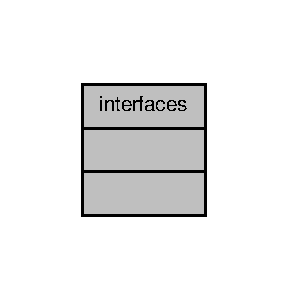
\includegraphics[width=138pt]{classinterfaces__coll__graph}
\end{center}
\end{figure}
\subsection*{Data Types}
\begin{DoxyCompactItemize}
\item 
interface \hyperlink{interfaceinterfaces_1_1abort_execution}{abort\-Execution}
\item 
interface \hyperlink{interfaceinterfaces_1_1performances}{performances}
\item 
interface \hyperlink{interfaceinterfaces_1_1warning}{warning}
\end{DoxyCompactItemize}


\subsection{Detailed Description}


Definition at line 35 of file interfaces.\-f90.



The documentation for this module was generated from the following file\-:\begin{DoxyCompactItemize}
\item 
/home/\-Progetti/\-Siat/\-Ottimizzatore/src/\hyperlink{interfaces_8f90}{interfaces.\-f90}\end{DoxyCompactItemize}

\hypertarget{interfacemathtools_1_1interpolation}{\section{mathtools\-:\-:interpolation Interface Reference}
\label{interfacemathtools_1_1interpolation}\index{mathtools\-::interpolation@{mathtools\-::interpolation}}
}


Collaboration diagram for mathtools\-:\-:interpolation\-:\nopagebreak
\begin{figure}[H]
\begin{center}
\leavevmode
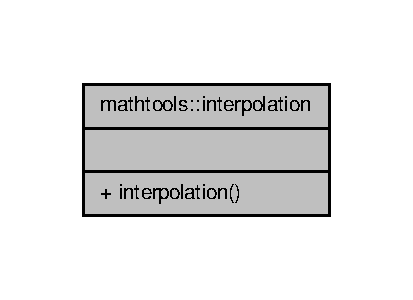
\includegraphics[width=198pt]{interfacemathtools_1_1interpolation__coll__graph}
\end{center}
\end{figure}
\subsection*{Public Member Functions}
\begin{DoxyCompactItemize}
\item 
real(kind=prec) function, \\*
dimension(m) \hyperlink{interfacemathtools_1_1interpolation_a4b6ad870f4e5e805870157ad7d6d7baf}{interpolation} (x\-In, y\-In, n, x\-Out, m, warn)
\end{DoxyCompactItemize}


\subsection{Detailed Description}


Definition at line 41 of file math\-Tools.\-f90.



\subsection{Constructor \& Destructor Documentation}
\hypertarget{interfacemathtools_1_1interpolation_a4b6ad870f4e5e805870157ad7d6d7baf}{\index{mathtools\-::interpolation@{mathtools\-::interpolation}!interpolation@{interpolation}}
\index{interpolation@{interpolation}!mathtools::interpolation@{mathtools\-::interpolation}}
\subsubsection[{interpolation}]{\setlength{\rightskip}{0pt plus 5cm}real(kind = prec) function, dimension(m) mathtools\-::interpolation\-::interpolation (
\begin{DoxyParamCaption}
\item[{real(kind = prec), dimension(n), intent(in)}]{x\-In, }
\item[{real(kind = prec), dimension(n), intent(in)}]{y\-In, }
\item[{integer, intent(in)}]{n, }
\item[{real(kind = prec), dimension(m), intent(in)}]{x\-Out, }
\item[{integer, intent(in)}]{m, }
\item[{integer, dimension(2), intent(in), optional}]{warn}
\end{DoxyParamCaption}
)}}\label{interfacemathtools_1_1interpolation_a4b6ad870f4e5e805870157ad7d6d7baf}


Definition at line 41 of file math\-Tools.\-f90.



The documentation for this interface was generated from the following file\-:\begin{DoxyCompactItemize}
\item 
/home/\-Codici/\-Blink/\-Power\-Manager/src/\hyperlink{math_tools_8f90}{math\-Tools.\-f90}\end{DoxyCompactItemize}

\hypertarget{classmathtools}{\section{mathtools Module Reference}
\label{classmathtools}\index{mathtools@{mathtools}}
}


Collection of interfaces for basic mathematical tools.  




Collaboration diagram for mathtools\-:
\nopagebreak
\begin{figure}[H]
\begin{center}
\leavevmode
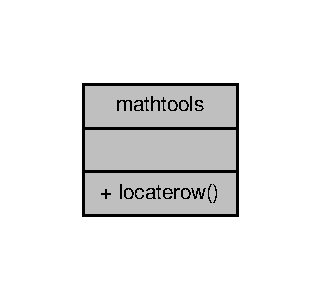
\includegraphics[width=154pt]{classmathtools__coll__graph}
\end{center}
\end{figure}
\subsection*{Data Types}
\begin{DoxyCompactItemize}
\item 
interface \hyperlink{interfacemathtools_1_1interpolation}{interpolation}
\end{DoxyCompactItemize}
\subsection*{Public Member Functions}
\begin{DoxyCompactItemize}
\item 
integer function \hyperlink{classmathtools_a64c72087c0180d1e0cfbd7356d8a1a5a}{locaterow} (row, mat, n, m, error)
\end{DoxyCompactItemize}


\subsection{Detailed Description}
Collection of interfaces for basic mathematical tools. \begin{DoxyAuthor}{Author}
Andrea Facci. 
\end{DoxyAuthor}


Definition at line 36 of file math\-Tools.\-f90.



\subsection{Member Function/\-Subroutine Documentation}
\hypertarget{classmathtools_a64c72087c0180d1e0cfbd7356d8a1a5a}{\index{mathtools@{mathtools}!locaterow@{locaterow}}
\index{locaterow@{locaterow}!mathtools@{mathtools}}
\subsubsection[{locaterow}]{\setlength{\rightskip}{0pt plus 5cm}integer function mathtools\-::locaterow (
\begin{DoxyParamCaption}
\item[{real(kind(1.d0)), dimension(n), intent(in)}]{row, }
\item[{real(kind(1.d0)), dimension(m,n), intent(in)}]{mat, }
\item[{integer, intent(in)}]{n, }
\item[{integer, intent(in)}]{m, }
\item[{logical, intent(out), optional}]{error}
\end{DoxyParamCaption}
)}}\label{classmathtools_a64c72087c0180d1e0cfbd7356d8a1a5a}


Definition at line 51 of file math\-Tools.\-f90.



Referenced by graphtools\-::graphpoints(), and graphtools\-::minpathtopobw().



The documentation for this module was generated from the following file\-:\begin{DoxyCompactItemize}
\item 
/home/andrea/\-Desktop/\-Fortran\-Code\-B\-W/src/\hyperlink{math_tools_8f90}{math\-Tools.\-f90}\end{DoxyCompactItemize}

\hypertarget{interfacefiletools_1_1matrix_read}{\section{filetools\-:\-:matrix\-Read Interface Reference}
\label{interfacefiletools_1_1matrix_read}\index{filetools\-::matrix\-Read@{filetools\-::matrix\-Read}}
}


Collaboration diagram for filetools\-:\-:matrix\-Read\-:\nopagebreak
\begin{figure}[H]
\begin{center}
\leavevmode
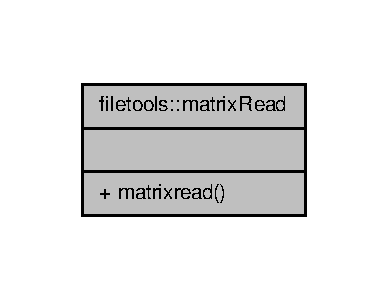
\includegraphics[width=186pt]{interfacefiletools_1_1matrix_read__coll__graph}
\end{center}
\end{figure}
\subsection*{Public Member Functions}
\begin{DoxyCompactItemize}
\item 
character(len=100) function, \\*
dimension(nline) \hyperlink{interfacefiletools_1_1matrix_read_afaa814a69eb7a257ba058ab3ff0aa713}{matrixread} (the\-Unit, nline, first\-\_\-, last\-\_\-)
\end{DoxyCompactItemize}


\subsection{Detailed Description}


Definition at line 101 of file file\-Tools.\-f90.



\subsection{Member Function/\-Subroutine Documentation}
\hypertarget{interfacefiletools_1_1matrix_read_afaa814a69eb7a257ba058ab3ff0aa713}{\index{filetools\-::matrix\-Read@{filetools\-::matrix\-Read}!matrixread@{matrixread}}
\index{matrixread@{matrixread}!filetools::matrixRead@{filetools\-::matrix\-Read}}
\subsubsection[{matrixread}]{\setlength{\rightskip}{0pt plus 5cm}character(len=100) function, dimension(nline) filetools\-::matrix\-Read\-::matrixread (
\begin{DoxyParamCaption}
\item[{integer, intent(in)}]{the\-Unit, }
\item[{integer, intent(in)}]{nline, }
\item[{character(len=1), optional}]{first\-\_\-, }
\item[{character(len=1), optional}]{last\-\_\-}
\end{DoxyParamCaption}
)}}\label{interfacefiletools_1_1matrix_read_afaa814a69eb7a257ba058ab3ff0aa713}


Definition at line 101 of file file\-Tools.\-f90.



The documentation for this interface was generated from the following file\-:\begin{DoxyCompactItemize}
\item 
/home/\-Codici/\-Blink/\-Power\-Manager/src/\hyperlink{file_tools_8f90}{file\-Tools.\-f90}\end{DoxyCompactItemize}

\hypertarget{classmyarithmetic}{\section{myarithmetic Module Reference}
\label{classmyarithmetic}\index{myarithmetic@{myarithmetic}}
}


Creates and detects Na\-N.  




Collaboration diagram for myarithmetic\-:\nopagebreak
\begin{figure}[H]
\begin{center}
\leavevmode
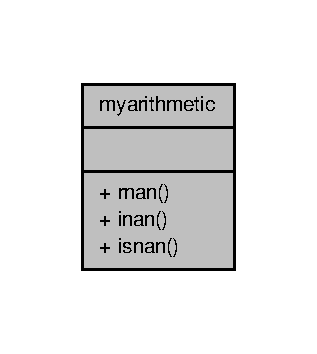
\includegraphics[width=152pt]{classmyarithmetic__coll__graph}
\end{center}
\end{figure}
\subsection*{Public Member Functions}
\begin{DoxyCompactItemize}
\item 
real(kind=prec) function \hyperlink{classmyarithmetic_a227377a7c2675f5faa77ba3c8bc05ec9}{rnan} (x)
\begin{DoxyCompactList}\small\item\em Creates Na\-N. \end{DoxyCompactList}\item 
integer function \hyperlink{classmyarithmetic_a13e401cc199f6d40533cae2c20fac922}{inan} (x)
\begin{DoxyCompactList}\small\item\em Creates Na\-N. \end{DoxyCompactList}\item 
logical function \hyperlink{classmyarithmetic_ac0dec559e69eb7ec762b2eee93884e0f}{isnan} (x)
\begin{DoxyCompactList}\small\item\em Detects Na\-Ns. \end{DoxyCompactList}\end{DoxyCompactItemize}


\subsection{Detailed Description}
This module collects some subroutine useful to create and detect Na\-Ns. It trys to imitate the I\-E\-E\-E\-\_\-\-A\-R\-I\-T\-H\-M\-E\-T\-I\-C module that unfortunately is still not available for the gfortran compiler. \begin{DoxyAuthor}{Author}

\end{DoxyAuthor}


Definition at line 36 of file my\-Arithmetic.\-f90.



\subsection{Member Function/\-Subroutine Documentation}
\hypertarget{classmyarithmetic_a13e401cc199f6d40533cae2c20fac922}{\index{myarithmetic@{myarithmetic}!inan@{inan}}
\index{inan@{inan}!myarithmetic@{myarithmetic}}
\subsubsection[{inan}]{\setlength{\rightskip}{0pt plus 5cm}integer function myarithmetic\-::inan (
\begin{DoxyParamCaption}
\item[{integer, intent(in)}]{x}
\end{DoxyParamCaption}
)}}\label{classmyarithmetic_a13e401cc199f6d40533cae2c20fac922}
Creates a Na\-N to be associated to an integer, variable. 
\begin{DoxyParams}[1]{Parameters}
\mbox{\tt in}  & {\em x} & random integer number. \\
\hline
\end{DoxyParams}
\begin{DoxyAuthor}{Author}
Andrea Facci. 
\end{DoxyAuthor}


Definition at line 61 of file my\-Arithmetic.\-f90.

\hypertarget{classmyarithmetic_ac0dec559e69eb7ec762b2eee93884e0f}{\index{myarithmetic@{myarithmetic}!isnan@{isnan}}
\index{isnan@{isnan}!myarithmetic@{myarithmetic}}
\subsubsection[{isnan}]{\setlength{\rightskip}{0pt plus 5cm}logical function myarithmetic\-::isnan (
\begin{DoxyParamCaption}
\item[{}]{x}
\end{DoxyParamCaption}
)}}\label{classmyarithmetic_ac0dec559e69eb7ec762b2eee93884e0f}
This subroutine determine if a value is Na\-N. 
\begin{DoxyParams}[1]{Parameters}
\mbox{\tt in}  & {\em x} & the value to be tested. \\
\hline
\end{DoxyParams}
\begin{DoxyAuthor}{Author}
Andrea Facci 
\end{DoxyAuthor}


Definition at line 72 of file my\-Arithmetic.\-f90.

\hypertarget{classmyarithmetic_a227377a7c2675f5faa77ba3c8bc05ec9}{\index{myarithmetic@{myarithmetic}!rnan@{rnan}}
\index{rnan@{rnan}!myarithmetic@{myarithmetic}}
\subsubsection[{rnan}]{\setlength{\rightskip}{0pt plus 5cm}real(kind = prec) function myarithmetic\-::rnan (
\begin{DoxyParamCaption}
\item[{real(kind = prec), intent(in)}]{x}
\end{DoxyParamCaption}
)}}\label{classmyarithmetic_a227377a7c2675f5faa77ba3c8bc05ec9}
Creates a Na\-N to be associated to a real, double precition variable. 
\begin{DoxyParams}[1]{Parameters}
\mbox{\tt in}  & {\em x} & random double precision number. \\
\hline
\end{DoxyParams}
\begin{DoxyAuthor}{Author}
Andrea Facci. 
\end{DoxyAuthor}


Definition at line 47 of file my\-Arithmetic.\-f90.



Referenced by graphtools\-::allcombin(), buildplantrev(), readboiler(), readchillers(), readenv(), and readtrigen().



The documentation for this module was generated from the following file\-:\begin{DoxyCompactItemize}
\item 
/home/\-Codici/\-Blink/\-Power\-Manager/src/\hyperlink{my_arithmetic_8f90}{my\-Arithmetic.\-f90}\end{DoxyCompactItemize}

\hypertarget{interfacegraphtools_1_1obj_function}{\section{graphtools\-:\-:obj\-Function Interface Reference}
\label{interfacegraphtools_1_1obj_function}\index{graphtools\-::obj\-Function@{graphtools\-::obj\-Function}}
}


Collaboration diagram for graphtools\-:\-:obj\-Function\-:\nopagebreak
\begin{figure}[H]
\begin{center}
\leavevmode
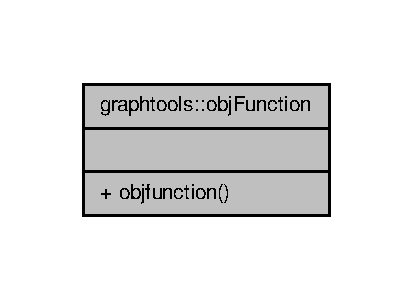
\includegraphics[width=198pt]{interfacegraphtools_1_1obj_function__coll__graph}
\end{center}
\end{figure}
\subsection*{Public Member Functions}
\begin{DoxyCompactItemize}
\item 
real(kind=prec) function \hyperlink{interfacegraphtools_1_1obj_function_aff21e5d518d88e2ef9d4bb3eae3b8066}{objfunction} (c, t, obj)
\end{DoxyCompactItemize}


\subsection{Detailed Description}


Definition at line 61 of file graph\-Tools.\-f90.



\subsection{Member Function/\-Subroutine Documentation}
\hypertarget{interfacegraphtools_1_1obj_function_aff21e5d518d88e2ef9d4bb3eae3b8066}{\index{graphtools\-::obj\-Function@{graphtools\-::obj\-Function}!objfunction@{objfunction}}
\index{objfunction@{objfunction}!graphtools::objFunction@{graphtools\-::obj\-Function}}
\subsubsection[{objfunction}]{\setlength{\rightskip}{0pt plus 5cm}real(kind = prec) function graphtools\-::obj\-Function\-::objfunction (
\begin{DoxyParamCaption}
\item[{integer, dimension(nm), intent(in)}]{c, }
\item[{integer, intent(in)}]{t, }
\item[{character(len=100), intent(in)}]{obj}
\end{DoxyParamCaption}
)}}\label{interfacegraphtools_1_1obj_function_aff21e5d518d88e2ef9d4bb3eae3b8066}


Definition at line 61 of file graph\-Tools.\-f90.



The documentation for this interface was generated from the following file\-:\begin{DoxyCompactItemize}
\item 
/home/\-Codici/\-Blink/\-Power\-Manager/src/\hyperlink{graph_tools_8f90}{graph\-Tools.\-f90}\end{DoxyCompactItemize}

\hypertarget{classplantvar}{\section{plantvar Module Reference}
\label{classplantvar}\index{plantvar@{plantvar}}
}


collection of variables relative to the power plant structure.  




Collaboration diagram for plantvar\-:\nopagebreak
\begin{figure}[H]
\begin{center}
\leavevmode
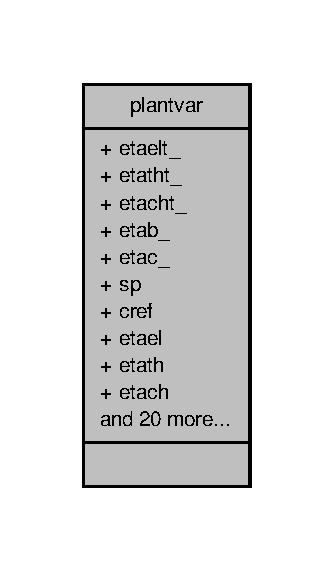
\includegraphics[width=160pt]{classplantvar__coll__graph}
\end{center}
\end{figure}
\subsection*{Public Attributes}
\begin{DoxyCompactItemize}
\item 
real(kind=prec), dimension(\-:,\-:), \\*
allocatable \hyperlink{classplantvar_a42c8e330560c87b991b46be04c40a03d}{etaelt\-\_\-}
\item 
real(kind=prec), dimension(\-:,\-:), \\*
allocatable \hyperlink{classplantvar_a355b18c048762925b750fe247a09c4cd}{etatht\-\_\-}
\item 
real(kind=prec), dimension(\-:,\-:), \\*
allocatable \hyperlink{classplantvar_a1bfe35beb70f107ed930740d7ce7189a}{etacht\-\_\-}
\item 
real(kind=prec), dimension(\-:,\-:), \\*
allocatable \hyperlink{classplantvar_a4307773fae45ef7c05c590189ae40c32}{etab\-\_\-}
\item 
real(kind=prec), dimension(\-:,\-:), \\*
allocatable \hyperlink{classplantvar_ab3e228857f49d79572bc7071e650ae33}{etac\-\_\-}
\item 
real(kind=prec), dimension(\-:,\-:), \\*
allocatable \hyperlink{classplantvar_a0ecfac9070622328232608ce808ede2b}{sp}
\item 
real(kind=prec), dimension(\-:,\-:), \\*
allocatable \hyperlink{classplantvar_a5ddb9d753dc518aed9d34c9e1f5335e0}{cref}
\item 
real(kind=prec), dimension(\-:,\-:,\-:), \\*
allocatable \hyperlink{classplantvar_a187eaf8e3b46428daf4b89db350aa0f1}{envcorr}
\item 
real(kind=prec), dimension(\-:,\-:), \\*
allocatable \hyperlink{classplantvar_a1a1a32a309c970c5ccccda52cbc92e36}{etael}
\item 
real(kind=prec), dimension(\-:,\-:), \\*
allocatable \hyperlink{classplantvar_a226f4150db308d7f4c46da8f297127af}{etath}
\item 
real(kind=prec), dimension(\-:,\-:), \\*
allocatable \hyperlink{classplantvar_a1bae392336fb8d7f0376c7e98163003e}{etach}
\item 
real(kind=prec), dimension(\-:,\-:), \\*
allocatable \hyperlink{classplantvar_aade5aa28513690acf2cf215b0dc1acd2}{timevinc}
\item 
integer, dimension(\-:,\-:), \\*
allocatable \hyperlink{classplantvar_a01620e31bb05f1443908f0bff75215a4}{cr}
\item 
real(kind=prec), dimension(\-:), \\*
allocatable \hyperlink{classplantvar_aab06737bb534df1a69fff1f6f601a72a}{pmax}
\item 
real(kind=prec), dimension(\-:), \\*
allocatable \hyperlink{classplantvar_ae10871bcf2f4379bd15a518a314038de}{dt}
\item 
real(kind=prec), dimension(\-:), \\*
allocatable \hyperlink{classplantvar_af0df4533997b17a1fd69f0c152ce2804}{cf}
\item 
real(kind=prec), dimension(\-:), \\*
allocatable \hyperlink{classplantvar_a8c41db489c4d6b494849ab3c82833e29}{lhv}
\item 
real(kind=prec), dimension(\-:), \\*
allocatable \hyperlink{classplantvar_a2e95a86439f2372f77360c8ba1efaaff}{onoffcost}
\item 
real(kind=prec), dimension(\-:), \\*
allocatable \hyperlink{classplantvar_a70a5a58ce085d08a2b8fb1434ab5862c}{oemcost}
\item 
real(kind=prec), dimension(\-:), \\*
allocatable \hyperlink{classplantvar_aa1e10cfba7b7a224f760c1087d2add6d}{minuptime}
\item 
real(kind=prec), dimension(\-:), \\*
allocatable \hyperlink{classplantvar_a9320c1f8ded834439390cb5602c19863}{mindowntime}
\item 
real(kind=prec), dimension(\-:), \\*
allocatable \hyperlink{classplantvar_adae0478dc0dc873750b3f2ff1cd17f47}{pef}
\item 
real(kind=prec), dimension(\-:), \\*
allocatable \hyperlink{classplantvar_a5f4279bfe683122d1505b7df5897ac45}{pecon}
\item 
real(kind=prec), dimension(\-:), \\*
allocatable \hyperlink{classplantvar_abcd233bb37be100040f7c48ba5700daa}{soc}
\item 
real(kind=prec), dimension(\-:), \\*
allocatable \hyperlink{classplantvar_a9cdc1767d27c7362b6c33bc24fbe79ed}{socth}
\item 
real(kind=prec), dimension(\-:), \\*
allocatable \hyperlink{classplantvar_a325e0974aedb888a4814e7d9479c67d3}{socel}
\item 
real(kind=prec), dimension(\-:), \\*
allocatable \hyperlink{classplantvar_a52a6a33ef0efbd1e6b19c59c683db54a}{esoc}
\item 
character(len=4), dimension(\-:), \\*
allocatable \hyperlink{classplantvar_a8b75644cc6f0b1728b0fdcd7c575c177}{pes}
\item 
integer \hyperlink{classplantvar_a1301bcb36aec6c118be8c084932de099}{nsptot}
\item 
integer \hyperlink{classplantvar_a137041d7f1c30cc7d248b9ada4feab69}{nm}
\item 
integer \hyperlink{classplantvar_a56d8f60e631d2b0dc2d7a0252a49e80e}{nm0}
\item 
integer \hyperlink{classplantvar_ac56a3422e256b7cdcc55623af8ba6c7b}{nsoc}
\item 
integer \hyperlink{classplantvar_a56078fb4f499089dd81db61a9e8dfc0f}{nsocel}
\item 
integer, dimension(5) \hyperlink{classplantvar_ab7276bde0d7595d7ce2ef0470ad21ca9}{is}
\item 
integer, dimension(5) \hyperlink{classplantvar_afa98042e93464d6b9c62a51103cd299f}{ie}
\item 
integer, dimension(\-:), allocatable \hyperlink{classplantvar_a16e98f1a836d4de3e5436365e77441b0}{nsp}
\item 
integer, dimension(\-:), allocatable \hyperlink{classplantvar_a019098844671b06b71ae0b76aa3d4fa8}{ntv}
\item 
integer, dimension(\-:), allocatable \hyperlink{classplantvar_ac5590ecfa29690829feb06fd8c1eb839}{esource}
\item 
character(len=50), dimension(\-:), \\*
allocatable \hyperlink{classplantvar_a4de39d7f2e55534eeac1a570bf8d30ff}{tec}
\item 
real(kind=prec), dimension(\-:), \\*
allocatable \hyperlink{classplantvar_ae2c75e1880b14179e8c96c8bd209f26d}{sunel}
\item 
real(kind=prec), dimension(\-:), \\*
allocatable \hyperlink{classplantvar_a1de4d45e17d60dcfca28b6bd17e74e05}{sunth}
\item 
real(kind=prec), dimension(\-:), \\*
allocatable \hyperlink{classplantvar_a90a77172411c06cf156d494ea2902bfd}{windel}
\item 
logical \hyperlink{classplantvar_a269d2dde89a5632bf0e3d0162c2368c0}{elstor} = .false.
\item 
integer, parameter \hyperlink{classplantvar_ae20b71682087261a45478790df439eb9}{it} = 1
\item 
integer, parameter \hyperlink{classplantvar_a234a52fa723b1234d3725b82c81dad0f}{ib} = 2
\item 
integer, parameter \hyperlink{classplantvar_a395505b74fbf30b4c496601cbd47a64b}{ic} = 3
\item 
integer, parameter \hyperlink{classplantvar_aaa8d59ae7b5ae7303a9b5bd17499ce56}{its} = 4
\item 
integer, parameter \hyperlink{classplantvar_afd5b160dbbf007015da33b4011f36c83}{ies} = 5
\end{DoxyCompactItemize}


\subsection{Detailed Description}
collection of variables relative to the power plant structure. \begin{DoxyAuthor}{Author}

\end{DoxyAuthor}


Definition at line 35 of file plant\-Var.\-f90.



\subsection{Member Data Documentation}
\hypertarget{classplantvar_af0df4533997b17a1fd69f0c152ce2804}{\index{plantvar@{plantvar}!cf@{cf}}
\index{cf@{cf}!plantvar@{plantvar}}
\subsubsection[{cf}]{\setlength{\rightskip}{0pt plus 5cm}real(kind = prec), dimension(\-:), allocatable plantvar\-::cf}}\label{classplantvar_af0df4533997b17a1fd69f0c152ce2804}


Definition at line 46 of file plant\-Var.\-f90.

\hypertarget{classplantvar_a01620e31bb05f1443908f0bff75215a4}{\index{plantvar@{plantvar}!cr@{cr}}
\index{cr@{cr}!plantvar@{plantvar}}
\subsubsection[{cr}]{\setlength{\rightskip}{0pt plus 5cm}integer, dimension(\-:,\-:), allocatable plantvar\-::cr}}\label{classplantvar_a01620e31bb05f1443908f0bff75215a4}


Definition at line 45 of file plant\-Var.\-f90.

\hypertarget{classplantvar_a5ddb9d753dc518aed9d34c9e1f5335e0}{\index{plantvar@{plantvar}!cref@{cref}}
\index{cref@{cref}!plantvar@{plantvar}}
\subsubsection[{cref}]{\setlength{\rightskip}{0pt plus 5cm}real(kind = prec), dimension(\-:,\-:), allocatable plantvar\-::cref}}\label{classplantvar_a5ddb9d753dc518aed9d34c9e1f5335e0}


Definition at line 41 of file plant\-Var.\-f90.

\hypertarget{classplantvar_ae10871bcf2f4379bd15a518a314038de}{\index{plantvar@{plantvar}!dt@{dt}}
\index{dt@{dt}!plantvar@{plantvar}}
\subsubsection[{dt}]{\setlength{\rightskip}{0pt plus 5cm}real(kind = prec), dimension(\-:), allocatable plantvar\-::dt}}\label{classplantvar_ae10871bcf2f4379bd15a518a314038de}


Definition at line 46 of file plant\-Var.\-f90.

\hypertarget{classplantvar_a269d2dde89a5632bf0e3d0162c2368c0}{\index{plantvar@{plantvar}!elstor@{elstor}}
\index{elstor@{elstor}!plantvar@{plantvar}}
\subsubsection[{elstor}]{\setlength{\rightskip}{0pt plus 5cm}logical plantvar\-::elstor = .false.}}\label{classplantvar_a269d2dde89a5632bf0e3d0162c2368c0}


Definition at line 54 of file plant\-Var.\-f90.

\hypertarget{classplantvar_a187eaf8e3b46428daf4b89db350aa0f1}{\index{plantvar@{plantvar}!envcorr@{envcorr}}
\index{envcorr@{envcorr}!plantvar@{plantvar}}
\subsubsection[{envcorr}]{\setlength{\rightskip}{0pt plus 5cm}real(kind = prec), dimension(\-:,\-:,\-:), allocatable plantvar\-::envcorr}}\label{classplantvar_a187eaf8e3b46428daf4b89db350aa0f1}


Definition at line 43 of file plant\-Var.\-f90.

\hypertarget{classplantvar_a52a6a33ef0efbd1e6b19c59c683db54a}{\index{plantvar@{plantvar}!esoc@{esoc}}
\index{esoc@{esoc}!plantvar@{plantvar}}
\subsubsection[{esoc}]{\setlength{\rightskip}{0pt plus 5cm}real(kind = prec), dimension(\-:), allocatable plantvar\-::esoc}}\label{classplantvar_a52a6a33ef0efbd1e6b19c59c683db54a}


Definition at line 46 of file plant\-Var.\-f90.

\hypertarget{classplantvar_ac5590ecfa29690829feb06fd8c1eb839}{\index{plantvar@{plantvar}!esource@{esource}}
\index{esource@{esource}!plantvar@{plantvar}}
\subsubsection[{esource}]{\setlength{\rightskip}{0pt plus 5cm}integer, dimension(\-:), allocatable plantvar\-::esource}}\label{classplantvar_ac5590ecfa29690829feb06fd8c1eb839}


Definition at line 51 of file plant\-Var.\-f90.

\hypertarget{classplantvar_a4307773fae45ef7c05c590189ae40c32}{\index{plantvar@{plantvar}!etab\-\_\-@{etab\-\_\-}}
\index{etab\-\_\-@{etab\-\_\-}!plantvar@{plantvar}}
\subsubsection[{etab\-\_\-}]{\setlength{\rightskip}{0pt plus 5cm}real(kind = prec), dimension(\-:,\-:), allocatable plantvar\-::etab\-\_\-}}\label{classplantvar_a4307773fae45ef7c05c590189ae40c32}


Definition at line 41 of file plant\-Var.\-f90.

\hypertarget{classplantvar_ab3e228857f49d79572bc7071e650ae33}{\index{plantvar@{plantvar}!etac\-\_\-@{etac\-\_\-}}
\index{etac\-\_\-@{etac\-\_\-}!plantvar@{plantvar}}
\subsubsection[{etac\-\_\-}]{\setlength{\rightskip}{0pt plus 5cm}real(kind = prec), dimension(\-:,\-:), allocatable plantvar\-::etac\-\_\-}}\label{classplantvar_ab3e228857f49d79572bc7071e650ae33}


Definition at line 41 of file plant\-Var.\-f90.

\hypertarget{classplantvar_a1bae392336fb8d7f0376c7e98163003e}{\index{plantvar@{plantvar}!etach@{etach}}
\index{etach@{etach}!plantvar@{plantvar}}
\subsubsection[{etach}]{\setlength{\rightskip}{0pt plus 5cm}real(kind = prec), dimension(\-:,\-:), allocatable plantvar\-::etach}}\label{classplantvar_a1bae392336fb8d7f0376c7e98163003e}


Definition at line 44 of file plant\-Var.\-f90.

\hypertarget{classplantvar_a1bfe35beb70f107ed930740d7ce7189a}{\index{plantvar@{plantvar}!etacht\-\_\-@{etacht\-\_\-}}
\index{etacht\-\_\-@{etacht\-\_\-}!plantvar@{plantvar}}
\subsubsection[{etacht\-\_\-}]{\setlength{\rightskip}{0pt plus 5cm}real(kind = prec), dimension(\-:,\-:), allocatable plantvar\-::etacht\-\_\-}}\label{classplantvar_a1bfe35beb70f107ed930740d7ce7189a}


Definition at line 41 of file plant\-Var.\-f90.

\hypertarget{classplantvar_a1a1a32a309c970c5ccccda52cbc92e36}{\index{plantvar@{plantvar}!etael@{etael}}
\index{etael@{etael}!plantvar@{plantvar}}
\subsubsection[{etael}]{\setlength{\rightskip}{0pt plus 5cm}real(kind = prec), dimension(\-:,\-:), allocatable plantvar\-::etael}}\label{classplantvar_a1a1a32a309c970c5ccccda52cbc92e36}


Definition at line 44 of file plant\-Var.\-f90.

\hypertarget{classplantvar_a42c8e330560c87b991b46be04c40a03d}{\index{plantvar@{plantvar}!etaelt\-\_\-@{etaelt\-\_\-}}
\index{etaelt\-\_\-@{etaelt\-\_\-}!plantvar@{plantvar}}
\subsubsection[{etaelt\-\_\-}]{\setlength{\rightskip}{0pt plus 5cm}real(kind = prec), dimension(\-:,\-:), allocatable plantvar\-::etaelt\-\_\-}}\label{classplantvar_a42c8e330560c87b991b46be04c40a03d}


Definition at line 41 of file plant\-Var.\-f90.

\hypertarget{classplantvar_a226f4150db308d7f4c46da8f297127af}{\index{plantvar@{plantvar}!etath@{etath}}
\index{etath@{etath}!plantvar@{plantvar}}
\subsubsection[{etath}]{\setlength{\rightskip}{0pt plus 5cm}real(kind = prec), dimension(\-:,\-:), allocatable plantvar\-::etath}}\label{classplantvar_a226f4150db308d7f4c46da8f297127af}


Definition at line 44 of file plant\-Var.\-f90.

\hypertarget{classplantvar_a355b18c048762925b750fe247a09c4cd}{\index{plantvar@{plantvar}!etatht\-\_\-@{etatht\-\_\-}}
\index{etatht\-\_\-@{etatht\-\_\-}!plantvar@{plantvar}}
\subsubsection[{etatht\-\_\-}]{\setlength{\rightskip}{0pt plus 5cm}real(kind = prec), dimension(\-:,\-:), allocatable plantvar\-::etatht\-\_\-}}\label{classplantvar_a355b18c048762925b750fe247a09c4cd}


Definition at line 41 of file plant\-Var.\-f90.

\hypertarget{classplantvar_a234a52fa723b1234d3725b82c81dad0f}{\index{plantvar@{plantvar}!ib@{ib}}
\index{ib@{ib}!plantvar@{plantvar}}
\subsubsection[{ib}]{\setlength{\rightskip}{0pt plus 5cm}integer, parameter plantvar\-::ib = 2}}\label{classplantvar_a234a52fa723b1234d3725b82c81dad0f}


Definition at line 56 of file plant\-Var.\-f90.

\hypertarget{classplantvar_a395505b74fbf30b4c496601cbd47a64b}{\index{plantvar@{plantvar}!ic@{ic}}
\index{ic@{ic}!plantvar@{plantvar}}
\subsubsection[{ic}]{\setlength{\rightskip}{0pt plus 5cm}integer, parameter plantvar\-::ic = 3}}\label{classplantvar_a395505b74fbf30b4c496601cbd47a64b}


Definition at line 56 of file plant\-Var.\-f90.

\hypertarget{classplantvar_afa98042e93464d6b9c62a51103cd299f}{\index{plantvar@{plantvar}!ie@{ie}}
\index{ie@{ie}!plantvar@{plantvar}}
\subsubsection[{ie}]{\setlength{\rightskip}{0pt plus 5cm}integer, dimension(5) plantvar\-::ie}}\label{classplantvar_afa98042e93464d6b9c62a51103cd299f}


Definition at line 50 of file plant\-Var.\-f90.

\hypertarget{classplantvar_afd5b160dbbf007015da33b4011f36c83}{\index{plantvar@{plantvar}!ies@{ies}}
\index{ies@{ies}!plantvar@{plantvar}}
\subsubsection[{ies}]{\setlength{\rightskip}{0pt plus 5cm}integer, parameter plantvar\-::ies = 5}}\label{classplantvar_afd5b160dbbf007015da33b4011f36c83}


Definition at line 56 of file plant\-Var.\-f90.

\hypertarget{classplantvar_ab7276bde0d7595d7ce2ef0470ad21ca9}{\index{plantvar@{plantvar}!is@{is}}
\index{is@{is}!plantvar@{plantvar}}
\subsubsection[{is}]{\setlength{\rightskip}{0pt plus 5cm}integer, dimension(5) plantvar\-::is}}\label{classplantvar_ab7276bde0d7595d7ce2ef0470ad21ca9}


Definition at line 50 of file plant\-Var.\-f90.

\hypertarget{classplantvar_ae20b71682087261a45478790df439eb9}{\index{plantvar@{plantvar}!it@{it}}
\index{it@{it}!plantvar@{plantvar}}
\subsubsection[{it}]{\setlength{\rightskip}{0pt plus 5cm}integer, parameter plantvar\-::it = 1}}\label{classplantvar_ae20b71682087261a45478790df439eb9}


Definition at line 56 of file plant\-Var.\-f90.

\hypertarget{classplantvar_aaa8d59ae7b5ae7303a9b5bd17499ce56}{\index{plantvar@{plantvar}!its@{its}}
\index{its@{its}!plantvar@{plantvar}}
\subsubsection[{its}]{\setlength{\rightskip}{0pt plus 5cm}integer, parameter plantvar\-::its = 4}}\label{classplantvar_aaa8d59ae7b5ae7303a9b5bd17499ce56}


Definition at line 56 of file plant\-Var.\-f90.

\hypertarget{classplantvar_a8c41db489c4d6b494849ab3c82833e29}{\index{plantvar@{plantvar}!lhv@{lhv}}
\index{lhv@{lhv}!plantvar@{plantvar}}
\subsubsection[{lhv}]{\setlength{\rightskip}{0pt plus 5cm}real(kind = prec), dimension(\-:), allocatable plantvar\-::lhv}}\label{classplantvar_a8c41db489c4d6b494849ab3c82833e29}


Definition at line 46 of file plant\-Var.\-f90.

\hypertarget{classplantvar_a9320c1f8ded834439390cb5602c19863}{\index{plantvar@{plantvar}!mindowntime@{mindowntime}}
\index{mindowntime@{mindowntime}!plantvar@{plantvar}}
\subsubsection[{mindowntime}]{\setlength{\rightskip}{0pt plus 5cm}real(kind = prec), dimension(\-:), allocatable plantvar\-::mindowntime}}\label{classplantvar_a9320c1f8ded834439390cb5602c19863}


Definition at line 46 of file plant\-Var.\-f90.

\hypertarget{classplantvar_aa1e10cfba7b7a224f760c1087d2add6d}{\index{plantvar@{plantvar}!minuptime@{minuptime}}
\index{minuptime@{minuptime}!plantvar@{plantvar}}
\subsubsection[{minuptime}]{\setlength{\rightskip}{0pt plus 5cm}real(kind = prec), dimension(\-:), allocatable plantvar\-::minuptime}}\label{classplantvar_aa1e10cfba7b7a224f760c1087d2add6d}


Definition at line 46 of file plant\-Var.\-f90.

\hypertarget{classplantvar_a137041d7f1c30cc7d248b9ada4feab69}{\index{plantvar@{plantvar}!nm@{nm}}
\index{nm@{nm}!plantvar@{plantvar}}
\subsubsection[{nm}]{\setlength{\rightskip}{0pt plus 5cm}integer plantvar\-::nm}}\label{classplantvar_a137041d7f1c30cc7d248b9ada4feab69}


Definition at line 49 of file plant\-Var.\-f90.

\hypertarget{classplantvar_a56d8f60e631d2b0dc2d7a0252a49e80e}{\index{plantvar@{plantvar}!nm0@{nm0}}
\index{nm0@{nm0}!plantvar@{plantvar}}
\subsubsection[{nm0}]{\setlength{\rightskip}{0pt plus 5cm}integer plantvar\-::nm0}}\label{classplantvar_a56d8f60e631d2b0dc2d7a0252a49e80e}


Definition at line 49 of file plant\-Var.\-f90.

\hypertarget{classplantvar_ac56a3422e256b7cdcc55623af8ba6c7b}{\index{plantvar@{plantvar}!nsoc@{nsoc}}
\index{nsoc@{nsoc}!plantvar@{plantvar}}
\subsubsection[{nsoc}]{\setlength{\rightskip}{0pt plus 5cm}integer plantvar\-::nsoc}}\label{classplantvar_ac56a3422e256b7cdcc55623af8ba6c7b}


Definition at line 49 of file plant\-Var.\-f90.

\hypertarget{classplantvar_a56078fb4f499089dd81db61a9e8dfc0f}{\index{plantvar@{plantvar}!nsocel@{nsocel}}
\index{nsocel@{nsocel}!plantvar@{plantvar}}
\subsubsection[{nsocel}]{\setlength{\rightskip}{0pt plus 5cm}integer plantvar\-::nsocel}}\label{classplantvar_a56078fb4f499089dd81db61a9e8dfc0f}


Definition at line 49 of file plant\-Var.\-f90.

\hypertarget{classplantvar_a16e98f1a836d4de3e5436365e77441b0}{\index{plantvar@{plantvar}!nsp@{nsp}}
\index{nsp@{nsp}!plantvar@{plantvar}}
\subsubsection[{nsp}]{\setlength{\rightskip}{0pt plus 5cm}integer, dimension(\-:), allocatable plantvar\-::nsp}}\label{classplantvar_a16e98f1a836d4de3e5436365e77441b0}


Definition at line 51 of file plant\-Var.\-f90.

\hypertarget{classplantvar_a1301bcb36aec6c118be8c084932de099}{\index{plantvar@{plantvar}!nsptot@{nsptot}}
\index{nsptot@{nsptot}!plantvar@{plantvar}}
\subsubsection[{nsptot}]{\setlength{\rightskip}{0pt plus 5cm}integer plantvar\-::nsptot}}\label{classplantvar_a1301bcb36aec6c118be8c084932de099}


Definition at line 49 of file plant\-Var.\-f90.

\hypertarget{classplantvar_a019098844671b06b71ae0b76aa3d4fa8}{\index{plantvar@{plantvar}!ntv@{ntv}}
\index{ntv@{ntv}!plantvar@{plantvar}}
\subsubsection[{ntv}]{\setlength{\rightskip}{0pt plus 5cm}integer, dimension(\-:), allocatable plantvar\-::ntv}}\label{classplantvar_a019098844671b06b71ae0b76aa3d4fa8}


Definition at line 51 of file plant\-Var.\-f90.

\hypertarget{classplantvar_a70a5a58ce085d08a2b8fb1434ab5862c}{\index{plantvar@{plantvar}!oemcost@{oemcost}}
\index{oemcost@{oemcost}!plantvar@{plantvar}}
\subsubsection[{oemcost}]{\setlength{\rightskip}{0pt plus 5cm}real(kind = prec), dimension(\-:), allocatable plantvar\-::oemcost}}\label{classplantvar_a70a5a58ce085d08a2b8fb1434ab5862c}


Definition at line 46 of file plant\-Var.\-f90.

\hypertarget{classplantvar_a2e95a86439f2372f77360c8ba1efaaff}{\index{plantvar@{plantvar}!onoffcost@{onoffcost}}
\index{onoffcost@{onoffcost}!plantvar@{plantvar}}
\subsubsection[{onoffcost}]{\setlength{\rightskip}{0pt plus 5cm}real(kind = prec), dimension(\-:), allocatable plantvar\-::onoffcost}}\label{classplantvar_a2e95a86439f2372f77360c8ba1efaaff}


Definition at line 46 of file plant\-Var.\-f90.

\hypertarget{classplantvar_a5f4279bfe683122d1505b7df5897ac45}{\index{plantvar@{plantvar}!pecon@{pecon}}
\index{pecon@{pecon}!plantvar@{plantvar}}
\subsubsection[{pecon}]{\setlength{\rightskip}{0pt plus 5cm}real(kind = prec), dimension(\-:), allocatable plantvar\-::pecon}}\label{classplantvar_a5f4279bfe683122d1505b7df5897ac45}


Definition at line 46 of file plant\-Var.\-f90.

\hypertarget{classplantvar_adae0478dc0dc873750b3f2ff1cd17f47}{\index{plantvar@{plantvar}!pef@{pef}}
\index{pef@{pef}!plantvar@{plantvar}}
\subsubsection[{pef}]{\setlength{\rightskip}{0pt plus 5cm}real(kind = prec), dimension(\-:), allocatable plantvar\-::pef}}\label{classplantvar_adae0478dc0dc873750b3f2ff1cd17f47}


Definition at line 46 of file plant\-Var.\-f90.

\hypertarget{classplantvar_a8b75644cc6f0b1728b0fdcd7c575c177}{\index{plantvar@{plantvar}!pes@{pes}}
\index{pes@{pes}!plantvar@{plantvar}}
\subsubsection[{pes}]{\setlength{\rightskip}{0pt plus 5cm}character(len=4), dimension(\-:), allocatable plantvar\-::pes}}\label{classplantvar_a8b75644cc6f0b1728b0fdcd7c575c177}


Definition at line 48 of file plant\-Var.\-f90.

\hypertarget{classplantvar_aab06737bb534df1a69fff1f6f601a72a}{\index{plantvar@{plantvar}!pmax@{pmax}}
\index{pmax@{pmax}!plantvar@{plantvar}}
\subsubsection[{pmax}]{\setlength{\rightskip}{0pt plus 5cm}real(kind = prec), dimension(\-:), allocatable plantvar\-::pmax}}\label{classplantvar_aab06737bb534df1a69fff1f6f601a72a}


Definition at line 46 of file plant\-Var.\-f90.

\hypertarget{classplantvar_abcd233bb37be100040f7c48ba5700daa}{\index{plantvar@{plantvar}!soc@{soc}}
\index{soc@{soc}!plantvar@{plantvar}}
\subsubsection[{soc}]{\setlength{\rightskip}{0pt plus 5cm}real(kind = prec), dimension(\-:), allocatable plantvar\-::soc}}\label{classplantvar_abcd233bb37be100040f7c48ba5700daa}


Definition at line 46 of file plant\-Var.\-f90.

\hypertarget{classplantvar_a325e0974aedb888a4814e7d9479c67d3}{\index{plantvar@{plantvar}!socel@{socel}}
\index{socel@{socel}!plantvar@{plantvar}}
\subsubsection[{socel}]{\setlength{\rightskip}{0pt plus 5cm}real(kind = prec), dimension(\-:), allocatable plantvar\-::socel}}\label{classplantvar_a325e0974aedb888a4814e7d9479c67d3}


Definition at line 46 of file plant\-Var.\-f90.

\hypertarget{classplantvar_a9cdc1767d27c7362b6c33bc24fbe79ed}{\index{plantvar@{plantvar}!socth@{socth}}
\index{socth@{socth}!plantvar@{plantvar}}
\subsubsection[{socth}]{\setlength{\rightskip}{0pt plus 5cm}real(kind = prec), dimension(\-:), allocatable plantvar\-::socth}}\label{classplantvar_a9cdc1767d27c7362b6c33bc24fbe79ed}


Definition at line 46 of file plant\-Var.\-f90.

\hypertarget{classplantvar_a0ecfac9070622328232608ce808ede2b}{\index{plantvar@{plantvar}!sp@{sp}}
\index{sp@{sp}!plantvar@{plantvar}}
\subsubsection[{sp}]{\setlength{\rightskip}{0pt plus 5cm}real(kind = prec), dimension(\-:,\-:), allocatable plantvar\-::sp}}\label{classplantvar_a0ecfac9070622328232608ce808ede2b}


Definition at line 41 of file plant\-Var.\-f90.

\hypertarget{classplantvar_ae2c75e1880b14179e8c96c8bd209f26d}{\index{plantvar@{plantvar}!sunel@{sunel}}
\index{sunel@{sunel}!plantvar@{plantvar}}
\subsubsection[{sunel}]{\setlength{\rightskip}{0pt plus 5cm}real(kind=prec), dimension(\-:), allocatable plantvar\-::sunel}}\label{classplantvar_ae2c75e1880b14179e8c96c8bd209f26d}


Definition at line 53 of file plant\-Var.\-f90.

\hypertarget{classplantvar_a1de4d45e17d60dcfca28b6bd17e74e05}{\index{plantvar@{plantvar}!sunth@{sunth}}
\index{sunth@{sunth}!plantvar@{plantvar}}
\subsubsection[{sunth}]{\setlength{\rightskip}{0pt plus 5cm}real(kind=prec), dimension(\-:), allocatable plantvar\-::sunth}}\label{classplantvar_a1de4d45e17d60dcfca28b6bd17e74e05}


Definition at line 53 of file plant\-Var.\-f90.

\hypertarget{classplantvar_a4de39d7f2e55534eeac1a570bf8d30ff}{\index{plantvar@{plantvar}!tec@{tec}}
\index{tec@{tec}!plantvar@{plantvar}}
\subsubsection[{tec}]{\setlength{\rightskip}{0pt plus 5cm}character(len=50), dimension(\-:), allocatable plantvar\-::tec}}\label{classplantvar_a4de39d7f2e55534eeac1a570bf8d30ff}


Definition at line 52 of file plant\-Var.\-f90.

\hypertarget{classplantvar_aade5aa28513690acf2cf215b0dc1acd2}{\index{plantvar@{plantvar}!timevinc@{timevinc}}
\index{timevinc@{timevinc}!plantvar@{plantvar}}
\subsubsection[{timevinc}]{\setlength{\rightskip}{0pt plus 5cm}real(kind = prec), dimension(\-:,\-:), allocatable plantvar\-::timevinc}}\label{classplantvar_aade5aa28513690acf2cf215b0dc1acd2}


Definition at line 44 of file plant\-Var.\-f90.

\hypertarget{classplantvar_a90a77172411c06cf156d494ea2902bfd}{\index{plantvar@{plantvar}!windel@{windel}}
\index{windel@{windel}!plantvar@{plantvar}}
\subsubsection[{windel}]{\setlength{\rightskip}{0pt plus 5cm}real(kind=prec), dimension(\-:), allocatable plantvar\-::windel}}\label{classplantvar_a90a77172411c06cf156d494ea2902bfd}


Definition at line 53 of file plant\-Var.\-f90.



The documentation for this module was generated from the following file\-:\begin{DoxyCompactItemize}
\item 
/home/\-Codici/\-Blink/\-Power\-Manager/src/\hyperlink{plant_var_8f90}{plant\-Var.\-f90}\end{DoxyCompactItemize}

\hypertarget{interfacefiletools_1_1read_keyword}{\section{filetools\-:\-:read\-Keyword Interface Reference}
\label{interfacefiletools_1_1read_keyword}\index{filetools\-::read\-Keyword@{filetools\-::read\-Keyword}}
}


Collaboration diagram for filetools\-:\-:read\-Keyword\-:\nopagebreak
\begin{figure}[H]
\begin{center}
\leavevmode
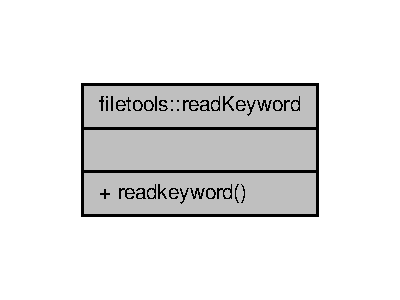
\includegraphics[width=192pt]{interfacefiletools_1_1read_keyword__coll__graph}
\end{center}
\end{figure}
\subsection*{Public Member Functions}
\begin{DoxyCompactItemize}
\item 
subroutine \hyperlink{interfacefiletools_1_1read_keyword_a40ca3283fc0c58b6f9ab7d2d921b6f5a}{readkeyword} (the\-Unit, rew, keyword, value, error, n\-Row)
\end{DoxyCompactItemize}


\subsection{Detailed Description}


Definition at line 166 of file file\-Tools.\-f90.



\subsection{Member Function/\-Subroutine Documentation}
\hypertarget{interfacefiletools_1_1read_keyword_a40ca3283fc0c58b6f9ab7d2d921b6f5a}{\index{filetools\-::read\-Keyword@{filetools\-::read\-Keyword}!readkeyword@{readkeyword}}
\index{readkeyword@{readkeyword}!filetools::readKeyword@{filetools\-::read\-Keyword}}
\subsubsection[{readkeyword}]{\setlength{\rightskip}{0pt plus 5cm}subroutine filetools\-::read\-Keyword\-::readkeyword (
\begin{DoxyParamCaption}
\item[{integer, intent(in)}]{the\-Unit, }
\item[{logical, intent(in), optional}]{rew, }
\item[{character(len=100), intent(out)}]{keyword, }
\item[{character(len=100), intent(out)}]{value, }
\item[{integer, intent(out), optional}]{error, }
\item[{integer, intent(out), optional}]{n\-Row}
\end{DoxyParamCaption}
)}}\label{interfacefiletools_1_1read_keyword_a40ca3283fc0c58b6f9ab7d2d921b6f5a}


Definition at line 166 of file file\-Tools.\-f90.



The documentation for this interface was generated from the following file\-:\begin{DoxyCompactItemize}
\item 
/home/\-Progetti/\-Siat/\-Ottimizzatore/src/\hyperlink{file_tools_8f90}{file\-Tools.\-f90}\end{DoxyCompactItemize}

\hypertarget{interfacefiletools_1_1rew_unit}{\section{filetools\-:\-:rew\-Unit Interface Reference}
\label{interfacefiletools_1_1rew_unit}\index{filetools\-::rew\-Unit@{filetools\-::rew\-Unit}}
}


Collaboration diagram for filetools\-:\-:rew\-Unit\-:\nopagebreak
\begin{figure}[H]
\begin{center}
\leavevmode
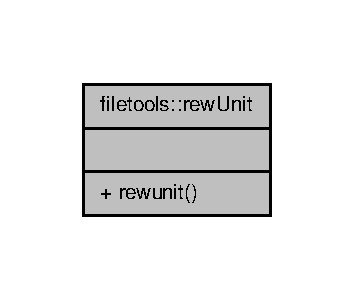
\includegraphics[width=170pt]{interfacefiletools_1_1rew_unit__coll__graph}
\end{center}
\end{figure}
\subsection*{Public Member Functions}
\begin{DoxyCompactItemize}
\item 
subroutine \hyperlink{interfacefiletools_1_1rew_unit_ae40c548f951aab72dc54707581133b08}{rewunit} (the\-Unit, n)
\end{DoxyCompactItemize}


\subsection{Detailed Description}


Definition at line 44 of file file\-Tools.\-f90.



\subsection{Member Function/\-Subroutine Documentation}
\hypertarget{interfacefiletools_1_1rew_unit_ae40c548f951aab72dc54707581133b08}{\index{filetools\-::rew\-Unit@{filetools\-::rew\-Unit}!rewunit@{rewunit}}
\index{rewunit@{rewunit}!filetools::rewUnit@{filetools\-::rew\-Unit}}
\subsubsection[{rewunit}]{\setlength{\rightskip}{0pt plus 5cm}subroutine filetools\-::rew\-Unit\-::rewunit (
\begin{DoxyParamCaption}
\item[{integer, intent(in)}]{the\-Unit, }
\item[{integer, intent(in)}]{n}
\end{DoxyParamCaption}
)}}\label{interfacefiletools_1_1rew_unit_ae40c548f951aab72dc54707581133b08}


Definition at line 44 of file file\-Tools.\-f90.



The documentation for this interface was generated from the following file\-:\begin{DoxyCompactItemize}
\item 
/home/\-Codici/\-Blink/\-Power\-Manager/src/\hyperlink{file_tools_8f90}{file\-Tools.\-f90}\end{DoxyCompactItemize}

\hypertarget{interfacegraphtools_1_1time_constr}{\section{graphtools\-:\-:time\-Constr Interface Reference}
\label{interfacegraphtools_1_1time_constr}\index{graphtools\-::time\-Constr@{graphtools\-::time\-Constr}}
}


Collaboration diagram for graphtools\-:\-:time\-Constr\-:
\nopagebreak
\begin{figure}[H]
\begin{center}
\leavevmode
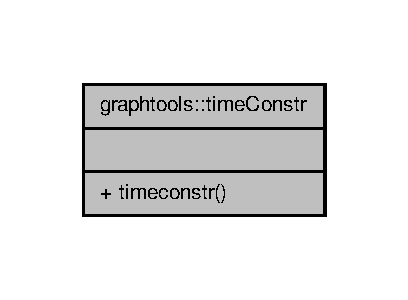
\includegraphics[width=196pt]{interfacegraphtools_1_1time_constr__coll__graph}
\end{center}
\end{figure}
\subsection*{Public Member Functions}
\begin{DoxyCompactItemize}
\item 
logical function \hyperlink{interfacegraphtools_1_1time_constr_a603698c9db0de9269bc3084299e18937}{timeconstr} (cindex, t\-State)
\end{DoxyCompactItemize}


\subsection{Detailed Description}


Definition at line 78 of file graph\-Tools.\-f90.



\subsection{Member Function/\-Subroutine Documentation}
\hypertarget{interfacegraphtools_1_1time_constr_a603698c9db0de9269bc3084299e18937}{\index{graphtools\-::time\-Constr@{graphtools\-::time\-Constr}!timeconstr@{timeconstr}}
\index{timeconstr@{timeconstr}!graphtools::timeConstr@{graphtools\-::time\-Constr}}
\subsubsection[{timeconstr}]{\setlength{\rightskip}{0pt plus 5cm}logical function graphtools\-::time\-Constr\-::timeconstr (
\begin{DoxyParamCaption}
\item[{integer, dimension(nm), intent(in)}]{cindex, }
\item[{real(kind(1.d0)), dimension(nm), intent(in)}]{t\-State}
\end{DoxyParamCaption}
)}}\label{interfacegraphtools_1_1time_constr_a603698c9db0de9269bc3084299e18937}


Definition at line 78 of file graph\-Tools.\-f90.



The documentation for this interface was generated from the following file\-:\begin{DoxyCompactItemize}
\item 
/home/andrea/\-Desktop/\-Fortran\-Code\-B\-W/src/\hyperlink{graph_tools_8f90}{graph\-Tools.\-f90}\end{DoxyCompactItemize}

\hypertarget{interfacefiletools_1_1v_count}{\section{filetools\-:\-:v\-Count Interface Reference}
\label{interfacefiletools_1_1v_count}\index{filetools\-::v\-Count@{filetools\-::v\-Count}}
}


Collaboration diagram for filetools\-:\-:v\-Count\-:\nopagebreak
\begin{figure}[H]
\begin{center}
\leavevmode
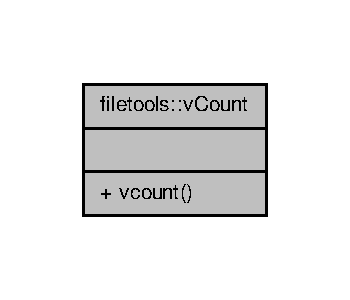
\includegraphics[width=168pt]{interfacefiletools_1_1v_count__coll__graph}
\end{center}
\end{figure}
\subsection*{Public Member Functions}
\begin{DoxyCompactItemize}
\item 
integer function \hyperlink{interfacefiletools_1_1v_count_a96ad9161089f8da6f08078f5417e3d2a}{vcount} (the\-Unit, rew\-\_\-, first\-\_\-, last\-\_\-)
\end{DoxyCompactItemize}


\subsection{Detailed Description}


Definition at line 49 of file file\-Tools.\-f90.



\subsection{Member Function/\-Subroutine Documentation}
\hypertarget{interfacefiletools_1_1v_count_a96ad9161089f8da6f08078f5417e3d2a}{\index{filetools\-::v\-Count@{filetools\-::v\-Count}!vcount@{vcount}}
\index{vcount@{vcount}!filetools::vCount@{filetools\-::v\-Count}}
\subsubsection[{vcount}]{\setlength{\rightskip}{0pt plus 5cm}integer function filetools\-::v\-Count\-::vcount (
\begin{DoxyParamCaption}
\item[{integer, intent(in)}]{the\-Unit, }
\item[{logical, optional}]{rew\-\_\-, }
\item[{character(len=1), intent(in), optional}]{first\-\_\-, }
\item[{character(len=1), intent(in), optional}]{last\-\_\-}
\end{DoxyParamCaption}
)}}\label{interfacefiletools_1_1v_count_a96ad9161089f8da6f08078f5417e3d2a}


Definition at line 49 of file file\-Tools.\-f90.



The documentation for this interface was generated from the following file\-:\begin{DoxyCompactItemize}
\item 
/home/andrea/\-Desktop/\-Fortran\-Code\-B\-W/src/\hyperlink{file_tools_8f90}{file\-Tools.\-f90}\end{DoxyCompactItemize}

\hypertarget{interfaceinterfaces_1_1warning}{\section{interfaces\-:\-:warning Interface Reference}
\label{interfaceinterfaces_1_1warning}\index{interfaces\-::warning@{interfaces\-::warning}}
}


Collaboration diagram for interfaces\-:\-:warning\-:\nopagebreak
\begin{figure}[H]
\begin{center}
\leavevmode
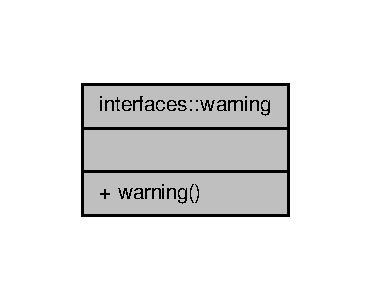
\includegraphics[width=178pt]{interfaceinterfaces_1_1warning__coll__graph}
\end{center}
\end{figure}
\subsection*{Public Member Functions}
\begin{DoxyCompactItemize}
\item 
subroutine \hyperlink{interfaceinterfaces_1_1warning_a167b4a1eeeff911a881c3159e243147d}{warning} (i, j, k, line, word, r1, r2)
\end{DoxyCompactItemize}


\subsection{Detailed Description}


Definition at line 50 of file interfaces.\-f90.



\subsection{Constructor \& Destructor Documentation}
\hypertarget{interfaceinterfaces_1_1warning_a167b4a1eeeff911a881c3159e243147d}{\index{interfaces\-::warning@{interfaces\-::warning}!warning@{warning}}
\index{warning@{warning}!interfaces::warning@{interfaces\-::warning}}
\subsubsection[{warning}]{\setlength{\rightskip}{0pt plus 5cm}subroutine interfaces\-::warning\-::warning (
\begin{DoxyParamCaption}
\item[{integer, intent(in), optional}]{i, }
\item[{integer, intent(in), optional}]{j, }
\item[{integer, intent(in), optional}]{k, }
\item[{integer, intent(in), optional}]{line, }
\item[{character(len=$\ast$), intent(in), optional}]{word, }
\item[{real(kind = prec), intent(in), optional}]{r1, }
\item[{real(kind = prec), intent(in), optional}]{r2}
\end{DoxyParamCaption}
)}}\label{interfaceinterfaces_1_1warning_a167b4a1eeeff911a881c3159e243147d}


Definition at line 50 of file interfaces.\-f90.



The documentation for this interface was generated from the following file\-:\begin{DoxyCompactItemize}
\item 
/home/\-Codici/\-Blink/\-Power\-Manager/src/\hyperlink{interfaces_8f90}{interfaces.\-f90}\end{DoxyCompactItemize}

\chapter{File Documentation}
\hypertarget{abort_execution_8f90}{\section{/home/andrea/\-Desktop/\-Fortran\-Code\-B\-W/src/abort\-Execution.f90 File Reference}
\label{abort_execution_8f90}\index{/home/andrea/\-Desktop/\-Fortran\-Code\-B\-W/src/abort\-Execution.\-f90@{/home/andrea/\-Desktop/\-Fortran\-Code\-B\-W/src/abort\-Execution.\-f90}}
}


terminates the execution in case of error.  


\subsection*{Functions/\-Subroutines}
\begin{DoxyCompactItemize}
\item 
subroutine \hyperlink{abort_execution_8f90_a77d76bae2ec6572915c5c3e0795bcb76}{abortexecution} (i, j, line, word, r1, r2)
\begin{DoxyCompactList}\small\item\em abort the program execution. \end{DoxyCompactList}\end{DoxyCompactItemize}


\subsection{Detailed Description}
\begin{DoxyVerb}aborts the program exectuion in case of error and print the error message
according to the error code given as input.
\end{DoxyVerb}
 \begin{DoxyAuthor}{Author}
Andrea Facci. 
\end{DoxyAuthor}


Definition in file \hyperlink{abort_execution_8f90_source}{abort\-Execution.\-f90}.



\subsection{Function/\-Subroutine Documentation}
\hypertarget{abort_execution_8f90_a77d76bae2ec6572915c5c3e0795bcb76}{\index{abort\-Execution.\-f90@{abort\-Execution.\-f90}!abortexecution@{abortexecution}}
\index{abortexecution@{abortexecution}!abortExecution.f90@{abort\-Execution.\-f90}}
\subsubsection[{abortexecution}]{\setlength{\rightskip}{0pt plus 5cm}subroutine abortexecution (
\begin{DoxyParamCaption}
\item[{integer, intent(in), optional}]{i, }
\item[{integer, intent(in), optional}]{j, }
\item[{integer, intent(in), optional}]{line, }
\item[{character(len=$\ast$), intent(in), optional}]{word, }
\item[{real(kind(1.d0)), intent(in), optional}]{r1, }
\item[{real(kind(1.d0)), intent(in), optional}]{r2}
\end{DoxyParamCaption}
)}}\label{abort_execution_8f90_a77d76bae2ec6572915c5c3e0795bcb76}
aborts the program exectuion in case of error and print the error message according to the error code given as input. 
\begin{DoxyParams}[1]{Parameters}
\mbox{\tt in}  & {\em i,j} & integers that identify the error. \\
\hline
\mbox{\tt in}  & {\em line} & integer that identifies the line affected by the mistake in an input file \\
\hline
\mbox{\tt in}  & {\em word} & character input to report the mispelled or unexpected sentence \\
\hline
\mbox{\tt in}  & {\em r1,r2} & double precision reals. Useful to report incoherence between plant parameters \\
\hline
\end{DoxyParams}


Definition at line 42 of file abort\-Execution.\-f90.



Referenced by graphtools\-::allcombin(), checkplant(), graphtools\-::graphpoints(), readboiler(), readchillers(), readgeneral(), readloads(), and readtrigen().


\hypertarget{aiuto_8f90}{\section{/home/andrea/\-Desktop/\-Fortran\-Code\-B\-W/src/aiuto.f90 File Reference}
\label{aiuto_8f90}\index{/home/andrea/\-Desktop/\-Fortran\-Code\-B\-W/src/aiuto.\-f90@{/home/andrea/\-Desktop/\-Fortran\-Code\-B\-W/src/aiuto.\-f90}}
}


prints a very short help.  


\subsection*{Functions/\-Subroutines}
\begin{DoxyCompactItemize}
\item 
subroutine \hyperlink{aiuto_8f90_a3ed5835345f688be2ada38b00be5a1e1}{aiuto}
\begin{DoxyCompactList}\small\item\em prints a very short help. \end{DoxyCompactList}\end{DoxyCompactItemize}


\subsection{Detailed Description}
prints a very short help. \begin{DoxyAuthor}{Author}
Andrea Facci. 
\end{DoxyAuthor}


Definition in file \hyperlink{aiuto_8f90_source}{aiuto.\-f90}.



\subsection{Function/\-Subroutine Documentation}
\hypertarget{aiuto_8f90_a3ed5835345f688be2ada38b00be5a1e1}{\index{aiuto.\-f90@{aiuto.\-f90}!aiuto@{aiuto}}
\index{aiuto@{aiuto}!aiuto.f90@{aiuto.\-f90}}
\subsubsection[{aiuto}]{\setlength{\rightskip}{0pt plus 5cm}subroutine aiuto (
\begin{DoxyParamCaption}
{}
\end{DoxyParamCaption}
)}}\label{aiuto_8f90_a3ed5835345f688be2ada38b00be5a1e1}
prints a very short help. This is called if -\/help option is given from the command line. \begin{DoxyAuthor}{Author}
Andrea Facci. 
\end{DoxyAuthor}


Definition at line 39 of file aiuto.\-f90.



References endexecution().



Referenced by commandline().


\hypertarget{allocate_var_8f90}{\section{/home/\-Codici/\-Blink/\-Power\-Manager/src/allocate\-Var.f90 File Reference}
\label{allocate_var_8f90}\index{/home/\-Codici/\-Blink/\-Power\-Manager/src/allocate\-Var.\-f90@{/home/\-Codici/\-Blink/\-Power\-Manager/src/allocate\-Var.\-f90}}
}


variable allocation.  


\subsection*{Functions/\-Subroutines}
\begin{DoxyCompactItemize}
\item 
subroutine \hyperlink{allocate_var_8f90_ab05eb79f2192fe599c8b251796a49963}{allocatevar} (what, num)
\begin{DoxyCompactList}\small\item\em variable allocation \end{DoxyCompactList}\end{DoxyCompactItemize}


\subsection{Detailed Description}
\begin{DoxyAuthor}{Author}

\end{DoxyAuthor}


Definition in file \hyperlink{allocate_var_8f90_source}{allocate\-Var.\-f90}.



\subsection{Function/\-Subroutine Documentation}
\hypertarget{allocate_var_8f90_ab05eb79f2192fe599c8b251796a49963}{\index{allocate\-Var.\-f90@{allocate\-Var.\-f90}!allocatevar@{allocatevar}}
\index{allocatevar@{allocatevar}!allocateVar.f90@{allocate\-Var.\-f90}}
\subsubsection[{allocatevar}]{\setlength{\rightskip}{0pt plus 5cm}subroutine allocatevar (
\begin{DoxyParamCaption}
\item[{integer, intent(in)}]{what, }
\item[{integer, intent(in), optional}]{num}
\end{DoxyParamCaption}
)}}\label{allocate_var_8f90_ab05eb79f2192fe599c8b251796a49963}
Allocates the veraibles according to the inputs. All the allocation of \char`\"{}global\char`\"{} variables should be done here. 
\begin{DoxyParams}[1]{Parameters}
\mbox{\tt in}  & {\em what} & defines the variables to be allocated \\
\hline
\mbox{\tt in}  & {\em num} & defines the dimnesion of the array \\
\hline
\end{DoxyParams}
\begin{DoxyAuthor}{Author}
Andrea Facci 
\end{DoxyAuthor}


Definition at line 36 of file allocate\-Var.\-f90.



Referenced by buildplant(), readboiler(), readchillers(), readenv(), readgeneral(), readloads(), and readtrigen().


\hypertarget{build_plant_8f90}{\section{/home/\-Codici/\-Blink/\-Power\-Manager/src/build\-Plant.f90 File Reference}
\label{build_plant_8f90}\index{/home/\-Codici/\-Blink/\-Power\-Manager/src/build\-Plant.\-f90@{/home/\-Codici/\-Blink/\-Power\-Manager/src/build\-Plant.\-f90}}
}


Collects all the informations relative to the power plant.  


\subsection*{Functions/\-Subroutines}
\begin{DoxyCompactItemize}
\item 
subroutine \hyperlink{build_plant_8f90_a148fbc13c55bc1a0f50562ea3e702fb0}{buildplant}
\begin{DoxyCompactList}\small\item\em Collects all the informations relative to the power plant. \end{DoxyCompactList}\end{DoxyCompactItemize}


\subsection{Detailed Description}
\begin{DoxyAuthor}{Author}

\end{DoxyAuthor}


Definition in file \hyperlink{build_plant_8f90_source}{build\-Plant.\-f90}.



\subsection{Function/\-Subroutine Documentation}
\hypertarget{build_plant_8f90_a148fbc13c55bc1a0f50562ea3e702fb0}{\index{build\-Plant.\-f90@{build\-Plant.\-f90}!buildplant@{buildplant}}
\index{buildplant@{buildplant}!buildPlant.f90@{build\-Plant.\-f90}}
\subsubsection[{buildplant}]{\setlength{\rightskip}{0pt plus 5cm}subroutine buildplant (
\begin{DoxyParamCaption}
{}
\end{DoxyParamCaption}
)}}\label{build_plant_8f90_a148fbc13c55bc1a0f50562ea3e702fb0}
Collects all the informations relative to the power plant starting from the Inputs of the single machinery. Calculates the efficiencies for each given set-\/point and store them in a single array. Perform units of measure conversions when necessary. \begin{DoxyAuthor}{Author}

\end{DoxyAuthor}


Definition at line 40 of file build\-Plant.\-f90.



References allocatevar(), checkplant(), deallocatevar(), and myarithmetic\-::rnan().



Referenced by main().


\hypertarget{check_plant_8f90}{\section{/home/\-Progetti/\-Siat/\-Ottimizzatore/src/check\-Plant.f90 File Reference}
\label{check_plant_8f90}\index{/home/\-Progetti/\-Siat/\-Ottimizzatore/src/check\-Plant.\-f90@{/home/\-Progetti/\-Siat/\-Ottimizzatore/src/check\-Plant.\-f90}}
}


Check the power plant coherence with the energy demand.  


\subsection*{Functions/\-Subroutines}
\begin{DoxyCompactItemize}
\item 
subroutine \hyperlink{check_plant_8f90_aba690d905ca61a9e24a3d8eefedd913e}{checkplant}
\begin{DoxyCompactList}\small\item\em Check the power plant coherence with the energy demand. \end{DoxyCompactList}\end{DoxyCompactItemize}


\subsection{Detailed Description}
\begin{DoxyAuthor}{Author}

\end{DoxyAuthor}


Definition in file \hyperlink{check_plant_8f90_source}{check\-Plant.\-f90}.



\subsection{Function/\-Subroutine Documentation}
\hypertarget{check_plant_8f90_aba690d905ca61a9e24a3d8eefedd913e}{\index{check\-Plant.\-f90@{check\-Plant.\-f90}!checkplant@{checkplant}}
\index{checkplant@{checkplant}!checkPlant.f90@{check\-Plant.\-f90}}
\subsubsection[{checkplant}]{\setlength{\rightskip}{0pt plus 5cm}subroutine checkplant (
\begin{DoxyParamCaption}
{}
\end{DoxyParamCaption}
)}}\label{check_plant_8f90_aba690d905ca61a9e24a3d8eefedd913e}
Check the power plant coherence with the energy demand. Specifically the maximum thermal and chilling power must be higher than the relative energy demand. Thermal load includes also themal energy needed by absorption chillers. If the plant is not grid connected also rated electrical power must be grater than maximum electrical demand. \begin{DoxyAuthor}{Author}

\end{DoxyAuthor}


Definition at line 41 of file check\-Plant.\-f90.



References abortexecution().



Referenced by buildplantrev().


\hypertarget{cmd_var_8f90}{\section{/home/\-Progetti/\-Siat/\-Ottimizzatore/src/cmd\-Var.f90 File Reference}
\label{cmd_var_8f90}\index{/home/\-Progetti/\-Siat/\-Ottimizzatore/src/cmd\-Var.\-f90@{/home/\-Progetti/\-Siat/\-Ottimizzatore/src/cmd\-Var.\-f90}}
}


Collects the variable read from command line.  


\subsection*{Data Types}
\begin{DoxyCompactItemize}
\item 
module \hyperlink{classcmdvar}{cmdvar}
\begin{DoxyCompactList}\small\item\em Collects the variable read from command line. \end{DoxyCompactList}\end{DoxyCompactItemize}


\subsection{Detailed Description}
Collects the variable read from command line. \begin{DoxyAuthor}{Author}

\end{DoxyAuthor}


Definition in file \hyperlink{cmd_var_8f90_source}{cmd\-Var.\-f90}.


\hypertarget{commandline_8f90}{\section{/home/\-Progetti/\-Siat/\-Ottimizzatore/src/commandline.f90 File Reference}
\label{commandline_8f90}\index{/home/\-Progetti/\-Siat/\-Ottimizzatore/src/commandline.\-f90@{/home/\-Progetti/\-Siat/\-Ottimizzatore/src/commandline.\-f90}}
}


Reads the commad line.  


\subsection*{Functions/\-Subroutines}
\begin{DoxyCompactItemize}
\item 
subroutine \hyperlink{commandline_8f90_af04b4d1682c512753cb698fade0a7216}{commandline}
\end{DoxyCompactItemize}


\subsection{Detailed Description}
subroutine to read the execution options from command line. \begin{DoxyAuthor}{Author}
Andrea Facci 
\end{DoxyAuthor}


Definition in file \hyperlink{commandline_8f90_source}{commandline.\-f90}.



\subsection{Function/\-Subroutine Documentation}
\hypertarget{commandline_8f90_af04b4d1682c512753cb698fade0a7216}{\index{commandline.\-f90@{commandline.\-f90}!commandline@{commandline}}
\index{commandline@{commandline}!commandline.f90@{commandline.\-f90}}
\subsubsection[{commandline}]{\setlength{\rightskip}{0pt plus 5cm}subroutine commandline (
\begin{DoxyParamCaption}
{}
\end{DoxyParamCaption}
)}}\label{commandline_8f90_af04b4d1682c512753cb698fade0a7216}


Definition at line 35 of file commandline.\-f90.



References aiuto().



Referenced by main().


\hypertarget{constraints_8f90}{\section{/home/andrea/\-Desktop/\-Fortran\-Code\-B\-W/src/constraints.f90 File Reference}
\label{constraints_8f90}\index{/home/andrea/\-Desktop/\-Fortran\-Code\-B\-W/src/constraints.\-f90@{/home/andrea/\-Desktop/\-Fortran\-Code\-B\-W/src/constraints.\-f90}}
}


static constraints.  


\subsection*{Functions/\-Subroutines}
\begin{DoxyCompactItemize}
\item 
logical function \hyperlink{constraints_8f90_ab2e5b797d9d58b0f4dc174388a547ea7}{constraints} (c, t)
\begin{DoxyCompactList}\small\item\em static constraints \end{DoxyCompactList}\item 
logical function \hyperlink{constraints_8f90_a44477590fd7aa8606f7ded26239c335d}{timeconstr} (cindex, t\-State)
\end{DoxyCompactItemize}


\subsection{Detailed Description}
This file contains a subroutine that checks if the plant respects the energy constraints for a given set-\/point and time-\/step. 

Definition in file \hyperlink{constraints_8f90_source}{constraints.\-f90}.



\subsection{Function/\-Subroutine Documentation}
\hypertarget{constraints_8f90_ab2e5b797d9d58b0f4dc174388a547ea7}{\index{constraints.\-f90@{constraints.\-f90}!constraints@{constraints}}
\index{constraints@{constraints}!constraints.f90@{constraints.\-f90}}
\subsubsection[{constraints}]{\setlength{\rightskip}{0pt plus 5cm}logical function constraints (
\begin{DoxyParamCaption}
\item[{integer, dimension(nm), intent(in)}]{c, }
\item[{integer, intent(in)}]{t}
\end{DoxyParamCaption}
)}}\label{constraints_8f90_ab2e5b797d9d58b0f4dc174388a547ea7}
This function checks if the plant respects the energy constraints for a given set-\/point and time-\/step. The constraints are\-:\par

\begin{DoxyItemize}
\item Thermal Power\-: $ \sum U_{th} + U_{th}^{self} \le \sum P_{th}$
\item Chilling Power\-: $ \sum U_{ch} \le \sum P_{ch}$
\item Electrical Power \-: $ \sum U_{el} + U_{el}^{self} \le \sum P_{el}$ only if the pant is bnot grid connected 
\begin{DoxyParams}[1]{Parameters}
\mbox{\tt in}  & {\em c} & index of the given set-\/point to be given as input. Defines the state of the plant $sp(i) = sp(c\_(i))$ \\
\hline
\mbox{\tt in}  & {\em t} & time step index. Note t=x meas the x'th time step from the \\
\hline
\end{DoxyParams}
\begin{DoxyAuthor}{Author}
Andrea Facci 
\end{DoxyAuthor}

\end{DoxyItemize}

Definition at line 46 of file constraints.\-f90.



References energy\-::chprod(), energy\-::thprod(), and energy\-::thselfcons().

\hypertarget{constraints_8f90_a44477590fd7aa8606f7ded26239c335d}{\index{constraints.\-f90@{constraints.\-f90}!timeconstr@{timeconstr}}
\index{timeconstr@{timeconstr}!constraints.f90@{constraints.\-f90}}
\subsubsection[{timeconstr}]{\setlength{\rightskip}{0pt plus 5cm}logical function timeconstr (
\begin{DoxyParamCaption}
\item[{integer, dimension(nm), intent(in)}]{cindex, }
\item[{real(kind(1.d0)), dimension(2$\ast$nm), intent(in)}]{t\-State}
\end{DoxyParamCaption}
)}}\label{constraints_8f90_a44477590fd7aa8606f7ded26239c335d}


Definition at line 73 of file constraints.\-f90.



Referenced by graphtools\-::minpathtopobw().


\hypertarget{economy_8f90}{\section{/home/\-Codici/\-Blink/\-Power\-Manager/src/economy.f90 File Reference}
\label{economy_8f90}\index{/home/\-Codici/\-Blink/\-Power\-Manager/src/economy.\-f90@{/home/\-Codici/\-Blink/\-Power\-Manager/src/economy.\-f90}}
}


costs and revenues calulation prodedures.  


\subsection*{Data Types}
\begin{DoxyCompactItemize}
\item 
module \hyperlink{classeconomy}{economy}
\end{DoxyCompactItemize}


\subsection{Detailed Description}
This module contains the definition of all the procedures that perform economic calculations for a give set-\/point and time-\/step, that are, fuel costs, O\&M costs, and the revenues from thermal, electric, and chilling, energy selling. 

Definition in file \hyperlink{economy_8f90_source}{economy.\-f90}.


\hypertarget{end_execution_8f90}{\section{/home/andrea/\-Desktop/\-Fortran\-Code\-B\-W/src/end\-Execution.f90 File Reference}
\label{end_execution_8f90}\index{/home/andrea/\-Desktop/\-Fortran\-Code\-B\-W/src/end\-Execution.\-f90@{/home/andrea/\-Desktop/\-Fortran\-Code\-B\-W/src/end\-Execution.\-f90}}
}


normal termination of the execution.  


\subsection*{Functions/\-Subroutines}
\begin{DoxyCompactItemize}
\item 
subroutine \hyperlink{end_execution_8f90_aeb60f9e61c2640f9d4b30f3518c58e93}{endexecution}
\begin{DoxyCompactList}\small\item\em normal termination of the execution. \end{DoxyCompactList}\end{DoxyCompactItemize}


\subsection{Detailed Description}
\begin{DoxyAuthor}{Author}

\end{DoxyAuthor}


Definition in file \hyperlink{end_execution_8f90_source}{end\-Execution.\-f90}.



\subsection{Function/\-Subroutine Documentation}
\hypertarget{end_execution_8f90_aeb60f9e61c2640f9d4b30f3518c58e93}{\index{end\-Execution.\-f90@{end\-Execution.\-f90}!endexecution@{endexecution}}
\index{endexecution@{endexecution}!endExecution.f90@{end\-Execution.\-f90}}
\subsubsection[{endexecution}]{\setlength{\rightskip}{0pt plus 5cm}subroutine endexecution (
\begin{DoxyParamCaption}
{}
\end{DoxyParamCaption}
)}}\label{end_execution_8f90_aeb60f9e61c2640f9d4b30f3518c58e93}
This procedure is called for the normal termination of the program execution. \begin{DoxyAuthor}{Author}

\end{DoxyAuthor}


Definition at line 35 of file end\-Execution.\-f90.



Referenced by aiuto(), and main().


\hypertarget{energy_8f90}{\section{/home/\-Progetti/\-Siat/\-Ottimizzatore/src/energy.f90 File Reference}
\label{energy_8f90}\index{/home/\-Progetti/\-Siat/\-Ottimizzatore/src/energy.\-f90@{/home/\-Progetti/\-Siat/\-Ottimizzatore/src/energy.\-f90}}
}


Collection of function for energy flow calculation.  


\subsection*{Data Types}
\begin{DoxyCompactItemize}
\item 
module \hyperlink{classenergy}{energy}
\begin{DoxyCompactList}\small\item\em module for energy calculations. \end{DoxyCompactList}\end{DoxyCompactItemize}


\subsection{Detailed Description}
This file contains a module that collects all the procedure for energy calculations \begin{DoxyAuthor}{Author}
Andrea Facci. 
\end{DoxyAuthor}


Definition in file \hyperlink{energy_8f90_source}{energy.\-f90}.


\hypertarget{file_tools_8f90}{\section{/home/andrea/\-Desktop/\-Fortran\-Code\-B\-W/src/file\-Tools.f90 File Reference}
\label{file_tools_8f90}\index{/home/andrea/\-Desktop/\-Fortran\-Code\-B\-W/src/file\-Tools.\-f90@{/home/andrea/\-Desktop/\-Fortran\-Code\-B\-W/src/file\-Tools.\-f90}}
}


collection of proceture interfaces useful to read from files.  


\subsection*{Data Types}
\begin{DoxyCompactItemize}
\item 
module \hyperlink{classfiletools}{filetools}
\begin{DoxyCompactList}\small\item\em Interfaces of procedures to read from file. \end{DoxyCompactList}\item 
interface \hyperlink{interfacefiletools_1_1rew_unit}{filetools\-::rew\-Unit}
\item 
interface \hyperlink{interfacefiletools_1_1v_count}{filetools\-::v\-Count}
\item 
interface \hyperlink{interfacefiletools_1_1h_count}{filetools\-::h\-Count}
\item 
interface \hyperlink{interfacefiletools_1_1d_matrix_read}{filetools\-::d\-Matrix\-Read}
\item 
interface \hyperlink{interfacefiletools_1_1i_matrix_read}{filetools\-::i\-Matrix\-Read}
\item 
interface \hyperlink{interfacefiletools_1_1c_matrix_read}{filetools\-::c\-Matrix\-Read}
\item 
interface \hyperlink{interfacefiletools_1_1matrix_read}{filetools\-::matrix\-Read}
\item 
interface \hyperlink{interfacefiletools_1_1i_find_entry}{filetools\-::i\-Find\-Entry}
\item 
interface \hyperlink{interfacefiletools_1_1d_find_entry}{filetools\-::d\-Find\-Entry}
\item 
interface \hyperlink{interfacefiletools_1_1c_find_entry}{filetools\-::c\-Find\-Entry}
\item 
interface \hyperlink{interfacefiletools_1_1find_entry}{filetools\-::find\-Entry}
\item 
interface \hyperlink{interfacefiletools_1_1read_keyword}{filetools\-::read\-Keyword}
\end{DoxyCompactItemize}


\subsection{Detailed Description}
\begin{DoxyAuthor}{Author}

\end{DoxyAuthor}


Definition in file \hyperlink{file_tools_8f90_source}{file\-Tools.\-f90}.


\hypertarget{find_entry2_8f90}{\section{/home/andrea/\-Desktop/\-Fortran\-Code\-B\-W/src/find\-Entry2.f90 File Reference}
\label{find_entry2_8f90}\index{/home/andrea/\-Desktop/\-Fortran\-Code\-B\-W/src/find\-Entry2.\-f90@{/home/andrea/\-Desktop/\-Fortran\-Code\-B\-W/src/find\-Entry2.\-f90}}
}


Collection of procetures to find a specific entry inside a file.  


\subsection*{Functions/\-Subroutines}
\begin{DoxyCompactItemize}
\item 
subroutine \hyperlink{find_entry2_8f90_a708156401460d527e8e70817b460bf8d}{ifindentry} (entry, n, the\-Unit, rew, valore, is\-Present, n\-Row)
\begin{DoxyCompactList}\small\item\em Finds an entry with integer value. \end{DoxyCompactList}\item 
subroutine \hyperlink{find_entry2_8f90_ab66eb6763b6ded668652e5783b3a5e80}{dfindentry} (entry, n, the\-Unit, rew, valore, is\-Present, n\-Row)
\begin{DoxyCompactList}\small\item\em Finds an entry with double precision value. \end{DoxyCompactList}\item 
subroutine \hyperlink{find_entry2_8f90_a82fb26aa686ac91d56422f8405ba79fb}{cfindentry} (entry, n, the\-Unit, rew, valore, is\-Present, n\-Row)
\begin{DoxyCompactList}\small\item\em Finds an entry with character value. \end{DoxyCompactList}\item 
subroutine \hyperlink{find_entry2_8f90_a5588807ee16232625f0911c02c0a7af9}{findentry} (entry, the\-Unit, rew, valore, is\-Present, n\-Row)
\begin{DoxyCompactList}\small\item\em Finds an entry and returns the vaule as it is. \end{DoxyCompactList}\end{DoxyCompactItemize}


\subsection{Detailed Description}
\begin{DoxyAuthor}{Author}

\end{DoxyAuthor}


Definition in file \hyperlink{find_entry2_8f90_source}{find\-Entry2.\-f90}.



\subsection{Function/\-Subroutine Documentation}
\hypertarget{find_entry2_8f90_a82fb26aa686ac91d56422f8405ba79fb}{\index{find\-Entry2.\-f90@{find\-Entry2.\-f90}!cfindentry@{cfindentry}}
\index{cfindentry@{cfindentry}!findEntry2.f90@{find\-Entry2.\-f90}}
\subsubsection[{cfindentry}]{\setlength{\rightskip}{0pt plus 5cm}subroutine cfindentry (
\begin{DoxyParamCaption}
\item[{character(len=100), intent(in)}]{entry, }
\item[{integer, intent(in)}]{n, }
\item[{integer, intent(in)}]{the\-Unit, }
\item[{logical, intent(in), optional}]{rew, }
\item[{character(len=100), dimension(n), intent(out), optional}]{valore, }
\item[{logical, intent(out), optional}]{is\-Present, }
\item[{integer, intent(out), optional}]{n\-Row}
\end{DoxyParamCaption}
)}}\label{find_entry2_8f90_a82fb26aa686ac91d56422f8405ba79fb}
Use this subroutine to find a specific entry in a file, when an character value is expected. in the value field, that is between the two \char`\"{}$|$\char`\"{}. The string in the value field is associated to a character array of dimension \char`\"{}n\char`\"{} Optionally it returns also the number of lines from the current cursor position to locate the required entry, and a logical for the precence of the required field. Optionally it is also possible to rewind the file. Note that the maximum length of each element of the \char`\"{}value\char`\"{} vector is 100. 
\begin{DoxyParams}[1]{Parameters}
\mbox{\tt in}  & {\em entry} & the keyword to be located \\
\hline
\mbox{\tt in}  & {\em n} & the number of elements expected for the value field \\
\hline
\mbox{\tt in}  & {\em the\-Unit} & the unit corresponding to the file to be searched \\
\hline
\mbox{\tt in}  & {\em rew} & wether the unit is to be rewinded or not \\
\hline
\mbox{\tt out}  & {\em valore} & the vaule correspondind to keyword that is searched for \\
\hline
\mbox{\tt out}  & {\em is\-Present} & logical that tells if the entry is present or not \\
\hline
\mbox{\tt out}  & {\em n\-Row} & number of rows needed to located the entry. \\
\hline
\end{DoxyParams}
\begin{DoxyAuthor}{Author}
Andrea Facci 
\end{DoxyAuthor}


Definition at line 185 of file find\-Entry2.\-f90.



References findentry().



Referenced by readchillers().

\hypertarget{find_entry2_8f90_ab66eb6763b6ded668652e5783b3a5e80}{\index{find\-Entry2.\-f90@{find\-Entry2.\-f90}!dfindentry@{dfindentry}}
\index{dfindentry@{dfindentry}!findEntry2.f90@{find\-Entry2.\-f90}}
\subsubsection[{dfindentry}]{\setlength{\rightskip}{0pt plus 5cm}subroutine dfindentry (
\begin{DoxyParamCaption}
\item[{character(len=100), intent(in)}]{entry, }
\item[{integer, intent(in)}]{n, }
\item[{integer, intent(in)}]{the\-Unit, }
\item[{logical, intent(in), optional}]{rew, }
\item[{real(kind(1.d0)), dimension(n), intent(out), optional}]{valore, }
\item[{logical, intent(out), optional}]{is\-Present, }
\item[{integer, intent(out), optional}]{n\-Row}
\end{DoxyParamCaption}
)}}\label{find_entry2_8f90_ab66eb6763b6ded668652e5783b3a5e80}
Use this subroutine to find a specific entry in a file, when a double precision value is expected. in the value field, that is between the two \char`\"{}$|$\char`\"{}. The string in the value field is associated to double precision array of dimension \char`\"{}n\char`\"{} Optionally it returns also the number of lines from the current cursor position to locate the required entry, and a logical for the precence of the required field. Optionally it is also possible to rewind the file. 
\begin{DoxyParams}[1]{Parameters}
\mbox{\tt in}  & {\em entry} & the keyword to be located \\
\hline
\mbox{\tt in}  & {\em n} & the number of elements expected for the value field \\
\hline
\mbox{\tt in}  & {\em the\-Unit} & the unit corresponding to the file to be searched \\
\hline
\mbox{\tt in}  & {\em rew} & wether the unit is to be rewinded or not \\
\hline
\mbox{\tt out}  & {\em valore} & the vaule correspondind to keyword that is searched for \\
\hline
\mbox{\tt out}  & {\em is\-Present} & logical that tells if the entry is present or not \\
\hline
\mbox{\tt out}  & {\em n\-Row} & number of rows needed to located the entry. \\
\hline
\end{DoxyParams}
\begin{DoxyAuthor}{Author}
Andrea Facci 
\end{DoxyAuthor}


Definition at line 115 of file find\-Entry2.\-f90.



References findentry().

\hypertarget{find_entry2_8f90_a5588807ee16232625f0911c02c0a7af9}{\index{find\-Entry2.\-f90@{find\-Entry2.\-f90}!findentry@{findentry}}
\index{findentry@{findentry}!findEntry2.f90@{find\-Entry2.\-f90}}
\subsubsection[{findentry}]{\setlength{\rightskip}{0pt plus 5cm}subroutine findentry (
\begin{DoxyParamCaption}
\item[{character(len=100), intent(in)}]{entry, }
\item[{integer, intent(in)}]{the\-Unit, }
\item[{logical, intent(in), optional}]{rew, }
\item[{character(len=100), intent(out), optional}]{valore, }
\item[{logical, intent(out), optional}]{is\-Present, }
\item[{integer, intent(out), optional}]{n\-Row}
\end{DoxyParamCaption}
)}}\label{find_entry2_8f90_a5588807ee16232625f0911c02c0a7af9}
Use this subroutine to find a specific entry in a file. If given as parameter returns the \char`\"{}value\char`\"{} field, that is the value comprised between the two \char`\"{}$|$\char`\"{} in the input file. This subroutine does not associate the vaule fied to any array but returns a single strig axactly as it is in the input file. Optionally it returns also the number of lines from the current cursor position to locate the required entry, and a logical for the precence of the required field. Optionally it is also possible to rewind the file. 
\begin{DoxyParams}[1]{Parameters}
\mbox{\tt in}  & {\em entry} & the keyword to be located \\
\hline
\mbox{\tt in}  & {\em n} & the number of elements expected for the value field \\
\hline
\mbox{\tt in}  & {\em the\-Unit} & the unit corresponding to the file to be searched \\
\hline
\mbox{\tt in}  & {\em rew} & wether the unit is to be rewinded or not \\
\hline
\mbox{\tt out}  & {\em valore} & the vaule correspondind to keyword that is searched for \\
\hline
\mbox{\tt out}  & {\em is\-Present} & logical that tells if the entry is present or not \\
\hline
\mbox{\tt out}  & {\em n\-Row} & number of rows needed to located the entry. \\
\hline
\end{DoxyParams}
\begin{DoxyAuthor}{Author}
Andrea Facci 
\end{DoxyAuthor}


Definition at line 253 of file find\-Entry2.\-f90.



References rewunit().



Referenced by cfindentry(), dfindentry(), ifindentry(), and readloads().

\hypertarget{find_entry2_8f90_a708156401460d527e8e70817b460bf8d}{\index{find\-Entry2.\-f90@{find\-Entry2.\-f90}!ifindentry@{ifindentry}}
\index{ifindentry@{ifindentry}!findEntry2.f90@{find\-Entry2.\-f90}}
\subsubsection[{ifindentry}]{\setlength{\rightskip}{0pt plus 5cm}subroutine ifindentry (
\begin{DoxyParamCaption}
\item[{character(len=100), intent(in)}]{entry, }
\item[{integer, intent(in)}]{n, }
\item[{integer, intent(in)}]{the\-Unit, }
\item[{logical, intent(in), optional}]{rew, }
\item[{integer, dimension(n), intent(out), optional}]{valore, }
\item[{logical, intent(out), optional}]{is\-Present, }
\item[{integer, intent(out), optional}]{n\-Row}
\end{DoxyParamCaption}
)}}\label{find_entry2_8f90_a708156401460d527e8e70817b460bf8d}
Use this subroutine to find a specific entry in a file, when an integer value is expected in the value field, that is between the two \char`\"{}$|$\char`\"{}. The string in the value field is associated to an integer array of dimension \char`\"{}n\char`\"{} Optionally it returns also the number of lines from the current cursor position to locate the required entry, and a logical for the precence of the required field. Optionally it is also possible to rewind the file. 
\begin{DoxyParams}[1]{Parameters}
\mbox{\tt in}  & {\em entry} & the keyword to be located \\
\hline
\mbox{\tt in}  & {\em n} & the number of elements expected for the value field \\
\hline
\mbox{\tt in}  & {\em the\-Unit} & the unit corresponding to the file to be searched \\
\hline
\mbox{\tt in}  & {\em rew} & wether the unit is to be rewinded or not \\
\hline
\mbox{\tt out}  & {\em valore} & the vaule correspondind to keyword that is searched for \\
\hline
\mbox{\tt out}  & {\em is\-Present} & logical that tells if the entry is present or not \\
\hline
\mbox{\tt out}  & {\em n\-Row} & number of rows needed to located the entry. \\
\hline
\end{DoxyParams}
\begin{DoxyAuthor}{Author}
Andrea Facci 
\end{DoxyAuthor}


Definition at line 47 of file find\-Entry2.\-f90.



References findentry().



Referenced by readboiler(), readchillers(), and readtrigen().


\hypertarget{graph_tools_8f90}{\section{/home/andrea/\-Desktop/\-Fortran\-Code\-B\-W/src/graph\-Tools.f90 File Reference}
\label{graph_tools_8f90}\index{/home/andrea/\-Desktop/\-Fortran\-Code\-B\-W/src/graph\-Tools.\-f90@{/home/andrea/\-Desktop/\-Fortran\-Code\-B\-W/src/graph\-Tools.\-f90}}
}


graph construction and minumum path.  


\subsection*{Data Types}
\begin{DoxyCompactItemize}
\item 
module \hyperlink{classgraphtools}{graphtools}
\item 
interface \hyperlink{interfacegraphtools_1_1obj_function}{graphtools\-::obj\-Function}
\item 
interface \hyperlink{interfacegraphtools_1_1constraints}{graphtools\-::constraints}
\item 
interface \hyperlink{interfacegraphtools_1_1time_constr}{graphtools\-::time\-Constr}
\end{DoxyCompactItemize}


\subsection{Detailed Description}
this file implements a module (graph\-Tools) that contains all the routines necessary to build the graph representing the problem and find the minumum path across the graph. The graph is acyclic (no closed paths) and represented in topological ordering using a predecessor list. \begin{DoxyAuthor}{Author}
Andrea Facci. 
\end{DoxyAuthor}


Definition in file \hyperlink{graph_tools_8f90_source}{graph\-Tools.\-f90}.


\hypertarget{h_count_8f90}{\section{/home/\-Progetti/\-Siat/\-Ottimizzatore/src/h\-Count.f90 File Reference}
\label{h_count_8f90}\index{/home/\-Progetti/\-Siat/\-Ottimizzatore/src/h\-Count.\-f90@{/home/\-Progetti/\-Siat/\-Ottimizzatore/src/h\-Count.\-f90}}
}


Count the number of elements of a vector in a text file.  


\subsection*{Functions/\-Subroutines}
\begin{DoxyCompactItemize}
\item 
integer function \hyperlink{h_count_8f90_aabd14fa726542746b1102412257a55c6}{hcount} (value\-\_\-, first\-\_\-, last\-\_\-)
\begin{DoxyCompactList}\small\item\em Count the number of elements of a vector in a text file. \end{DoxyCompactList}\end{DoxyCompactItemize}


\subsection{Detailed Description}
\begin{DoxyAuthor}{Author}
Andrea Facci. 
\end{DoxyAuthor}


Definition in file \hyperlink{h_count_8f90_source}{h\-Count.\-f90}.



\subsection{Function/\-Subroutine Documentation}
\hypertarget{h_count_8f90_aabd14fa726542746b1102412257a55c6}{\index{h\-Count.\-f90@{h\-Count.\-f90}!hcount@{hcount}}
\index{hcount@{hcount}!hCount.f90@{h\-Count.\-f90}}
\subsubsection[{hcount}]{\setlength{\rightskip}{0pt plus 5cm}integer function hcount (
\begin{DoxyParamCaption}
\item[{character(len=100), intent(in)}]{value\-\_\-, }
\item[{character(len=1), optional}]{first\-\_\-, }
\item[{character(len=1), optional}]{last\-\_\-}
\end{DoxyParamCaption}
)}}\label{h_count_8f90_aabd14fa726542746b1102412257a55c6}
Use This subroutine to determine the length of a vector, that is a series of values encloesd between two delimiters, when reading from text file. The vector must be specified as a single string input (max length=100), while delimiters may be specified as single character input or left to default that is \char`\"{}(\char`\"{} for opening and \char`\"{})\char`\"{} for closing. 
\begin{DoxyParams}[1]{Parameters}
\mbox{\tt in}  & {\em value\-\_\-} & the string containing teh vector whose lenght is to be determined \\
\hline
\mbox{\tt in}  & {\em first\-\_\-,last\-\_\-} & sigle character delimiters of the vector (open and close respectively). If not provided \char`\"{}(\char`\"{} ad \char`\"{})\char`\"{} will be assumed as defaults \\
\hline
\end{DoxyParams}
\begin{DoxyAuthor}{Author}
Andrea Facci. 
\end{DoxyAuthor}


Definition at line 43 of file h\-Count.\-f90.



Referenced by readboiler(), readchillers(), readgeneral(), readloads(), and readtrigen().


\hypertarget{input_var_8f90}{\section{/home/\-Codici/\-Blink/\-Power\-Manager/src/input\-Var.f90 File Reference}
\label{input_var_8f90}\index{/home/\-Codici/\-Blink/\-Power\-Manager/src/input\-Var.\-f90@{/home/\-Codici/\-Blink/\-Power\-Manager/src/input\-Var.\-f90}}
}


Input variables collection.  


\subsection*{Data Types}
\begin{DoxyCompactItemize}
\item 
module \hyperlink{classinputvar}{inputvar}
\begin{DoxyCompactList}\small\item\em Input variables collection. \end{DoxyCompactList}\end{DoxyCompactItemize}


\subsection{Detailed Description}
\begin{DoxyAuthor}{Author}

\end{DoxyAuthor}


Definition in file \hyperlink{input_var_8f90_source}{input\-Var.\-f90}.


\hypertarget{interfaces_8f90}{\section{/home/andrea/\-Desktop/\-Fortran\-Code\-B\-W/src/interfaces.f90 File Reference}
\label{interfaces_8f90}\index{/home/andrea/\-Desktop/\-Fortran\-Code\-B\-W/src/interfaces.\-f90@{/home/andrea/\-Desktop/\-Fortran\-Code\-B\-W/src/interfaces.\-f90}}
}


Collection of general pourpose interfaces.  


\subsection*{Data Types}
\begin{DoxyCompactItemize}
\item 
module \hyperlink{classinterfaces}{interfaces}
\item 
interface \hyperlink{interfaceinterfaces_1_1abort_execution}{interfaces\-::abort\-Execution}
\item 
interface \hyperlink{interfaceinterfaces_1_1warning}{interfaces\-::warning}
\end{DoxyCompactItemize}


\subsection{Detailed Description}
\begin{DoxyAuthor}{Author}

\end{DoxyAuthor}


Definition in file \hyperlink{interfaces_8f90_source}{interfaces.\-f90}.


\hypertarget{interpolation_8f90}{\section{/home/\-Codici/\-Blink/\-Power\-Manager/src/interpolation.f90 File Reference}
\label{interpolation_8f90}\index{/home/\-Codici/\-Blink/\-Power\-Manager/src/interpolation.\-f90@{/home/\-Codici/\-Blink/\-Power\-Manager/src/interpolation.\-f90}}
}


Remaps a discrete scalar field on a given 1d grid.  


\subsection*{Functions/\-Subroutines}
\begin{DoxyCompactItemize}
\item 
real(kind=prec) function, \\*
dimension(m) \hyperlink{interpolation_8f90_af82151c6134b883711c2a1fa732ca69a}{interpolation} (x\-In, y\-In, n, x\-Out, m, warn)
\begin{DoxyCompactList}\small\item\em Remaps a discrete scalar field on a given 1d grid. \end{DoxyCompactList}\end{DoxyCompactItemize}


\subsection{Detailed Description}
\begin{DoxyAuthor}{Author}
Andrea Facci. 
\end{DoxyAuthor}


Definition in file \hyperlink{interpolation_8f90_source}{interpolation.\-f90}.



\subsection{Function/\-Subroutine Documentation}
\hypertarget{interpolation_8f90_af82151c6134b883711c2a1fa732ca69a}{\index{interpolation.\-f90@{interpolation.\-f90}!interpolation@{interpolation}}
\index{interpolation@{interpolation}!interpolation.f90@{interpolation.\-f90}}
\subsubsection[{interpolation}]{\setlength{\rightskip}{0pt plus 5cm}real(kind = prec) function, dimension(m) interpolation (
\begin{DoxyParamCaption}
\item[{real(kind = prec), dimension(n), intent(in)}]{x\-In, }
\item[{real(kind = prec), dimension(n), intent(in)}]{y\-In, }
\item[{integer, intent(in)}]{n, }
\item[{real(kind = prec), dimension(m), intent(in)}]{x\-Out, }
\item[{integer, intent(in)}]{m, }
\item[{integer, dimension(2), intent(out), optional}]{warn}
\end{DoxyParamCaption}
)}}\label{interpolation_8f90_af82151c6134b883711c2a1fa732ca69a}
This subroutine takes a discrete scalar field defined over a 1d grid and remaps it on another 1d mesh given as input. If any of the values in the new mesh is outside the range defined by the oiginal grid, values are extrapolated and an optional warning code is returned. 
\begin{DoxyParams}[1]{Parameters}
\mbox{\tt in}  & {\em x\-In,y\-In} & grid and values of the 1d field to be mapped \\
\hline
\mbox{\tt in}  & {\em n} & number of elements of the discrete field (size(x\-In)) \\
\hline
\mbox{\tt in}  & {\em x\-Out} & 1d grid where the field is sampled \\
\hline
\mbox{\tt in}  & {\em m} & number of elements of the interpolation grid (x\-Out) \\
\hline
\mbox{\tt out}  & {\em warn} & warning code. \\
\hline
\end{DoxyParams}
\begin{DoxyAuthor}{Author}
Andrea Facci. 
\end{DoxyAuthor}


Definition at line 46 of file interpolation.\-f90.


\hypertarget{main_8f90}{\section{/home/\-Progetti/\-Siat/\-Ottimizzatore/src/main.f90 File Reference}
\label{main_8f90}\index{/home/\-Progetti/\-Siat/\-Ottimizzatore/src/main.\-f90@{/home/\-Progetti/\-Siat/\-Ottimizzatore/src/main.\-f90}}
}


this is the main driver.  


\subsection*{Functions/\-Subroutines}
\begin{DoxyCompactItemize}
\item 
program \hyperlink{main_8f90_a8ec2266d83cd6c0b762cbcbc92c0af3d}{main}
\begin{DoxyCompactList}\small\item\em this is the main driver. \end{DoxyCompactList}\end{DoxyCompactItemize}


\subsection{Detailed Description}
main driver \begin{DoxyAuthor}{Author}
Andrea Facci. 
\end{DoxyAuthor}


Definition in file \hyperlink{main_8f90_source}{main.\-f90}.



\subsection{Function/\-Subroutine Documentation}
\hypertarget{main_8f90_a8ec2266d83cd6c0b762cbcbc92c0af3d}{\index{main.\-f90@{main.\-f90}!main@{main}}
\index{main@{main}!main.f90@{main.\-f90}}
\subsubsection[{main}]{\setlength{\rightskip}{0pt plus 5cm}program main (
\begin{DoxyParamCaption}
{}
\end{DoxyParamCaption}
)}}\label{main_8f90_a8ec2266d83cd6c0b762cbcbc92c0af3d}
main driver \begin{DoxyAuthor}{Author}
Andrea Facci. 
\end{DoxyAuthor}


Definition at line 37 of file main.\-f90.



References graphtools\-::allcombin(), buildplantrev(), commandline(), endexecution(), graphtools\-::grapharcs(), graphtools\-::graphpoints(), graphtools\-::graphpointslocalmin(), graphtools\-::minpathtopobw(), graphtools\-::minpathtopofw(), output(), readboiler(), readchillers(), readenv(), readgeneral(), readloads(), readthstorage(), and readtrigen().


\hypertarget{manual_8f90}{\section{/home/\-Codici/\-Blink/\-Power\-Manager/src/manual.f90 File Reference}
\label{manual_8f90}\index{/home/\-Codici/\-Blink/\-Power\-Manager/src/manual.\-f90@{/home/\-Codici/\-Blink/\-Power\-Manager/src/manual.\-f90}}
}

\hypertarget{math_tools_8f90}{\section{/home/\-Codici/\-Blink/\-Power\-Manager/src/math\-Tools.f90 File Reference}
\label{math_tools_8f90}\index{/home/\-Codici/\-Blink/\-Power\-Manager/src/math\-Tools.\-f90@{/home/\-Codici/\-Blink/\-Power\-Manager/src/math\-Tools.\-f90}}
}


Collection of interfaces for basic mathematical tools.  


\subsection*{Data Types}
\begin{DoxyCompactItemize}
\item 
module \hyperlink{classmathtools}{mathtools}
\begin{DoxyCompactList}\small\item\em Collection of interfaces for basic mathematical tools. \end{DoxyCompactList}\item 
interface \hyperlink{interfacemathtools_1_1interpolation}{mathtools\-::interpolation}
\item 
interface \hyperlink{interfacemathtools_1_1scalar_interp}{mathtools\-::scalar\-Interp}
\end{DoxyCompactItemize}


\subsection{Detailed Description}
\begin{DoxyAuthor}{Author}
Andrea Facci. 
\end{DoxyAuthor}


Definition in file \hyperlink{math_tools_8f90_source}{math\-Tools.\-f90}.


\hypertarget{matrix_read2_8f90}{\section{/home/\-Codici/\-Blink/\-Power\-Manager/src/matrix\-Read2.f90 File Reference}
\label{matrix_read2_8f90}\index{/home/\-Codici/\-Blink/\-Power\-Manager/src/matrix\-Read2.\-f90@{/home/\-Codici/\-Blink/\-Power\-Manager/src/matrix\-Read2.\-f90}}
}


reads 2\-D array of values from a file  


\subsection*{Functions/\-Subroutines}
\begin{DoxyCompactItemize}
\item 
real(kind=prec) function, \\*
dimension(nline, ncol) \hyperlink{matrix_read2_8f90_ae4323e4e0e0e6ecb1e6bc40ccb4bec64}{dmatrixread} (the\-Unit, nline, ncol, first\-\_\-, last\-\_\-)
\begin{DoxyCompactList}\small\item\em reads 2\-D array of double precision values from a file. \end{DoxyCompactList}\item 
integer function, dimension(nline, \\*
ncol) \hyperlink{matrix_read2_8f90_a9bbb90a3f70ad54afe3a0c51af1396d7}{imatrixread} (the\-Unit, nline, ncol, first\-\_\-, last\-\_\-)
\begin{DoxyCompactList}\small\item\em reads 2\-D array of integer values from a file. \end{DoxyCompactList}\item 
character(len=100) function, \\*
dimension(nline, ncol) \hyperlink{matrix_read2_8f90_abf64de424b7c068365381697e8ec0207}{cmatrixread} (the\-Unit, nline, ncol, first\-\_\-, last\-\_\-)
\begin{DoxyCompactList}\small\item\em reads 2\-D array of character values from a file. \end{DoxyCompactList}\item 
character(len=100) function, \\*
dimension(nline) \hyperlink{matrix_read2_8f90_ab6e07303536c022a24a5c1d0caffc9e4}{matrixread} (the\-Unit, nline, first\-\_\-, last\-\_\-)
\begin{DoxyCompactList}\small\item\em reads 2\-D array from a file. \end{DoxyCompactList}\end{DoxyCompactItemize}


\subsection{Detailed Description}
Collection of procedures to read 2\-D arrays from files. Each function associates the values to a different data type (integer, double, character). the first letter of the function name indicates the data type. \begin{DoxyAuthor}{Author}
Andrea Facci. 
\end{DoxyAuthor}


Definition in file \hyperlink{matrix_read2_8f90_source}{matrix\-Read2.\-f90}.



\subsection{Function/\-Subroutine Documentation}
\hypertarget{matrix_read2_8f90_abf64de424b7c068365381697e8ec0207}{\index{matrix\-Read2.\-f90@{matrix\-Read2.\-f90}!cmatrixread@{cmatrixread}}
\index{cmatrixread@{cmatrixread}!matrixRead2.f90@{matrix\-Read2.\-f90}}
\subsubsection[{cmatrixread}]{\setlength{\rightskip}{0pt plus 5cm}character(len=100) function, dimension(nline,ncol) cmatrixread (
\begin{DoxyParamCaption}
\item[{integer, intent(in)}]{the\-Unit, }
\item[{integer, intent(in)}]{nline, }
\item[{integer, intent(in)}]{ncol, }
\item[{character(len=1), optional}]{first\-\_\-, }
\item[{character(len=1), optional}]{last\-\_\-}
\end{DoxyParamCaption}
)}}\label{matrix_read2_8f90_abf64de424b7c068365381697e8ec0207}
This subroutine reads a 2\-D array of character values directly from a specified unit. The unit must be already opened and associated to the desired file. All the values to read must be written in \char`\"{}value\char`\"{} field of the text file that is between the two \char`\"{}$|$\char`\"{} (see the following box for an example of input text) and delimited by appropriate opening and closure delimiters. \begin{DoxyVerb} A Lot of usless stuff because only text between begin and end is read.
    begin 
       !Commented line
       KeywordField  | ValueField | !Comment two
    end
\end{DoxyVerb}
 Moreover the cursor needs to be before the first line of the array to be read. The procedure atomatically skeeps all the lines until the opening character. Opening and closing character may be specified as single character input, or left to the defult values that are \char`\"{}(\char`\"{} ande \char`\"{})\char`\"{}, respectively. Avoid blank or commented lines inside the text array.\par
 The correct file syntax to read the 2x2 array \char`\"{}ex\-Arr\char`\"{}\-: \[ exArr = \left[ \begin{array}{c c} Scrudge & DonaldDuck \\ Goofy & MickeyMouse \end{array} \right] \] is\-:\par
 \begin{DoxyVerb}    begin
       !Comment one
       exArr  | (Scrudge DonadDuck | !Comment two
              |  Goofy MikeyMouse) |
    end
\end{DoxyVerb}
 or equivalently\-: \par
 \begin{DoxyVerb}    begin
       !Comment one
       exArr  |        | !Comment two
              | (Scrudge DonaldDuck |
              |  Goofy   MickeyMouse)|
    end
\end{DoxyVerb}
 so that each line in the text represnts a row of the vector output and coluns are space separated. 
\begin{DoxyParams}[1]{Parameters}
\mbox{\tt in}  & {\em The\-Unit} & the unit to be read. \\
\hline
\mbox{\tt in}  & {\em nline} & The number of rows of the 2\-D array \\
\hline
\mbox{\tt in}  & {\em ncol} & The number of columns of the 2\-D array \\
\hline
\mbox{\tt in}  & {\em first\-\_\-} & the opening delimiter of the array. Default is \char`\"{}(\char`\"{} \\
\hline
\mbox{\tt in}  & {\em last\-\_\-} & the closing delimiter of the array. Default is \char`\"{})\char`\"{} \\
\hline
\end{DoxyParams}
\begin{DoxyAuthor}{Author}
Andrea Facci. 
\end{DoxyAuthor}


Definition at line 289 of file matrix\-Read2.\-f90.



References matrixread().



Referenced by readenv(), and readloads().

\hypertarget{matrix_read2_8f90_ae4323e4e0e0e6ecb1e6bc40ccb4bec64}{\index{matrix\-Read2.\-f90@{matrix\-Read2.\-f90}!dmatrixread@{dmatrixread}}
\index{dmatrixread@{dmatrixread}!matrixRead2.f90@{matrix\-Read2.\-f90}}
\subsubsection[{dmatrixread}]{\setlength{\rightskip}{0pt plus 5cm}real(kind = prec ) function, dimension(nline,ncol) dmatrixread (
\begin{DoxyParamCaption}
\item[{integer, intent(in)}]{the\-Unit, }
\item[{integer, intent(in)}]{nline, }
\item[{integer, intent(in)}]{ncol, }
\item[{character(len=1), optional}]{first\-\_\-, }
\item[{character(len=1), optional}]{last\-\_\-}
\end{DoxyParamCaption}
)}}\label{matrix_read2_8f90_ae4323e4e0e0e6ecb1e6bc40ccb4bec64}
This subroutine reads a 2\-D array of double precision values directly from a specified unit. The unit must be already opened and associated to the desired file. All the values to read must be written in \char`\"{}value\char`\"{} field of the text file that is between the two \char`\"{}$|$\char`\"{} (see the following box for an example of input text) and delimited by appropriate opening and closure delimiters. \begin{DoxyVerb} A Lot of usless stuff because only text between begin and end is read.
    begin 
       !Commented line
       KeywordField  | ValueField | !Comment two
    end
\end{DoxyVerb}
 Moreover the cursor needs to be before the first line of the array to be read. The procedure atomatically skeeps all the lines until the opening character. Opening and closing character may be specified as single character input, or left to the defult values that are \char`\"{}(\char`\"{} ande \char`\"{})\char`\"{}, respectively. Avoid blank or commented lines inside the text array.\par
 The correct file syntax to read the 2x2 array \char`\"{}ex\-Arr\char`\"{}\-: \[ exArr = \left[ \begin{array}{c c} 1.1 & 1.2 \\ 2.1 & 2.2 \end{array} \right] \] is\-:\par
 \begin{DoxyVerb}    begin
       !Comment one
       exArr  | (1.1 1.2 | !Comment two
              |  2.1 2.2)|
    end
\end{DoxyVerb}
 or equivalently\-: \par
 \begin{DoxyVerb}    begin
       !Comment one
       exArr  |        | !Comment two
              | (1.1 1.2 |
              |  2.1 2.2)|
    end
\end{DoxyVerb}
 so that each line in the text represnts a row of the vector output and coluns are space separated. 
\begin{DoxyParams}[1]{Parameters}
\mbox{\tt in}  & {\em The\-Unit} & the unit to be read. \\
\hline
\mbox{\tt in}  & {\em nline} & The number of rows of the 2\-D array \\
\hline
\mbox{\tt in}  & {\em ncol} & The number of columns of the 2\-D array \\
\hline
\mbox{\tt in}  & {\em first\-\_\-} & the opening delimiter of the array. Default is \char`\"{}(\char`\"{} \\
\hline
\mbox{\tt in}  & {\em last\-\_\-} & the closing delimiter of the array. Default is \char`\"{})\char`\"{} \\
\hline
\end{DoxyParams}
\begin{DoxyAuthor}{Author}
Andrea Facci. 
\end{DoxyAuthor}


Definition at line 86 of file matrix\-Read2.\-f90.



References matrixread().



Referenced by readboiler(), readchillers(), readenv(), readloads(), readpv(), readsc(), readtrigen(), and readwind().

\hypertarget{matrix_read2_8f90_a9bbb90a3f70ad54afe3a0c51af1396d7}{\index{matrix\-Read2.\-f90@{matrix\-Read2.\-f90}!imatrixread@{imatrixread}}
\index{imatrixread@{imatrixread}!matrixRead2.f90@{matrix\-Read2.\-f90}}
\subsubsection[{imatrixread}]{\setlength{\rightskip}{0pt plus 5cm}integer function, dimension(nline,ncol) imatrixread (
\begin{DoxyParamCaption}
\item[{integer, intent(in)}]{the\-Unit, }
\item[{integer, intent(in)}]{nline, }
\item[{integer, intent(in)}]{ncol, }
\item[{character(len=1), optional}]{first\-\_\-, }
\item[{character(len=1), optional}]{last\-\_\-}
\end{DoxyParamCaption}
)}}\label{matrix_read2_8f90_a9bbb90a3f70ad54afe3a0c51af1396d7}
This subroutine reads a 2\-D array of integer values directly from a specified unit. The unit must be already opened and associated to the desired file. All the values to read must be written in \char`\"{}value\char`\"{} field of the text file that is between the two \char`\"{}$|$\char`\"{} (see the following box for an example of input text) and delimited by appropriate opening and closure delimiters. \begin{DoxyVerb} A Lot of usless stuff because only text between begin and end is read.
    begin 
       !Commented line
       KeywordField  | ValueField | !Comment two
    end
\end{DoxyVerb}
 Moreover the cursor needs to be before the first line of the array to be read. The procedure atomatically skeeps all the lines until the opening character. Opening and closing character may be specified as single character input, or left to the defult values that are \char`\"{}(\char`\"{} ande \char`\"{})\char`\"{}, respectively. Avoid blank or commented lines inside the text array.\par
 The correct file syntax to read the 2x2 array \char`\"{}ex\-Arr\char`\"{}\-: \[ exArr = \left[ \begin{array}{c c} 11 & 12 \\ 21 & 22 \end{array} \right] \] is\-:\par
 \begin{DoxyVerb}    begin
       !Comment one
       exArr  | (11 12 | !Comment two
              |  21 22)|
    end
\end{DoxyVerb}
 or equivalently\-: \par
 \begin{DoxyVerb}    begin
       !Comment one
       exArr  |        | !Comment two
              | (11 12 |
              |  21 22)|
    end
\end{DoxyVerb}
 so that each line in the text represnts a row of the vector output and coluns are space separated. 
\begin{DoxyParams}[1]{Parameters}
\mbox{\tt in}  & {\em The\-Unit} & the unit to be read. \\
\hline
\mbox{\tt in}  & {\em nline} & The number of rows of the 2\-D array \\
\hline
\mbox{\tt in}  & {\em ncol} & The number of columns of the 2\-D array \\
\hline
\mbox{\tt in}  & {\em first\-\_\-} & the opening delimiter of the array. Default is \char`\"{}(\char`\"{} \\
\hline
\mbox{\tt in}  & {\em last\-\_\-} & the closing delimiter of the array. Default is \char`\"{})\char`\"{} \\
\hline
\end{DoxyParams}
\begin{DoxyAuthor}{Author}
Andrea Facci. 
\end{DoxyAuthor}


Definition at line 188 of file matrix\-Read2.\-f90.



References matrixread().

\hypertarget{matrix_read2_8f90_ab6e07303536c022a24a5c1d0caffc9e4}{\index{matrix\-Read2.\-f90@{matrix\-Read2.\-f90}!matrixread@{matrixread}}
\index{matrixread@{matrixread}!matrixRead2.f90@{matrix\-Read2.\-f90}}
\subsubsection[{matrixread}]{\setlength{\rightskip}{0pt plus 5cm}character(len=100) function, dimension(nline) matrixread (
\begin{DoxyParamCaption}
\item[{integer, intent(in)}]{the\-Unit, }
\item[{integer, intent(in)}]{nline, }
\item[{character(len=1), optional}]{first\-\_\-, }
\item[{character(len=1), optional}]{last\-\_\-}
\end{DoxyParamCaption}
)}}\label{matrix_read2_8f90_ab6e07303536c022a24a5c1d0caffc9e4}
This subroutine reads a 2\-D array of directly from a specified unit. This procedure does not associate the elements of the text array to any data type. On the contrary each line in the text array is associated to a row of a character type row vector, as it is. All the values to read must be written in \char`\"{}value\char`\"{} field of the text file that is between the two \char`\"{}$|$\char`\"{} (see the following box for an example of input text) and delimited by appropriate opening and closure delimiters. \begin{DoxyVerb} A Lot of usless stuff because only text between begin and end is read.
    begin 
       !Commented line
       KeywordField  | ValueField | !Comment two
    end
\end{DoxyVerb}
 The unit must be already opened and associated to the desired file. Moreover the cursor needs to be before the first line of the array to be read. The procedure atomatically skeeps all the lines until the opening character. Opening and closing character may be specified as single character input, or left to the defult values that are \char`\"{}(\char`\"{} and \char`\"{})\char`\"{}, respectively. Avoid blank or commented lines inside the text array. 
\begin{DoxyParams}[1]{Parameters}
\mbox{\tt in}  & {\em The\-Unit} & the unit to be read. \\
\hline
\mbox{\tt in}  & {\em nline} & The number of rows of the 2\-D array \\
\hline
\mbox{\tt in}  & {\em first\-\_\-} & the opening delimiter of the array. Default is \char`\"{}(\char`\"{} \\
\hline
\mbox{\tt in}  & {\em last\-\_\-} & the closing delimiter of the array. Default is \char`\"{})\char`\"{} \\
\hline
\end{DoxyParams}
\begin{DoxyAuthor}{Author}
Andrea Facci. 
\end{DoxyAuthor}


Definition at line 364 of file matrix\-Read2.\-f90.



References rewunit().



Referenced by cmatrixread(), dmatrixread(), imatrixread(), and readloads().


\hypertarget{my_arithmetic_8f90}{\section{/home/andrea/\-Desktop/\-Fortran\-Code\-B\-W/src/my\-Arithmetic.f90 File Reference}
\label{my_arithmetic_8f90}\index{/home/andrea/\-Desktop/\-Fortran\-Code\-B\-W/src/my\-Arithmetic.\-f90@{/home/andrea/\-Desktop/\-Fortran\-Code\-B\-W/src/my\-Arithmetic.\-f90}}
}


creates and detects Na\-N  


\subsection*{Data Types}
\begin{DoxyCompactItemize}
\item 
module \hyperlink{classmyarithmetic}{myarithmetic}
\begin{DoxyCompactList}\small\item\em Creates and detects Na\-N. \end{DoxyCompactList}\end{DoxyCompactItemize}


\subsection{Detailed Description}
\begin{DoxyAuthor}{Author}

\end{DoxyAuthor}


Definition in file \hyperlink{my_arithmetic_8f90_source}{my\-Arithmetic.\-f90}.


\hypertarget{obj_function_8f90}{\section{/home/\-Codici/\-Blink/\-Power\-Manager/src/obj\-Function.f90 File Reference}
\label{obj_function_8f90}\index{/home/\-Codici/\-Blink/\-Power\-Manager/src/obj\-Function.\-f90@{/home/\-Codici/\-Blink/\-Power\-Manager/src/obj\-Function.\-f90}}
}


Objective function.  


\subsection*{Functions/\-Subroutines}
\begin{DoxyCompactItemize}
\item 
real(kind=prec) function \hyperlink{obj_function_8f90_a8586ea0db25d91bd8ca4ce412f7a397c}{objfunction} (c, t, obj)
\begin{DoxyCompactList}\small\item\em Objective function. \end{DoxyCompactList}\end{DoxyCompactItemize}


\subsection{Detailed Description}
\begin{DoxyAuthor}{Author}

\end{DoxyAuthor}


Definition in file \hyperlink{obj_function_8f90_source}{obj\-Function.\-f90}.



\subsection{Function/\-Subroutine Documentation}
\hypertarget{obj_function_8f90_a8586ea0db25d91bd8ca4ce412f7a397c}{\index{obj\-Function.\-f90@{obj\-Function.\-f90}!objfunction@{objfunction}}
\index{objfunction@{objfunction}!objFunction.f90@{obj\-Function.\-f90}}
\subsubsection[{objfunction}]{\setlength{\rightskip}{0pt plus 5cm}real(kind = prec) function objfunction (
\begin{DoxyParamCaption}
\item[{integer, dimension(nm), intent(in)}]{c, }
\item[{integer, intent(in)}]{t, }
\item[{character(len=100), intent(in)}]{obj}
\end{DoxyParamCaption}
)}}\label{obj_function_8f90_a8586ea0db25d91bd8ca4ce412f7a397c}
Returns the value of the objective function for a given plant state, time step and optimization criterion. This procedure accounts only for functions that are local in time, that is, that are function only of the plant state at time t and not at time $>$ t, neither at time $<$ t. 
\begin{DoxyParams}[1]{Parameters}
\mbox{\tt in}  & {\em obj} & the optimization criterion. \\
\hline
\mbox{\tt in}  & {\em c} & index of the given set-\/point to be given as input. Defines the state of the plant $sp(i) = sp(c\_(i))$ \\
\hline
\mbox{\tt in}  & {\em t} & time step index. Note t=x meas the x'th time step from the \\
\hline
\end{DoxyParams}


Definition at line 39 of file obj\-Function.\-f90.



References economy\-::currcost().



Referenced by graphtools\-::graphpoints().


\hypertarget{open_unit_8f90}{\section{/home/\-Progetti/\-Siat/\-Ottimizzatore/src/open\-Unit.f90 File Reference}
\label{open_unit_8f90}\index{/home/\-Progetti/\-Siat/\-Ottimizzatore/src/open\-Unit.\-f90@{/home/\-Progetti/\-Siat/\-Ottimizzatore/src/open\-Unit.\-f90}}
}


checks file presence and opens the unit.  


\subsection*{Functions/\-Subroutines}
\begin{DoxyCompactItemize}
\item 
subroutine \hyperlink{open_unit_8f90_abaa0a5d0ffc5b96b5d090ddb8f7be6ad}{openunit} (fl, unt, prsnt)
\begin{DoxyCompactList}\small\item\em checks file presence and opens the unit. \end{DoxyCompactList}\end{DoxyCompactItemize}


\subsection{Detailed Description}
\begin{DoxyAuthor}{Author}
Andrea Facci. 
\end{DoxyAuthor}


Definition in file \hyperlink{open_unit_8f90_source}{open\-Unit.\-f90}.



\subsection{Function/\-Subroutine Documentation}
\hypertarget{open_unit_8f90_abaa0a5d0ffc5b96b5d090ddb8f7be6ad}{\index{open\-Unit.\-f90@{open\-Unit.\-f90}!openunit@{openunit}}
\index{openunit@{openunit}!openUnit.f90@{open\-Unit.\-f90}}
\subsubsection[{openunit}]{\setlength{\rightskip}{0pt plus 5cm}subroutine openunit (
\begin{DoxyParamCaption}
\item[{character(len=$\ast$), intent(in)}]{fl, }
\item[{integer, intent(in)}]{unt, }
\item[{logical, intent(out)}]{prsnt}
\end{DoxyParamCaption}
)}}\label{open_unit_8f90_abaa0a5d0ffc5b96b5d090ddb8f7be6ad}
checks file presence and opens the unit. 
\begin{DoxyParams}[1]{Parameters}
\mbox{\tt in}  & {\em fl} & The file name \\
\hline
\mbox{\tt in}  & {\em unt} & The unit number \\
\hline
\mbox{\tt out}  & {\em prsnt} & Logical for file presence. \\
\hline
\end{DoxyParams}
\begin{DoxyAuthor}{Author}
Andrea Facci. 
\end{DoxyAuthor}


Definition at line 37 of file open\-Unit.\-f90.



Referenced by readenv(), and readloads().


\hypertarget{plant_var_8f90}{\section{/home/\-Progetti/\-Siat/\-Ottimizzatore/src/plant\-Var.f90 File Reference}
\label{plant_var_8f90}\index{/home/\-Progetti/\-Siat/\-Ottimizzatore/src/plant\-Var.\-f90@{/home/\-Progetti/\-Siat/\-Ottimizzatore/src/plant\-Var.\-f90}}
}


collection of variables relative to the power plant structure.  


\subsection*{Data Types}
\begin{DoxyCompactItemize}
\item 
module \hyperlink{classplantvar}{plantvar}
\begin{DoxyCompactList}\small\item\em collection of variables relative to the power plant structure. \end{DoxyCompactList}\end{DoxyCompactItemize}


\subsection{Detailed Description}
\begin{DoxyAuthor}{Author}

\end{DoxyAuthor}


Definition in file \hyperlink{plant_var_8f90_source}{plant\-Var.\-f90}.


\hypertarget{prototipo_8f90}{\section{/home/\-Progetti/\-Siat/\-Ottimizzatore/src/prototipo.f90 File Reference}
\label{prototipo_8f90}\index{/home/\-Progetti/\-Siat/\-Ottimizzatore/src/prototipo.\-f90@{/home/\-Progetti/\-Siat/\-Ottimizzatore/src/prototipo.\-f90}}
}


File prototype.  


\subsection*{Functions/\-Subroutines}
\begin{DoxyCompactItemize}
\item 
subroutine \hyperlink{prototipo_8f90_a778cfcdd5bc58e3827afd8e345d4c613}{implicit} none
\end{DoxyCompactItemize}


\subsection{Detailed Description}
this is the prototype for all the files of the Power\-Manger project. Copy, rename, and modify this this file to create a new procedure or module.  Andrea Facci. 

Definition in file \hyperlink{prototipo_8f90_source}{prototipo.\-f90}.



\subsection{Function/\-Subroutine Documentation}
\hypertarget{prototipo_8f90_a778cfcdd5bc58e3827afd8e345d4c613}{\index{prototipo.\-f90@{prototipo.\-f90}!implicit@{implicit}}
\index{implicit@{implicit}!prototipo.f90@{prototipo.\-f90}}
\subsubsection[{implicit}]{\setlength{\rightskip}{0pt plus 5cm}subroutine implicit (
\begin{DoxyParamCaption}
\item[{}]{none}
\end{DoxyParamCaption}
)}}\label{prototipo_8f90_a778cfcdd5bc58e3827afd8e345d4c613}


Definition at line 32 of file prototipo.\-f90.


\hypertarget{read_boiler_8f90}{\section{/home/\-Codici/\-Blink/\-Power\-Manager/src/read\-Boiler.f90 File Reference}
\label{read_boiler_8f90}\index{/home/\-Codici/\-Blink/\-Power\-Manager/src/read\-Boiler.\-f90@{/home/\-Codici/\-Blink/\-Power\-Manager/src/read\-Boiler.\-f90}}
}


Reads Boiler.\-inp file.  


\subsection*{Functions/\-Subroutines}
\begin{DoxyCompactItemize}
\item 
subroutine \hyperlink{read_boiler_8f90_adab96107665a1fca087b8e0a54026105}{readboiler}
\begin{DoxyCompactList}\small\item\em Reads Boiler.\-inp file. \end{DoxyCompactList}\end{DoxyCompactItemize}


\subsection{Detailed Description}
\begin{DoxyAuthor}{Author}
Andrea Facci. 
\end{DoxyAuthor}


Definition in file \hyperlink{read_boiler_8f90_source}{read\-Boiler.\-f90}.



\subsection{Function/\-Subroutine Documentation}
\hypertarget{read_boiler_8f90_adab96107665a1fca087b8e0a54026105}{\index{read\-Boiler.\-f90@{read\-Boiler.\-f90}!readboiler@{readboiler}}
\index{readboiler@{readboiler}!readBoiler.f90@{read\-Boiler.\-f90}}
\subsubsection[{readboiler}]{\setlength{\rightskip}{0pt plus 5cm}subroutine readboiler (
\begin{DoxyParamCaption}
{}
\end{DoxyParamCaption}
)}}\label{read_boiler_8f90_adab96107665a1fca087b8e0a54026105}
This subroutine reads the file \char`\"{}\-Boilers.\-inp\char`\"{}. The procedure looks for each specific entry in the \char`\"{}keyword field\char`\"{}, and associates the value in the \char`\"{}value\char`\"{} field, to the corresponding variable. If the desired entry is not present returns an error message and aborts the execution. The structure of the input file is clarified in the following example along with the meaning of \char`\"{}keyword\char`\"{} and \char`\"{}value\char`\"{} field.\par
 \begin{DoxyVerb} A Lot of usless stuff because only text between begin and end is read.
    begin 
       !Commented line
       KeywordField  | ValueField | !Comment two

       KeywordField  | ValueField |
       ScalarValue   | 1          |
       Vector        | 1 2 n      |
       VectorSeries  |(a b c ) (d e f)|
       Matrix        |(11 12 13  |
                     | 21 22 23  |
                     | 31 32 33) |
    end
 A lof really usless text
\end{DoxyVerb}
 Note that only the text between \char`\"{}begin\char`\"{} and \char`\"{}end\char`\"{} is read. Blank lines are automatically discarded, while any unrecognized entry is discarded returning a warning code. Line beginning with \char`\"{}!\char`\"{} are considered comments and discarded. \begin{DoxyAuthor}{Author}
Andrea Facci. 
\end{DoxyAuthor}


Definition at line 61 of file read\-Boiler.\-f90.



References abortexecution(), allocatevar(), dmatrixread(), hcount(), ifindentry(), readkeyword(), rewunit(), myarithmetic\-::rnan(), and vcount().



Referenced by main().


\hypertarget{read_chiller_8f90}{\section{/home/andrea/\-Desktop/\-Fortran\-Code\-B\-W/src/read\-Chiller.f90 File Reference}
\label{read_chiller_8f90}\index{/home/andrea/\-Desktop/\-Fortran\-Code\-B\-W/src/read\-Chiller.\-f90@{/home/andrea/\-Desktop/\-Fortran\-Code\-B\-W/src/read\-Chiller.\-f90}}
}


Reads Chiller.\-inp file.  


\subsection*{Functions/\-Subroutines}
\begin{DoxyCompactItemize}
\item 
subroutine \hyperlink{read_chiller_8f90_a3c06bf38f25f8177df77cbf0c1cfd834}{readchillers}
\begin{DoxyCompactList}\small\item\em Reads Chiller.\-inp file. \end{DoxyCompactList}\end{DoxyCompactItemize}


\subsection{Detailed Description}
\begin{DoxyAuthor}{Author}
Andrea Facci. 
\end{DoxyAuthor}


Definition in file \hyperlink{read_chiller_8f90_source}{read\-Chiller.\-f90}.



\subsection{Function/\-Subroutine Documentation}
\hypertarget{read_chiller_8f90_a3c06bf38f25f8177df77cbf0c1cfd834}{\index{read\-Chiller.\-f90@{read\-Chiller.\-f90}!readchillers@{readchillers}}
\index{readchillers@{readchillers}!readChiller.f90@{read\-Chiller.\-f90}}
\subsubsection[{readchillers}]{\setlength{\rightskip}{0pt plus 5cm}subroutine readchillers (
\begin{DoxyParamCaption}
{}
\end{DoxyParamCaption}
)}}\label{read_chiller_8f90_a3c06bf38f25f8177df77cbf0c1cfd834}
This subroutine reads the file \char`\"{}\-Chiller.\-inp\char`\"{}. The procedure looks for each specific entry in the \char`\"{}keyword field\char`\"{}, and associates the value in the \char`\"{}value\char`\"{} field, to the corresponding variable. If the desired entry is not present returns an error message and aborts the execution. The structure of the input file is clarified in the following example along with the meaning of \char`\"{}keyword\char`\"{} and \char`\"{}value\char`\"{} field.\par
 \begin{DoxyVerb} A Lot of usless stuff because only text between begin and end is read.
    begin 
       !Commented line
       KeywordField  | ValueField | !Comment two

       KeywordField  | ValueField |
       ScalarValue   | 1          |
       Vector        | 1 2 n      |
       VectorSeries  |(a b c ) (d e f)|
       Matrix        |(11 12 13  |
                     | 21 22 23  |
                     | 31 32 33) |
    end
 A lof really usless text
\end{DoxyVerb}
 Note that only the text between \char`\"{}begin\char`\"{} and \char`\"{}end\char`\"{} is read. Blank lines are automatically discarded, while any unrecognized entry is discarded returning a warning code. Line beginning with \char`\"{}!\char`\"{} are considered comments and discarded. \begin{DoxyAuthor}{Author}
Andrea Facci. 
\end{DoxyAuthor}


Definition at line 61 of file read\-Chiller.\-f90.



References abortexecution(), allocatevar(), cfindentry(), dmatrixread(), hcount(), ifindentry(), readkeyword(), rewunit(), and vcount().



Referenced by main().


\hypertarget{read_general_8f90}{\section{/home/\-Codici/\-Blink/\-Power\-Manager/src/read\-General.f90 File Reference}
\label{read_general_8f90}\index{/home/\-Codici/\-Blink/\-Power\-Manager/src/read\-General.\-f90@{/home/\-Codici/\-Blink/\-Power\-Manager/src/read\-General.\-f90}}
}


Reads General.\-inp file.  


\subsection*{Functions/\-Subroutines}
\begin{DoxyCompactItemize}
\item 
subroutine \hyperlink{read_general_8f90_a7f63c840fdfc061f2289fb0106adc2d0}{readgeneral}
\begin{DoxyCompactList}\small\item\em Reads Genearl.\-inp file. \end{DoxyCompactList}\end{DoxyCompactItemize}


\subsection{Detailed Description}
\begin{DoxyAuthor}{Author}
Andrea Facci. 
\end{DoxyAuthor}


Definition in file \hyperlink{read_general_8f90_source}{read\-General.\-f90}.



\subsection{Function/\-Subroutine Documentation}
\hypertarget{read_general_8f90_a7f63c840fdfc061f2289fb0106adc2d0}{\index{read\-General.\-f90@{read\-General.\-f90}!readgeneral@{readgeneral}}
\index{readgeneral@{readgeneral}!readGeneral.f90@{read\-General.\-f90}}
\subsubsection[{readgeneral}]{\setlength{\rightskip}{0pt plus 5cm}subroutine readgeneral (
\begin{DoxyParamCaption}
{}
\end{DoxyParamCaption}
)}}\label{read_general_8f90_a7f63c840fdfc061f2289fb0106adc2d0}
This subroutine reads the file \char`\"{}\-General.\-inp\char`\"{}. The procedure looks for each specific entry in the \char`\"{}keyword field\char`\"{}, and associates the value in the \char`\"{}value\char`\"{} field, to the corresponding variable. If the desired entry is not present returns an error message and aborts the execution. The structure of the input file is clarified in the following example along with the meaning of \char`\"{}keyword\char`\"{} and \char`\"{}value\char`\"{} field.\par
 \begin{DoxyVerb} A Lot of usless stuff because only text between begin and end is read.
    begin 
       !Commented line
       KeywordField  | ValueField | !Comment two

       KeywordField  | ValueField |
       ScalarValue   | 1          |
       Vector        | 1 2 n      |
       VectorSeries  |(a b c ) (d e f)|
       Matrix        |(11 12 13  |
                     | 21 22 23  |
                     | 31 32 33) |
    end
 A lof really usless text
\end{DoxyVerb}
 Note that only the text between \char`\"{}begin\char`\"{} and \char`\"{}end\char`\"{} is read. Blank lines are automatically discarded, while any unrecognized entry is discarded returning a warning code. Line beginning with \char`\"{}!\char`\"{} are considered comments and discarded. \begin{DoxyAuthor}{Author}
Andrea Facci. 
\end{DoxyAuthor}


Definition at line 60 of file read\-General.\-f90.



References abortexecution(), allocatevar(), hcount(), and readkeyword().



Referenced by main().


\hypertarget{read_keyword_8f90}{\section{/home/\-Codici/\-Blink/\-Power\-Manager/src/read\-Keyword.f90 File Reference}
\label{read_keyword_8f90}\index{/home/\-Codici/\-Blink/\-Power\-Manager/src/read\-Keyword.\-f90@{/home/\-Codici/\-Blink/\-Power\-Manager/src/read\-Keyword.\-f90}}
}


Reads a line of a text file.  


\subsection*{Functions/\-Subroutines}
\begin{DoxyCompactItemize}
\item 
subroutine \hyperlink{read_keyword_8f90_a25147e00369196a9059879141682718f}{readkeyword} (the\-Unit, rew, keyword, value, error, n\-Row)
\begin{DoxyCompactList}\small\item\em Reads a line of a text file. \end{DoxyCompactList}\end{DoxyCompactItemize}


\subsection{Detailed Description}
\begin{DoxyAuthor}{Author}
Andrea Facci. 
\end{DoxyAuthor}


Definition in file \hyperlink{read_keyword_8f90_source}{read\-Keyword.\-f90}.



\subsection{Function/\-Subroutine Documentation}
\hypertarget{read_keyword_8f90_a25147e00369196a9059879141682718f}{\index{read\-Keyword.\-f90@{read\-Keyword.\-f90}!readkeyword@{readkeyword}}
\index{readkeyword@{readkeyword}!readKeyword.f90@{read\-Keyword.\-f90}}
\subsubsection[{readkeyword}]{\setlength{\rightskip}{0pt plus 5cm}subroutine readkeyword (
\begin{DoxyParamCaption}
\item[{integer, intent(in)}]{the\-Unit, }
\item[{logical, intent(in), optional}]{rew, }
\item[{character(len=$\ast$), intent(out)}]{keyword, }
\item[{character(len=$\ast$), intent(out)}]{value, }
\item[{integer, intent(out), optional}]{error, }
\item[{integer, intent(out), optional}]{n\-Row}
\end{DoxyParamCaption}
)}}\label{read_keyword_8f90_a25147e00369196a9059879141682718f}
This procedure reads a line of a unit and returns the \char`\"{}keyword\char`\"{} and \char`\"{}value\char`\"{} fileds as single value charaters of maximum lenght = 100. The Unit needs to be already opened and associated to the desired file. This subroutine reads the line corresponding to the actual position of te cursor. The structure expected for the input text file is clarified in the following example along with the meaning of \char`\"{}keyword\char`\"{} and \char`\"{}value\char`\"{} field.\par
 \begin{DoxyVerb} A Lot of usless stuff because only text between begin and end is read.
    begin 
       !Commented line
       KeywordField  | ValueField | !Comment two

       KeywordField  | ValueField |
       ScalarValue   | 1          |
       Vector        | 1 2 n      |
       VectorSeries  |(a b c ) (d e f)|
       Matrix        |(11 12 13  |
                     | 21 22 23  |
                     | 31 32 33) |
    end
 A lof really usless text
\end{DoxyVerb}
 Note that only the text between \char`\"{}begin\char`\"{} and \char`\"{}end\char`\"{} is read. Blank lines are automatically discarded, as well as lines beginning with \char`\"{}!\char`\"{} that are considered comments. If only one delimiter \char`\"{}$|$\char`\"{} is present the line is considered mispelled, no value are is associated to keyword nor to value, and an optional error code is returned. The number of lines that were read before the first valid line can be returned with the optional argument \char`\"{}n\-Row\char`\"{}. If the optional argument \char`\"{}rew\char`\"{} is set to true the unit is rewinded exactly of n\-Row lines at the end of the procedure. 
\begin{DoxyParams}[1]{Parameters}
\mbox{\tt out}  & {\em Keyword,value} & keyword and value fields \\
\hline
\mbox{\tt out}  & {\em error} & Error code = 1 in case of mispelled lines \\
\hline
\mbox{\tt out}  & {\em n\-Row} & The number of lines that were read before the first valid line \\
\hline
\mbox{\tt in}  & {\em the\-Unit} & Unit number associated to the desired file. \\
\hline
\mbox{\tt in}  & {\em rew} & Wether to rewind or not the unit. Default is false. \\
\hline
\end{DoxyParams}
\begin{DoxyAuthor}{Author}
Andrea Facci. 
\end{DoxyAuthor}


Definition at line 71 of file read\-Keyword.\-f90.



References rewunit().



Referenced by readboiler(), readchillers(), readenv(), readgeneral(), and readtrigen().


\hypertarget{read_load_8f90}{\section{/home/\-Codici/\-Blink/\-Power\-Manager/src/read\-Load.f90 File Reference}
\label{read_load_8f90}\index{/home/\-Codici/\-Blink/\-Power\-Manager/src/read\-Load.\-f90@{/home/\-Codici/\-Blink/\-Power\-Manager/src/read\-Load.\-f90}}
}


Reads Load.\-inp file.  


\subsection*{Functions/\-Subroutines}
\begin{DoxyCompactItemize}
\item 
subroutine \hyperlink{read_load_8f90_a7cfc2afc3abd098872413af5bb794e4c}{readloads}
\begin{DoxyCompactList}\small\item\em Reads Load.\-inp file. \end{DoxyCompactList}\end{DoxyCompactItemize}


\subsection{Detailed Description}
\begin{DoxyAuthor}{Author}
Andrea Facci. 
\end{DoxyAuthor}


Definition in file \hyperlink{read_load_8f90_source}{read\-Load.\-f90}.



\subsection{Function/\-Subroutine Documentation}
\hypertarget{read_load_8f90_a7cfc2afc3abd098872413af5bb794e4c}{\index{read\-Load.\-f90@{read\-Load.\-f90}!readloads@{readloads}}
\index{readloads@{readloads}!readLoad.f90@{read\-Load.\-f90}}
\subsubsection[{readloads}]{\setlength{\rightskip}{0pt plus 5cm}subroutine readloads (
\begin{DoxyParamCaption}
{}
\end{DoxyParamCaption}
)}}\label{read_load_8f90_a7cfc2afc3abd098872413af5bb794e4c}
This subroutine reads the file \char`\"{}\-Load.\-inp\char`\"{}. The procedure looks for each specific entry in the \char`\"{}keyword field\char`\"{}, and associates the value in the \char`\"{}value\char`\"{} field, to the corresponding variable. If the desired entry is not present returns an error message and aborts the execution. The structure of the input file is clarified in the following example along with the meaning of \char`\"{}keyword\char`\"{} and \char`\"{}value\char`\"{} field.\par
 \begin{DoxyVerb} A Lot of usless stuff because only text between begin and end is read.
    begin 
       !Commented line
       KeywordField  | ValueField | !Comment two

       KeywordField  | ValueField |
       ScalarValue   | 1          |
       Vector        | 1 2 n      |
       VectorSeries  |(a b c ) (d e f)|
       Matrix        |(11 12 13  |
                     | 21 22 23  |
                     | 31 32 33) |
    end
 A lof really usless text
\end{DoxyVerb}
 Note that only the text between \char`\"{}begin\char`\"{} and \char`\"{}end\char`\"{} is read. Blank lines are automatically discarded, while any unrecognized entry is discarded returning a warning code. Line beginning with \char`\"{}!\char`\"{} are considered comments and discarded. \begin{DoxyAuthor}{Author}
Andrea Facci. 
\end{DoxyAuthor}


Definition at line 61 of file read\-Load.\-f90.



References abortexecution(), allocatevar(), cmatrixread(), dmatrixread(), findentry(), hcount(), matrixread(), openunit(), rewunit(), and vcount().



Referenced by main().


\hypertarget{read_trigen_8f90}{\section{/home/andrea/\-Desktop/\-Fortran\-Code\-B\-W/src/read\-Trigen.f90 File Reference}
\label{read_trigen_8f90}\index{/home/andrea/\-Desktop/\-Fortran\-Code\-B\-W/src/read\-Trigen.\-f90@{/home/andrea/\-Desktop/\-Fortran\-Code\-B\-W/src/read\-Trigen.\-f90}}
}


Reads Trigeneration.\-inp file.  


\subsection*{Functions/\-Subroutines}
\begin{DoxyCompactItemize}
\item 
subroutine \hyperlink{read_trigen_8f90_a2048dd756a11560009d65015dc03f317}{readtrigen}
\begin{DoxyCompactList}\small\item\em Reads Trigeneration.\-inp file. \end{DoxyCompactList}\end{DoxyCompactItemize}


\subsection{Detailed Description}
\begin{DoxyAuthor}{Author}
Andrea Facci. 
\end{DoxyAuthor}


Definition in file \hyperlink{read_trigen_8f90_source}{read\-Trigen.\-f90}.



\subsection{Function/\-Subroutine Documentation}
\hypertarget{read_trigen_8f90_a2048dd756a11560009d65015dc03f317}{\index{read\-Trigen.\-f90@{read\-Trigen.\-f90}!readtrigen@{readtrigen}}
\index{readtrigen@{readtrigen}!readTrigen.f90@{read\-Trigen.\-f90}}
\subsubsection[{readtrigen}]{\setlength{\rightskip}{0pt plus 5cm}subroutine readtrigen (
\begin{DoxyParamCaption}
{}
\end{DoxyParamCaption}
)}}\label{read_trigen_8f90_a2048dd756a11560009d65015dc03f317}
This subroutine reads the file \char`\"{}\-Trigeneration.\-inp\char`\"{}. The procedure looks for each specific entry in the \char`\"{}keyword field\char`\"{}, and associates the value in the \char`\"{}value\char`\"{} field, to the corresponding variable. If the desired entry is not present returns an error message and aborts the execution. The structure of the input file is clarified in the following example along with the meaning of \char`\"{}keyword\char`\"{} and \char`\"{}value\char`\"{} field.\par
 \begin{DoxyVerb} A Lot of usless stuff because only text between begin and end is read.
    begin 
       !Commented line
       KeywordField  | ValueField | !Comment two

       KeywordField  | ValueField |
       ScalarValue   | 1          |
       Vector        | 1 2 n      |
       VectorSeries  |(a b c ) (d e f)|
       Matrix        |(11 12 13  |
                     | 21 22 23  |
                     | 31 32 33) |
    end
 A lof really usless text
\end{DoxyVerb}
 Note that only the text between \char`\"{}begin\char`\"{} and \char`\"{}end\char`\"{} is read. Blank lines are automatically discarded, while any unrecognized entry is discarded returning a warning code. Line beginning with \char`\"{}!\char`\"{} are considered comments and discarded. \begin{DoxyAuthor}{Author}
Andrea Facci. 
\end{DoxyAuthor}


Definition at line 62 of file read\-Trigen.\-f90.



References abortexecution(), allocatevar(), dmatrixread(), hcount(), ifindentry(), readkeyword(), rewunit(), and vcount().



Referenced by main().


\hypertarget{rew_unit_8f90}{\section{/home/\-Codici/\-Blink/\-Power\-Manager/src/rew\-Unit.f90 File Reference}
\label{rew_unit_8f90}\index{/home/\-Codici/\-Blink/\-Power\-Manager/src/rew\-Unit.\-f90@{/home/\-Codici/\-Blink/\-Power\-Manager/src/rew\-Unit.\-f90}}
}


rewind a unit.  


\subsection*{Functions/\-Subroutines}
\begin{DoxyCompactItemize}
\item 
subroutine \hyperlink{rew_unit_8f90_ad71be38edfc5b3981be9de4cd607daa6}{rewunit} (the\-Unit, n)
\begin{DoxyCompactList}\small\item\em rewind a unit. \end{DoxyCompactList}\end{DoxyCompactItemize}


\subsection{Detailed Description}
\begin{DoxyAuthor}{Author}

\end{DoxyAuthor}


Definition in file \hyperlink{rew_unit_8f90_source}{rew\-Unit.\-f90}.



\subsection{Function/\-Subroutine Documentation}
\hypertarget{rew_unit_8f90_ad71be38edfc5b3981be9de4cd607daa6}{\index{rew\-Unit.\-f90@{rew\-Unit.\-f90}!rewunit@{rewunit}}
\index{rewunit@{rewunit}!rewUnit.f90@{rew\-Unit.\-f90}}
\subsubsection[{rewunit}]{\setlength{\rightskip}{0pt plus 5cm}subroutine rewunit (
\begin{DoxyParamCaption}
\item[{integer, intent(in)}]{the\-Unit, }
\item[{integer, intent(in)}]{n}
\end{DoxyParamCaption}
)}}\label{rew_unit_8f90_ad71be38edfc5b3981be9de4cd607daa6}
Rewinds a unit for a specified number of lines. Note that the unit needs to be opened. 
\begin{DoxyParams}[1]{Parameters}
\mbox{\tt in}  & {\em the\-Unit} & The Unit to be rewinded. \\
\hline
\mbox{\tt in}  & {\em n} & The number of lines to rewind. \\
\hline
\end{DoxyParams}
\begin{DoxyAuthor}{Author}

\end{DoxyAuthor}


Definition at line 38 of file rew\-Unit.\-f90.



Referenced by findentry(), matrixread(), readboiler(), readchillers(), readenv(), readkeyword(), readloads(), readpv(), readsc(), readtrigen(), readwind(), and vcount().


\hypertarget{v_count_8f90}{\section{/home/\-Progetti/\-Siat/\-Ottimizzatore/src/v\-Count.f90 File Reference}
\label{v_count_8f90}\index{/home/\-Progetti/\-Siat/\-Ottimizzatore/src/v\-Count.\-f90@{/home/\-Progetti/\-Siat/\-Ottimizzatore/src/v\-Count.\-f90}}
}


Counts the lines of a text matrix.  


\subsection*{Functions/\-Subroutines}
\begin{DoxyCompactItemize}
\item 
integer function \hyperlink{v_count_8f90_a64dfa04178ad3ed3519dbac3c8540a81}{vcount} (the\-Unit, rew\-\_\-, first\-\_\-, last\-\_\-)
\begin{DoxyCompactList}\small\item\em Counts the lines of a text matrix. \end{DoxyCompactList}\end{DoxyCompactItemize}


\subsection{Detailed Description}
\begin{DoxyAuthor}{Author}

\end{DoxyAuthor}


Definition in file \hyperlink{v_count_8f90_source}{v\-Count.\-f90}.



\subsection{Function/\-Subroutine Documentation}
\hypertarget{v_count_8f90_a64dfa04178ad3ed3519dbac3c8540a81}{\index{v\-Count.\-f90@{v\-Count.\-f90}!vcount@{vcount}}
\index{vcount@{vcount}!vCount.f90@{v\-Count.\-f90}}
\subsubsection[{vcount}]{\setlength{\rightskip}{0pt plus 5cm}integer function vcount (
\begin{DoxyParamCaption}
\item[{integer, intent(in)}]{the\-Unit, }
\item[{logical, optional}]{rew\-\_\-, }
\item[{character(len=1), intent(in), optional}]{first\-\_\-, }
\item[{character(len=1), intent(in), optional}]{last\-\_\-}
\end{DoxyParamCaption}
)}}\label{v_count_8f90_a64dfa04178ad3ed3519dbac3c8540a81}
This subroutine determines the number of lines between the two array delimiters. The unit must be already opened and associated to the desired file. All the values to read must be written in \char`\"{}value\char`\"{} field of the text file that is between the two \char`\"{}$\vert$\char`\"{} (see the following box for an example of input text) and delimited by appropriate opening and closure delimiters. \begin{DoxyVerb} A Lot of usless stuff because only text between begin and end is read.
    begin 
       !Commented line
       KeywordField  | ValueField | !Comment two
    end
\end{DoxyVerb}
 Moreover the cursor needs to be before the first line of the array to be read. The procedure atomatically skeeps all the lines until the opening character. Opening and closing character may be specified as single character input, or left to the defult values that are \char`\"{}(\char`\"{} ande \char`\"{})\char`\"{}, respectively. Avoid blank or commented lines inside the text array.\par
 The correct file syntax to read the 2x2 array \char`\"{}ex\-Arr\char`\"{}\-: \[ exArr = \left[ \begin{array}{c c} 1.1 & 1.2 \\ 2.1 & 2.2 \end{array} \right] \] is\-:\par
\begin{DoxyVerb}    begin
       !Comment one
       exArr  | (1.1 1.2 | !Comment two
              |  2.1 2.2)|
    end
\end{DoxyVerb}
 or equivalently\-: \par
\begin{DoxyVerb}    begin
       !Comment one
       exArr  |        | !Comment two
              | (1.1 1.2 |
              |  2.1 2.2)|
    end
\end{DoxyVerb}
 so that each line in the text represnts a row of the vector output and coluns are space separated. 
\begin{DoxyParams}[1]{Parameters}
\mbox{\tt in}  & {\em the\-Unit} & The unit associated to the file to be read \\
\hline
\mbox{\tt in}  & {\em rew\-\_\-} & Weather to rewind or not the unit at the end. Default is false. \\
\hline
\mbox{\tt in}  & {\em first\-\_\-,last\-\_\-} & Opening and closing characters of the array. \\
\hline
\end{DoxyParams}
\begin{DoxyAuthor}{Author}

\end{DoxyAuthor}


Definition at line 80 of file v\-Count.\-f90.



References rewunit().



Referenced by readboiler(), readchillers(), readelstorage(), readenv(), readloads(), readpv(), readsc(), readtrigen(), and readwind().


\hypertarget{warning_8f90}{\section{/home/\-Progetti/\-Siat/\-Ottimizzatore/src/warning.f90 File Reference}
\label{warning_8f90}\index{/home/\-Progetti/\-Siat/\-Ottimizzatore/src/warning.\-f90@{/home/\-Progetti/\-Siat/\-Ottimizzatore/src/warning.\-f90}}
}


prints warnings to standard output  


\subsection*{Functions/\-Subroutines}
\begin{DoxyCompactItemize}
\item 
subroutine \hyperlink{warning_8f90_ad7335e6f906b46bf4211928111c616fd}{warning} (i, j, k, line, word, r1, r2)
\begin{DoxyCompactList}\small\item\em print warnings to standard output \end{DoxyCompactList}\end{DoxyCompactItemize}


\subsection{Detailed Description}
\begin{DoxyAuthor}{Author}
Andrea Facci. 
\end{DoxyAuthor}


Definition in file \hyperlink{warning_8f90_source}{warning.\-f90}.



\subsection{Function/\-Subroutine Documentation}
\hypertarget{warning_8f90_ad7335e6f906b46bf4211928111c616fd}{\index{warning.\-f90@{warning.\-f90}!warning@{warning}}
\index{warning@{warning}!warning.f90@{warning.\-f90}}
\subsubsection[{warning}]{\setlength{\rightskip}{0pt plus 5cm}subroutine warning (
\begin{DoxyParamCaption}
\item[{integer, intent(in), optional}]{i, }
\item[{integer, intent(in), optional}]{j, }
\item[{integer, intent(in), optional}]{k, }
\item[{integer, intent(in), optional}]{line, }
\item[{character(len=$\ast$), intent(in), optional}]{word, }
\item[{real(kind = prec), intent(in), optional}]{r1, }
\item[{real(kind = prec), intent(in), optional}]{r2}
\end{DoxyParamCaption}
)}}\label{warning_8f90_ad7335e6f906b46bf4211928111c616fd}
print warnings to standard output \begin{DoxyAuthor}{Author}
Andrea Facci 
\end{DoxyAuthor}

\begin{DoxyParams}[1]{Parameters}
\mbox{\tt in}  & {\em i,j,k} & error codes \\
\hline
\mbox{\tt in}  & {\em line} & line to locate the error position \\
\hline
\mbox{\tt in}  & {\em word} & mispelled or unrecognized word \\
\hline
\mbox{\tt in}  & {\em r1,r} & real numbers for unexpected values. \\
\hline
\end{DoxyParams}


Definition at line 38 of file warning.\-f90.



References output().


\printindex
\end{document}
